
\section{Optimal Support of The Codebook Distribution}

\begin{proof}[Proof of Theorem \ref{thm:1}]
    First, we assume $\overline{\supp(\cP_B)}=\overline{\supp(\cP_A)}$. Then for any $\bz\in \supp(\cP_A)$, there exist a sequence of points in $\supp(\cP_B)$ that converge to $\bz$. Let $\{\be_k\}_{k=1}^K$ be $K$ code vectors independently generated from $\cP_B$. 
    Then the empirical distribution of $\{\be_k\}_{k=1}^K$ tends to $\cP_B$ as the  size $K$ tends to infinity. 
    Since $\Omega=\supp(\cP_A)$ is a bounded region,  we have the following: 
\begin{align}    \sup_{\bz\in\overline{\supp(\cP_A)}}\min_{k}\norm{\bz-\be_k}^2= \sup_{\bz\in\overline{\supp(\cP_B)}}\min_{k}\norm{\bz-\be_k}^2\overset{p}{\to}0,\quad \textnormal{as }K\to\infty.
\end{align}
    This quantity is an upper bound on the quantization error $\cE(\{\bz_i\};\{\be_k\})$. Thus,
    \begin{align}
    \sup_{\{\bz_i\}\subseteq\Omega}\cE\left(\{\bz_i\}_{i=1}^N;\{\be_k\}_{k=1}^K\right)\leq \sup_{\bz\in\overline{\Omega}}\min_{k}\norm{\bz-\be_k}^2\overset{p}{\to}0, \quad \textnormal{as }K\to\infty.
    \end{align}
    This demonstrates that $\cP_B$ has vanishing quantization error asymptotically. Furthermore, for any $K$ code vectors $\{\be_k\}_{k=1}^K$ independently drawn from $\cP_B$, we have $\{\be_k\}_{k=1}^K\subseteq\overline{\Omega}$. Since the empirical distribution of $\{\bz_i\}_{i=1}^N$ tends to $\cP_A$ as the feature sample size $N$ tends to infinity, we can easily show that for any fixed $\{\be_k\}_{k=1}^K\subseteq\overline{\Omega}$, the codebook utility rate satisfies
    \begin{align}
    \cU\left(\{\bz_i\}_{i=1}^N,\{\be_k\}_{k=1}^K\right)\overset{p}{\to}1,\quad\textnormal{as }N\to\infty.
    \end{align}
    This shows that $\{\be_k\}_{k=1}^K$ attains full utilization asymptotically, and thus $\cP_B$ attains full utilization asymptotically. 

    On the other hand, we assume $\cP_B$ attains full utilization and vanishing quantization error asymptotically. Then we first claim that $\overline{\supp(\cP_A)}\subseteq\overline{\supp(\cP_B)}$. Since $\cP_B$ has vanishing quantization error asymptotically, then for any $\bz\in\supp(\cP_A)$, there exist a sequence of points in $\supp(\cP_B)$ that converge to $\bz$. This implies that $\supp(\cP_A)\subseteq\overline{\supp(\cP_B)}$ and thus $\overline{\supp(\cP_A)}\subseteq\overline{\supp(\cP_B)}$. 
    
    To show $\overline{\supp(\cP_B)}=\overline{\supp(\cP_A)}$, it remains to show $\supp(\cP_B)\subseteq\overline{\supp(\cP_A)}$. In fact, if $\supp(\cP_B)\subseteq\overline{\supp(\cP_A)}$ does not hold, then there exists an open region $
    \cR\subseteq \supp(\cP_B)-\overline{\supp(\cP_A)}
    $ 
    such that $\cP_B(\cR)>0$ and 
    \begin{align}
    \min_{\bz\in\supp(\cP_A),\bz'\in\cR}\norm{\bz-\bz'}\geq\epsilon_0
    \end{align}
    for some $\epsilon_0>0$. Since $\supp(\cP_A)\subseteq\overline{\supp(\cP_B)}$, then there exists a sufficiently large $K_0$ such that the event  
    \begin{align}\label{equ:codebookselection}
   \!\!\! \left\{\textnormal{Generating}\{\be_k\}_{k=1}^{K_0} \textnormal{ i.i.d. from }\cP_B \textnormal{~s.t.~}  \{\be_k\}\subseteq\supp(\cP_A), \sup_{\bz\in\supp(\cP_A)}\min_k\norm{\bz-\be_k}<\epsilon_0\right\}
    \end{align}
    has some positive probability $C>0$. Then with a positive probability of at least {$C\cdot\cP_B(\cR)$}, we can pick the first $K_0$ code vectors from Equation (\ref{equ:codebookselection}) and the $(K_0+1)$th code vector from $\cR$. For any such codebook of size $K_0+1$, we know the $(K_0+1)$th code vector will never be used regardless of the choice of the feature set $\{\bz_i\}$. Therefore, the codebook utilization 
    \begin{align}
    \sup_{\{\bz_i\}}\cU\left(\{\be_k\}_{k=1}^{K_0+1};\{\bz_i\}\right)\leq \frac{K_0}{K_0+1}<1.
    \end{align}
    This contradicts the property that $\cP_B$ attains full utilization asymptotically. Thus, $\supp(\cP_B)\subseteq\overline{\supp(\cP_A)}$ must hold. This concludes the proof.  
\end{proof} 

\section{Understanding Codebook Collapse Through the Lens of Voronoi Partition}
\label{appendix:understanding codebook collapse by Voronoi Partition}

\begin{figure*}[!h]
    \vspace{-2mm}
	\centering
	\subfloat[]{         
        \label{fig:voronoi partition a}  
		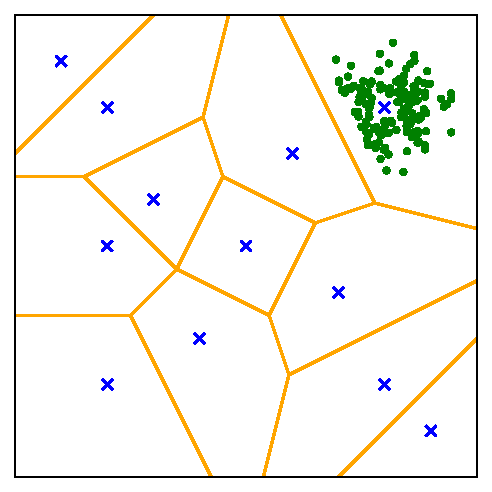
\includegraphics[width=0.24\textwidth]{figs/voronoi_partition/scenario1.pdf}
        }
	\subfloat[]{         
        \label{fig:voronoi partition b}  
		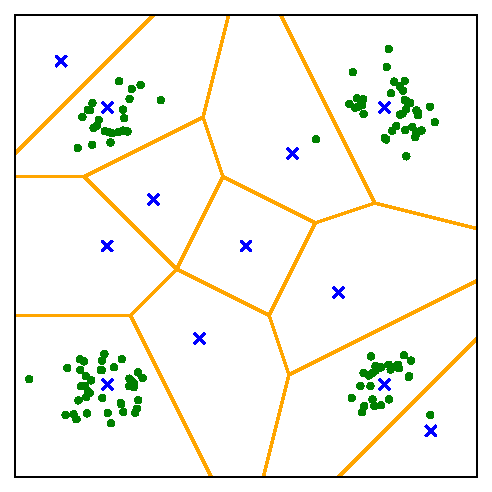
\includegraphics[width=0.24\textwidth]{figs/voronoi_partition/scenario2.pdf}
        }
	\subfloat[]{         
        \label{fig:voronoi partition c}  
		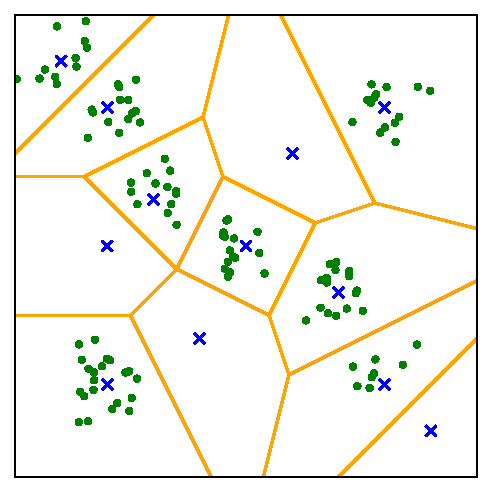
\includegraphics[width=0.24\textwidth]{figs/voronoi_partition/scenario3.pdf}
        }
    \subfloat[]{         
        \label{fig:voronoi partition d}  
		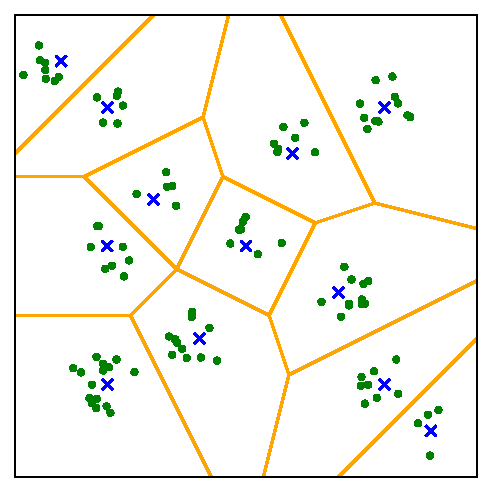
\includegraphics[width=0.24\textwidth]{figs/voronoi_partition/scenario4.pdf}
        }
    \vspace{-1ex}
	\caption{Visualization of the Voronoi partition. The symbols $\cdot$ and $\times$ represent the feature and code vectors, respectively.}
    \vspace{-3ex}
	\label{fig:visualization of voronoi partition}
\end{figure*}

\subsection{Voronoi Partition: Definition and Connection to Codebook Collapse}
\label{appendix:voronoi partition definition}

Let $\mathcal{X}$ be a metric space with distance function $d(\cdot, \cdot)$, and let $\{\be_k\}_{k=1}^K$ denote a set of code vectors. The Voronoi cell (or Voronoi region) $\mathcal{R}_k$ associated with code vector $\be_k$ is the set of all points in $\mathcal{X}$ whose distance to $\be_k$ is no greater than their distance to any other code vector $\be_j$ ($j \neq k$):
\begin{align}
\mathcal{R}_k = \{x \in \mathcal{X} \;|\; d(x, \be_k) \le d(x, \be_j), \forall j \neq k\}.
\end{align}
The Voronoi diagram is the collection of all cells $\{\mathcal{R}_k\}_{k=1}^K$. Figure~\ref{fig:visualization of voronoi partition} illustrates a Voronoi diagram for 12 code vectors, partitioning the metric space into 12 regions according to $\mathcal{R}_k$. When $d$ is the $\ell_2$ distance, vector quantization (VQ) can equivalently be expressed in terms of Voronoi regions:
\begin{align}
\label{eq:vq voronoi partition}
\forall \bz_i \in \mathcal{R}_j, \quad \bz_i' = \argmin_{\be \in \{\be_k\}} \norm{\bz_i - \be} = \be_j,
\end{align}
where $\bz_i$ is an arbitrary feature vector. Equation~\ref{eq:vq voronoi partition} provides an alternative viewpoint for nearest neighbor search: identify the region $\mathcal{R}_j$ containing $\bz_i$ and select the corresponding code vector $\be_j$.

\paragraph{Relation to Codebook Collapse} 
Codebook collapse occurs in its most severe form when all feature vectors fall within the same Voronoi region. As illustrated in Figure~\ref{fig:voronoi partition a}, all features occupy a single region, leading to the utilization of only one code vector. To prevent collapse, feature vectors should be distributed across all regions as uniformly as possible (Figure~\ref{fig:voronoi partition d}).

\subsection{Limitations of Existing Vector Quantization Methods}
\label{appendix:VQ codebook collapse}

We analyze why standard VQ methods often fail to prevent codebook collapse, using Vanilla VQ~\cite{Oord2017NeuralDR} and $k$-means-based VQ~\cite{Razavi2019GeneratingDH} as examples. Both share a similar assignment step but differ in their update mechanisms. 

\paragraph{Assignment Step} 
Given feature vectors $\{\bz_i\}_{i=1}^N$ and code vectors $\{\be_k\}_{k=1}^K$, at iteration $t$, both methods partition the feature space into Voronoi cells and assign features to the nearest code vectors:
\begin{align}
\mathcal{R}_k^{(t-1)} = \{x \in \mathcal{X} \;|\; \left\Vert x- \be_k^{(t-1)} \right\Vert_2^{2} \le \left\Vert x- \be_j^{(t-1)} \right\Vert_2^{2}, \forall j \neq k\}, \quad \mathcal{S}_{k}^{(t)} = \{\bz_i \;|\; \bz_i \in \mathcal{R}_k^{(t-1)}\}. \nonumber
\end{align}

\paragraph{Update Step in Vanilla VQ} Code vectors are updated via gradient descent on the reconstruction loss:
\begin{align}
\mathcal{L} = \frac{1}{N}\sum_{k=1}^{K}\sum_{\bz_m \in \mathcal{S}_{k}^{(t)}} \left\Vert \bz_m - \be_k^{(t-1)} \right\Vert_2^{2}.
\end{align}

\paragraph{Update Step in $k$-means-based VQ} Code vectors are updated using an exponential moving average:
\begin{align}
\be_k^{(t)} = \alpha \be_k^{(t-1)} + (1-\alpha) \frac{1}{|\mathcal{S}_{k}^{(t)}|} \sum_{\bz_m \in \mathcal{S}_{k}^{(t)}} \bz_m.
\end{align}

\paragraph{Codebook Collapse in Vanilla and $k$-means VQ} 
Despite different update strategies, both methods can suffer from codebook collapse because the assignment step does not guarantee that all Voronoi cells receive feature vectors (Figures~\ref{fig:voronoi partition a}--\ref{fig:voronoi partition c}). Larger codebooks exacerbate the issue, leaving some cells unassigned and their corresponding code vectors underutilized.

\paragraph{Connection to Distribution Matching and Mitigation} 
As demonstrated in Section~\ref{sec:atomic setting}, both VQ methods are sensitive to codebook initialization. Collapse is mitigated only if the codebook distribution approximates the feature distribution. However, in practice, feature distributions are typically unknown and dynamically evolving. To address this, we introduce a \textbf{distributional matching constraint} that aligns the codebook distribution with the feature distribution, ensuring complete codebook utilization.


\iffalse
\subsection{The Definition of Voronoi Partition and The Connection to Codebook Collapse}
\label{appendix:voronoi partition definition}
Let $\mathcal{X}$ be a metric space with distance function $d(\cdot, \cdot)$, and given a set of code vectors $\{\be_k\}_{k=1}^K$. The Voronoi cell, or Voronoi region, $\mathcal{R}_k$, associated with the code vector $\be_k$ is the set of all points in 
$\mathcal{X}$ whose distance to $\be_k$ is not greater than their distance to the other code vectors $\be_j$, where $j$ is any index different from $k$. Mathematically, this can be expressed as:
\begin{align}
\mathcal{R}_k = \{x \in \mathcal{X}; d(x, \be_k) \leq d(x, \be_j), \forall j \neq k\},
\end{align}
The Voronoi diagram is simply the tuple of cells $\{\mathcal{R}_k\}_{k=1}^K$. As depicted in Figure~\ref{fig:visualization of voronoi partition}, there are 12 code vectors which partition the metric space into 12 regions according to the $\mathcal{R}_k$. When $d$ is a a distance function based on the $\ell_2$ norm, the vector quantization (VQ) process can be equivalently understood through the regions $\mathcal{R}_k$ as:
\begin{align}
\label{eq:vq voronoi partition}
\forall \bz_i \in \mathcal{R}_j, \quad \bz_i' = \argmin_{\be\in\{\be_k\}}\norm{\bz_i-\be} = \be_j
\end{align}
Where $\bz_i$ is an arbitrary feature vector.  Equation~\ref{eq:vq voronoi partition} offers an alternative approach for nearest neighbor search in code vector selection. Specifically, this involves first identifying the partition region $\mathcal{R}_j$ to which the feature vector $\bz_i$ belongs, and then directly obtaining the nearest code vector $\be_j$ based on the region’s id $j$.

\paragraph{Relation to Codebook Collapse} 
The most severe case of codebook collapse occurs when all feature vectors belong to the same partition region. As illustrated in Figure~\ref{fig:voronoi partition a}, all feature vectors are confined to a single partition region in the upper right corner, resulting in the utilization of only one code vector. To prevent codebook collapse, it is crucial for feature vectors to be distributed across all partition regions as evenly as possible, as depicted in Figure~\ref{fig:voronoi partition d}.


\subsection{Why Existing Vector Quantization Strategies Fail to Address Codebook Collapse}
\label{appendix:VQ codebook collapse}

This section offers an in-depth analysis of why existing VQ methods inherently struggle to address codebook collapse. We use Vanilla VQ~\cite{Oord2017NeuralDR} and VQ methods based on the $k$-means algorithm~\cite{Razavi2019GeneratingDH} as illustrative examples. These two approaches share similarities in their assignment step but differ in their update mechanisms. 

\paragraph{Assignment Step} 
Suppose there is a set of feature vectors $\{\bz_i\}_{i=1}^N$ and code vectors $\{\be_k\}_{k=1}^K$. In the $t$-th assignment step, both algorithms partition the feature space into Voronoi cells, based on which we assign all feature vectors to their nearest code vectors as follows: 
\begin{align}
\mathcal{R}_k^{(t-1)} = \{x \in \mathcal{X}; \left\Vert x- \be_k^{(t-1)} \right\Vert_2^{2} \leq \left\Vert x- \be_j^{(t-1)} \right\Vert_2^{2}, \forall j \neq k\}, \quad \mathcal{S}_{k}^{(t)} = \{\bz_i; \bz_i \in \mathcal{R}_k^{(t-1)}\}
\vspace{-10pt}
\end{align}

\paragraph{Update Step in Vanilla VQ} It updates the code vectors using gradient descent through the loss function provided below.
\begin{align}
\mathcal{L} = \frac{1}{N}\sum_{k=1}^{K}\sum_{z_m \in \mathcal{S}_{k}^{(t)}} \left\Vert \bz_m - \be_k^{(t-1)} \right\Vert_2^{2} 
\vspace{-10pt}
\end{align} 
 
\paragraph{Update Step in $k$-means-based VQ} It updates the code vectors by using an exponential moving average of the feature vectors assigned to each code vector:
\begin{align}
\be_k^{(t)} = \alpha \be_k^{(t-1)} + (1-\alpha) \frac{1}{|\mathcal{S}_{k}^{(t)}|} \sum_{\bz_m \in \mathcal{S}_{k}^{(t)}} \bz_m
\vspace{-10pt}
\end{align} 

\paragraph{Codebook Collapse in Two VQs} While both VQ methods employ different update strategies for the code vectors, they still suffer from codebook collapse. This is because, in the assignment step, the learnable Voronoi partition does not guarantee that all Voronoi cells will be assigned feature vectors, as illustrated in Figures~\ref{fig:voronoi partition a} to~\ref{fig:voronoi partition c}. Especially when the codebook size is large, there are more Voronoi cells, and inevitably, some cells remain unassigned. In such cases, the corresponding code vectors remain unupdated and underutilized.

\paragraph{Connection to Distribution Matching and Solutions} In Section~\ref{sec:atomic setting}, we demonstrated through synthetic experiments that the effectiveness of both VQ methods heavily relies on the codebook initialization. Only when the codebook distribution is initialized to approximate the feature distribution can codebook collapse be effectively mitigated. However, in practical applications, the feature distribution is often unknown and evolves dynamically during training. To address this issue, we propose an explicit distributional matching constraint that ensures the codebook distribution aligns closely with the feature distribution, thereby achieving 100\% codebook utilization.
\fi

\section{The Relationship Between Gradient Gap and Quantization Error}
\label{appendix:gradient gap quantization error}

In this section, we provide a formal derivation of the relationship between the \textbf{Quantization Error} (Criterion 1) and the \textbf{Gradient Gap} caused by the Straight-Through Estimator (STE). This analysis theoretically supports our claim that minimizing quantization error via distribution matching inherently mitigates training instability.

\textbf{Problem Setup}: Let $\mathcal{L}$ denote the global loss function. In the VQ process, the encoder outputs a continuous latent vector $z_e$, which is discretized to a code $z_q$. 
During backpropagation, the non-differentiable quantization operation is bypassed using the STE, which approximates the gradient of the encoder output $\frac{\partial \mathcal{L}}{\partial z_e}$ using the gradient of the quantized code $\frac{\partial \mathcal{L}}{\partial z_q}$:
\begin{equation}
    \text{STE Approximation:} \quad \frac{\partial \mathcal{L}}{\partial z_e} \leftarrow \frac{\partial \mathcal{L}}{\partial z_q}
\vspace{-3pt}
\end{equation}
We define the \textbf{Gradient Gap} ($\mathcal{G}$) as the magnitude of the discrepancy between the true gradient and the STE approximated gradient:
\begin{equation}
    \mathcal{G} \triangleq \left\| \frac{\partial \mathcal{L}}{\partial z_e} - \frac{\partial \mathcal{L}}{\partial z_q} \right\|
\vspace{-3pt}
\end{equation}

\textbf{Taylor Expansion Analysis}: To analyze this gap, we perform a Taylor expansion of the gradient function around the quantized point $z_q$. Let us consider the gradient function with respect to the latent variable $x$. Expanding $\frac{\partial \mathcal{L}}{\partial z_e}$ at the point $x = z_q$, we obtain:

\begin{equation}
    \frac{\partial \mathcal{L}}{\partial z_e} = \left. \frac{\partial \mathcal{L}}{\partial x} \right|_{x=z_q} + \left. \frac{\partial^2 \mathcal{L}}{\partial x^2} \right|_{x=z_q} (z_e - z_q) + \mathcal{O}(\|z_e - z_q\|^2)
    \label{eq:taylor}
\vspace{-3pt}
\end{equation}

where $\left. \frac{\partial \mathcal{L}}{\partial x} \right|_{x=z_q}$ is exactly the gradient backpropagated from the quantized code, i.e., $\frac{\partial \mathcal{L}}{\partial z_q}$, and $\mathbf{H} = \left. \frac{\partial^2 \mathcal{L}}{\partial x^2} \right|_{x=z_q}$ is the Hessian matrix, representing the local curvature of the loss function at $z_q$.

\textbf{First-Order Approximation and Upper Bound}: By retaining only the first-order term (as is common in gradient gap analysis) and ignoring the higher-order terms $\mathcal{O}(\|z_e - z_q\|^2)$, the relationship can be approximated as:

\begin{equation}
    \frac{\partial \mathcal{L}}{\partial z_e} \approx \frac{\partial \mathcal{L}}{\partial z_q} + \mathbf{H} (z_e - z_q)
\vspace{-3pt}
\end{equation}

Substituting this back into the definition of the Gradient Gap $\mathcal{G}$, we get:
\begin{equation}
    \mathcal{G} = \left\| \frac{\partial \mathcal{L}}{\partial z_e} - \frac{\partial \mathcal{L}}{\partial z_q} \right\| \approx \| \mathbf{H} (z_e - z_q) \|
\vspace{-3pt}
\end{equation}

By applying the definition of the consistent matrix norm (specifically, the spectral norm for the symmetric Hessian), we derive the upper bound:

\begin{equation}
    \mathcal{G} \le \| \mathbf{H} \|_2 \cdot \| z_e - z_q \|
    \label{eq:bound}
\vspace{-3pt}
\end{equation}
where $\| \mathbf{H} \|_2$ represents the spectral norm of the Hessian (indicative of the maximum curvature) and $\| z_e - z_q \|$ corresponds to the \textbf{Quantization Error}.


The derivation in Eq. \ref{eq:bound} explicitly demonstrates that the Gradient Gap $\mathcal{G}$ is linearly bounded by the Quantization Error. In methods like Vanilla VQ, a large Quantization Error implies a looser bound on $\mathcal{G}$, leading to inaccurate gradient signals passed to the encoder. This large discrepancy causes the ``Training Instability'' observed in previous works. By minimizing the Wasserstein distance, our method explicitly minimizes the Quantization Error (Criterion 1). This tightens the upper bound on $\mathcal{G}$, ensuring that the gradient passed to the encoder ($\frac{\partial \mathcal{L}}{\partial z_q}$) is a faithful approximation of the true gradient ($\frac{\partial \mathcal{L}}{\partial z_e}$).

\section{Complementary Roles of Criterion~\ref{criteria:cu} and~\ref{criteria:cp} in Assessing Codebook Collapse} 
\label{appendix:explanation on criterions}

\begin{figure*}[!h]
    \vspace{-6ex}
	\centering
	\subfloat[$(50\%, 4.92)$]{         
        \label{fig:criterion sample a}  
         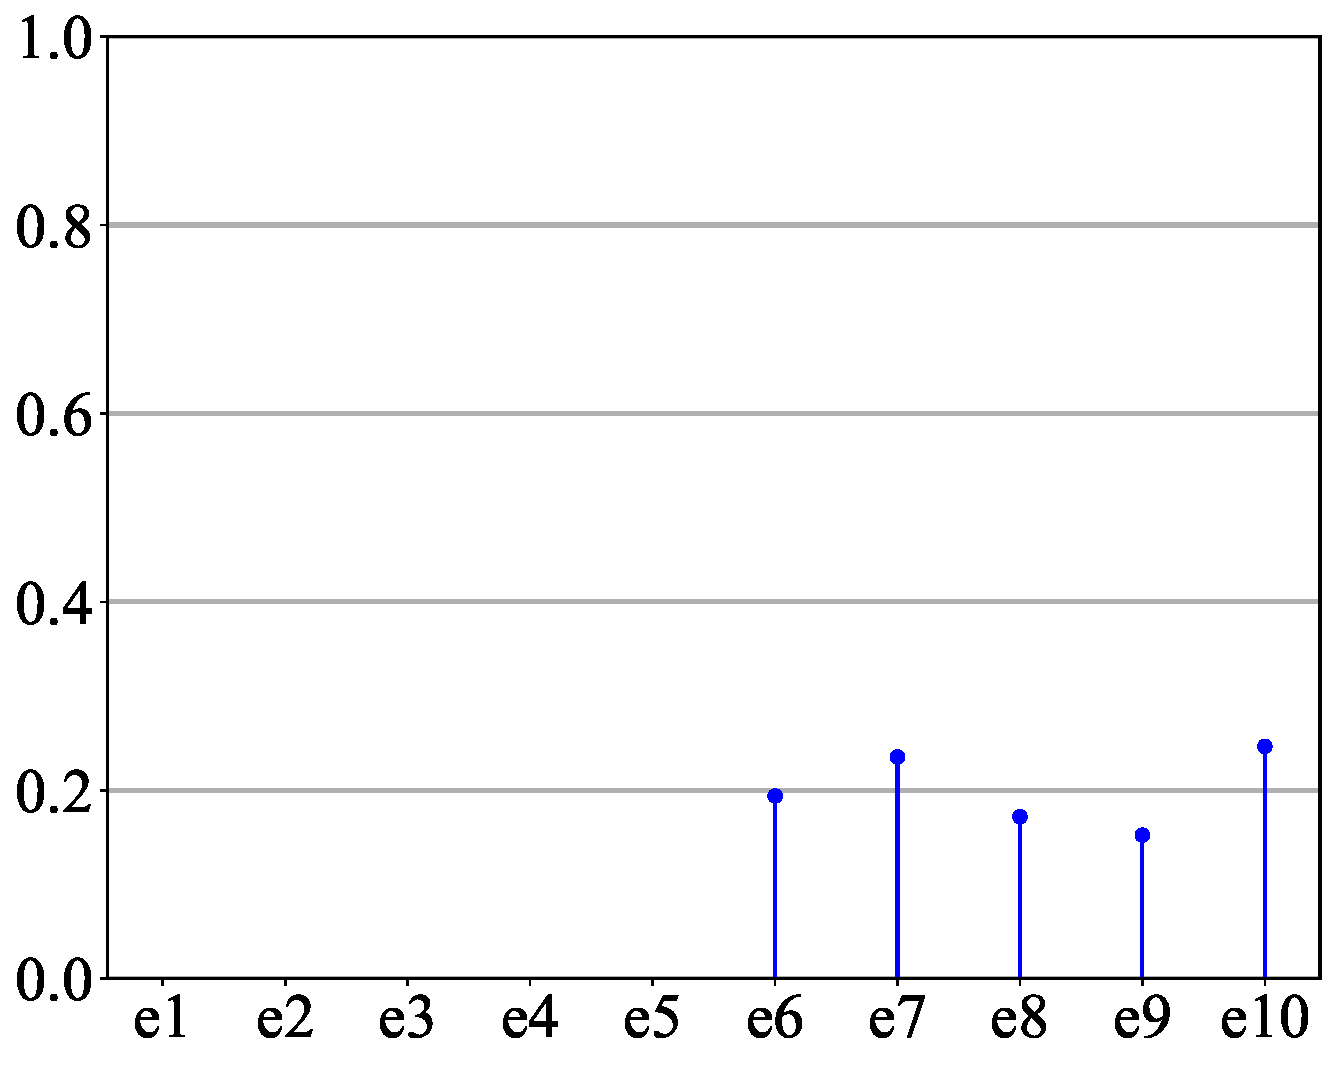
\includegraphics[width=0.23\textwidth]{figs/criterion_examples/a.pdf}
        }
	\subfloat[$(100\%, 10.00)$]{        
        \label{fig:criterion sample b}  
		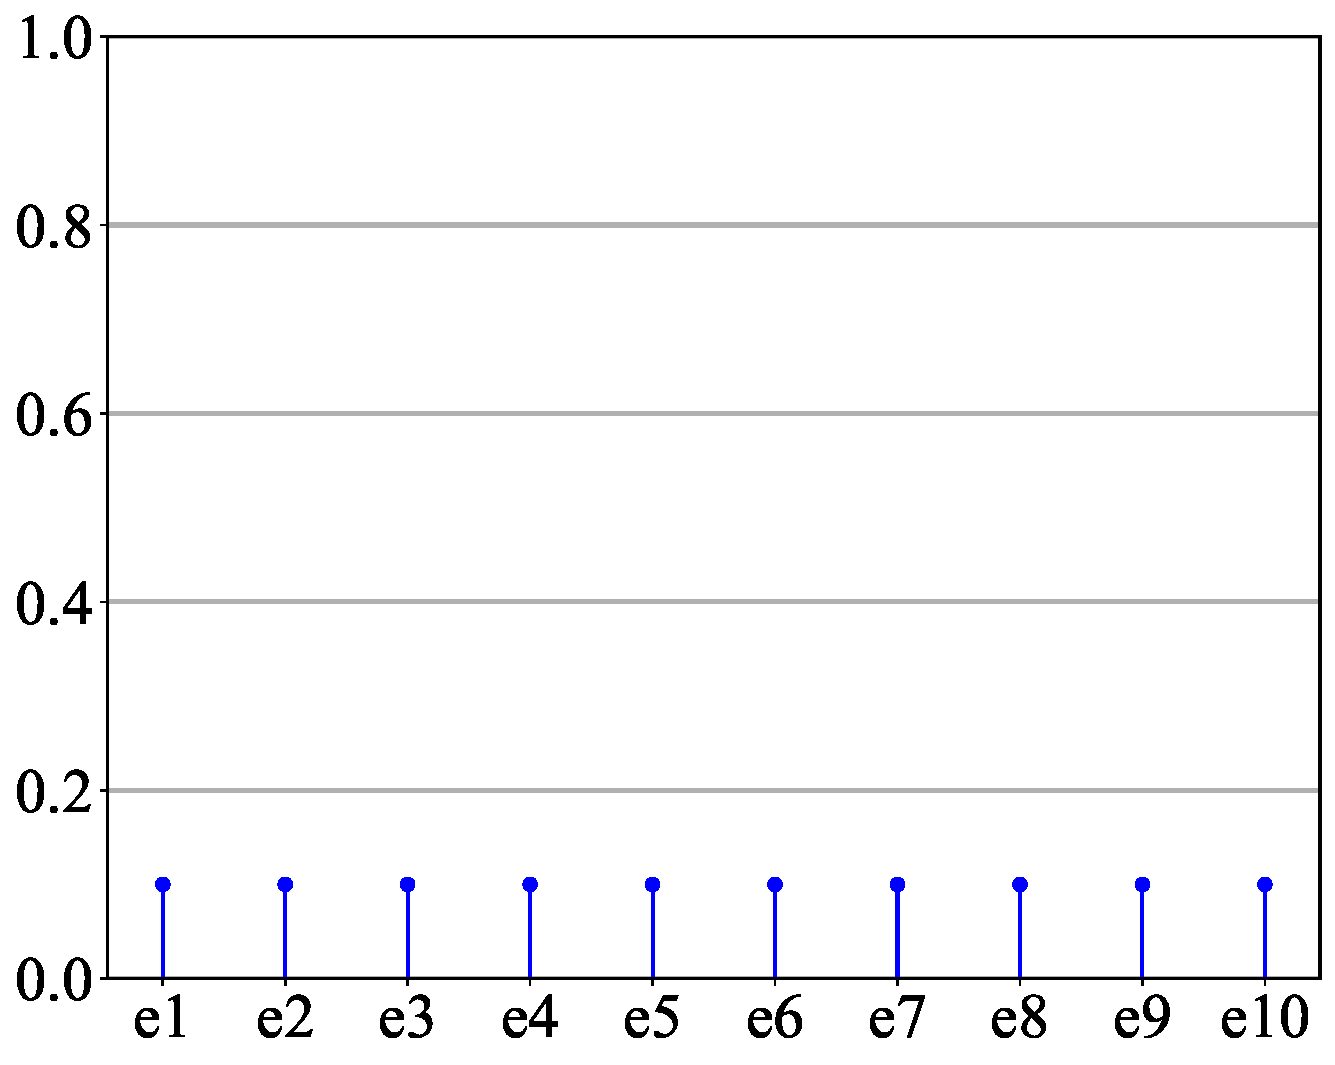
\includegraphics[width=0.23\textwidth]{figs/criterion_examples/b.pdf}
        }
	\subfloat[$(100\%, 1.02)$]{         
        \label{fig:criterion sample c}  
		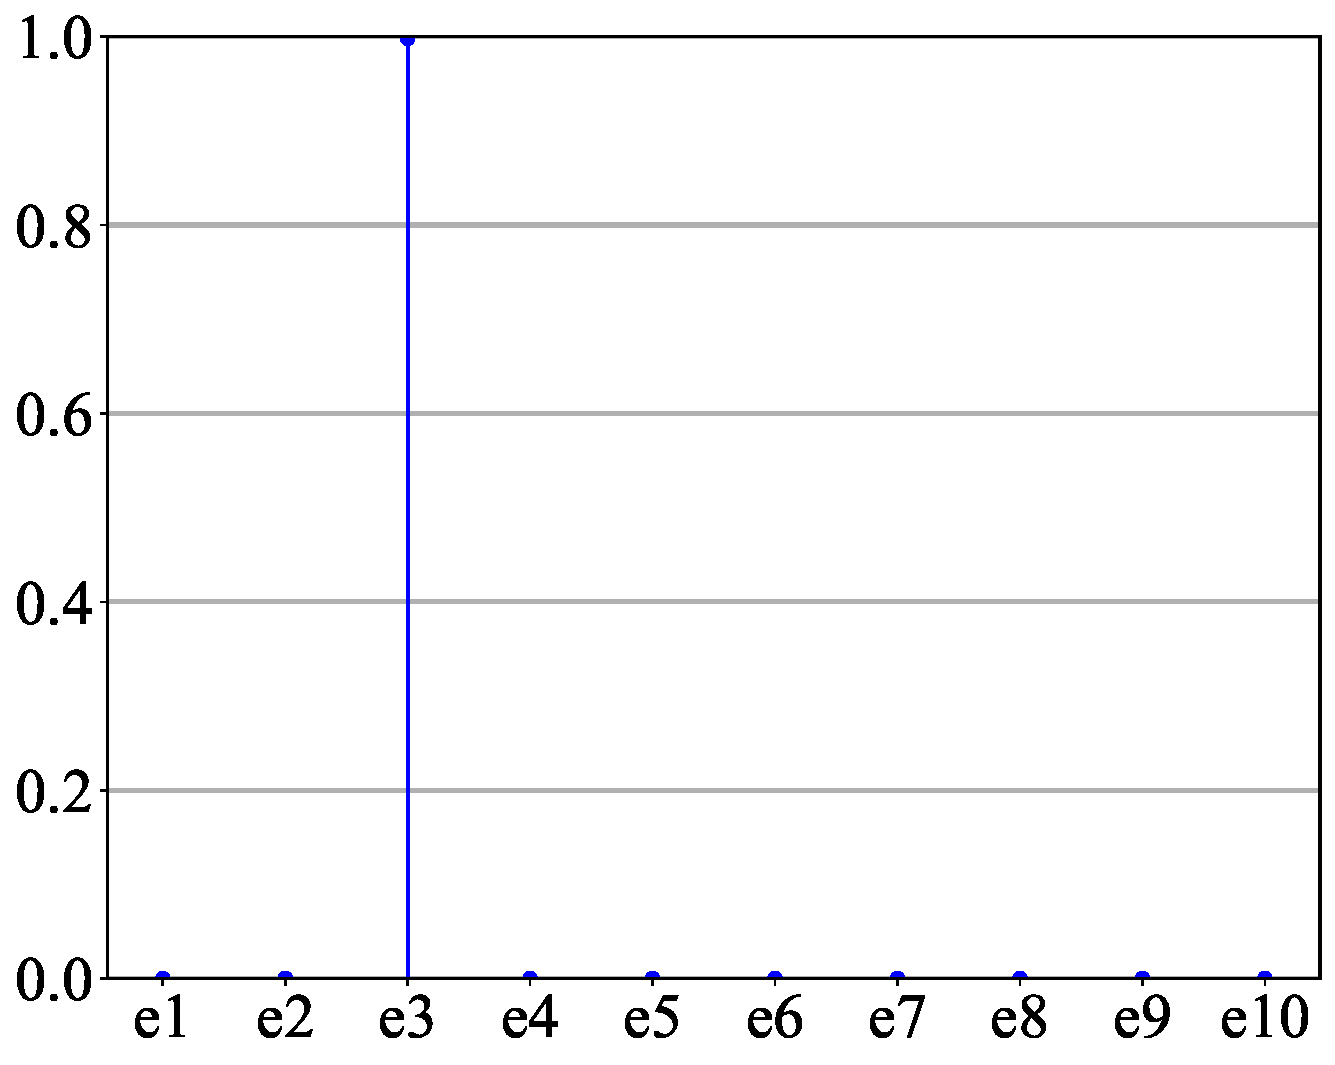
\includegraphics[width=0.23\textwidth]{figs/criterion_examples/c.pdf}
        }
    \subfloat[$(100\%, 4.92)$]{         
        \label{fig:criterion sample d}  
		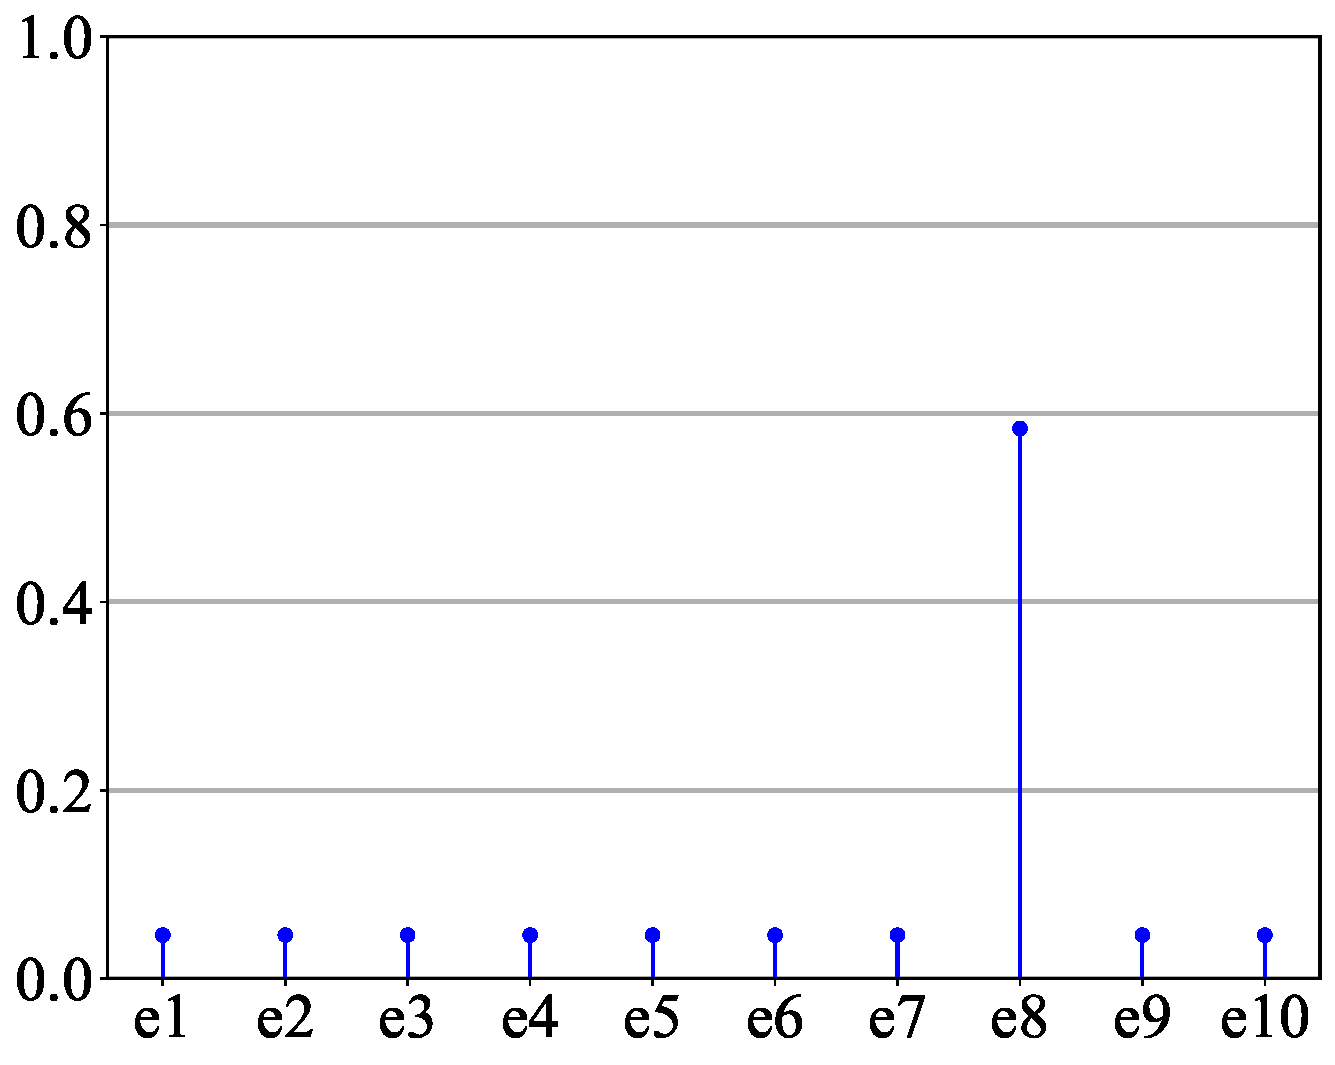
\includegraphics[width=0.23\textwidth]{figs/criterion_examples/d.pdf}
        }
    \vspace{-1ex}
	\caption{Visualization of the evaluation criteria $(\cU, \cC)$.}
    \vspace{-2ex}
	\label{fig:visualization of criterion triple}
\end{figure*}

To clarify the complementary roles of Criterion~\ref{criteria:cu} and Criterion~\ref{criteria:cp}, which are introduced in Section~\ref{sec:distributional formulation}, we provide visual illustrations to facilitate intuitive understanding. The metric $\mathcal{U}$ is designed to quantify the \emph{completeness} of codebook utilization. As shown in Figures~\ref{fig:criterion sample a} and~\ref{fig:criterion sample b}, the corresponding values of $\mathcal{U}$ are $50\%$ and $100\%$, respectively\footnote{This difference arises because, in Figure~\ref{fig:criterion sample a}, only half of the code vectors have nonzero utilization probabilities $p_k$, as defined in Criterion~\ref{criteria:cp}, whereas in Figure~\ref{fig:criterion sample b}, all code vectors satisfy $p_k>0$.}.

However, $\mathcal{U}$ alone is insufficient to characterize the severity of codebook collapse, since it does not account for imbalance among utilized code vectors. This limitation is illustrated in Figure~\ref{fig:criterion sample c}. Although all code vectors are utilized, resulting in $\mathcal{U}=100\%$, the code vector $e_3$ overwhelmingly dominates the assignment distribution. Such extreme imbalance constitutes a degenerate form of codebook collapse, even though $\mathcal{U}$ attains its maximum value. This observation motivates the introduction of Criterion~\ref{criteria:cp}, which explicitly measures the uniformity, or conversely the imbalance, of codebook utilization.

A comparison between Figures~\ref{fig:criterion sample b} and~\ref{fig:criterion sample c} further highlights the discriminative capability of Criterion~\ref{criteria:cp}. While both cases share the same utilization completeness, namely $\mathcal{U}=100\%$, their corresponding values of $\mathcal{C}$ differ substantially, being $10.00$ and $1.02$, respectively. This contrast demonstrates that Criterion~\ref{criteria:cp} effectively captures differences in the distribution of $p_k$ that are not reflected by $\mathcal{U}$. In particular, the near minimal value of $\mathcal{C}$ in Figure~\ref{fig:criterion sample c} correctly identifies this scenario as a collapsed codebook, which aligns with our intended interpretation.

Nevertheless, Criterion~\ref{criteria:cp} alone is also insufficient for a comprehensive evaluation of codebook collapse. As illustrated by Figures~\ref{fig:criterion sample a} and~\ref{fig:criterion sample d}, identical values of $\mathcal{C}$ can correspond to markedly different levels of utilization completeness, as indicated by their substantially different values of $\mathcal{U}$. This discrepancy shows that $\mathcal{C}$ by itself cannot quantify the proportion of actively utilized code vectors.

Consequently, in this work, we adopt the joint use of Criterion~\ref{criteria:cu} and Criterion~\ref{criteria:cp} to quantitatively assess codebook collapse. Effective mitigation is achieved only when both metrics attain sufficiently large values, indicating that the codebook is both fully utilized and balanced in its assignment distribution.

\section{The Significant Impact of Distribution Variance on Quantization Error} 
\label{appendix:Impact of Distribution Variance}
As discussed in Section~\ref{sec:effects of distribution matching} and~\ref{sec:theoretical analysis}, the optimal criterion triple is achieved when the distributions $\mathcal{P}_A$ and $\mathcal{P}_B$ are identical. In this section, we further analyze the criterion triple by the lens of distribution variance under the condition that both distributions are identical. Specifically, we first sample a set of feature vectors $\{\bz_i\}_{i=1}^N$ along with a set of code vectors $\{\be_k\}_{k=1}^K$ from the distribution $\mathcal{N}_d(\m 0, \sigma^2\bm I)$ or the distribution $\unif_d(-\zeta, \zeta)$. We then calculate the evaluation criteria according to their definitions in Section~\ref{sec:distributional formulation}. As demonstrated in Table~\ref{table:distribution variance}, $\sigma$ and $\zeta$ have a substantial impact on $\cE$, while $\cU$ and $\mathcal{C}$ remains largely unaffected. 

\begin{table*}[!h]  
\centering
\vspace{-2ex}
\caption{The criterion triple influence by the distribution variance.}
\vspace{-1ex}
\resizebox{0.9\textwidth}{!}{
\begin{tabular}{c|c|c|c|c|c|c|c|c|c|c|}\hline
\multirow{2}{*}{Evaluation Criteria}  & \multicolumn{5}{|c}{$\sigma$} & \multicolumn{5}{|c}{$\zeta$}\\\cline{2-11} 
& 0.0001 & 0.001 & 0.01 & 0.1 & 1.0 & 0.0001 & 0.001 & 0.01 & 0.1 & 1.0 \\\hline
$\cE$  & 1.25e-8 & 1.25e-6 & 1.25e-4 & 1.24e-2 & 1.25 & 3.27e-9 & 3.27e-7 & 3.27e-5 & 3.27e-3 & 0.327 \\
$\cU$ & 0.9934 & 0.9938 & 0.9940 & 0.9934 & 0.9941 & 0.9993 & 0.9986 & 0.9990 & 0.9992 & 0.9989 \\
$\mathcal{C}$ & 7265.3 & 7260.3 & 7267.7 & 7255.0  & 7275.8 & 7380.2 & 7372.2 & 7387.9 & 7397.5 & 7391.6 \\\hline
\end{tabular}}
\vspace{-2ex}
\label{table:distribution variance}
\end{table*}

This experimental finding suggests that when the distribution variance of the feature vectors is uncontrollable or unknown, reporting a comparison of quantization error among various VQ methods is unreasonable. This is because the improvement in quantization error is predominantly attributed to the reduction in distribution variance rather than the effectiveness of the VQ methods. To evaluate various VQ methods in terms of the criterion triple, we establish an atomic and fair experimental setting in Section~\ref{sec:atomic setting}, where the feature distributions for all VQ methods are identical.

\section{Interpretation of Qualitative Distributional Matching Results}
\label{appendix:prototypical study}

This section interprets the experimental results presented in Figure~\ref{fig:criterion triple analysis}. The VQ process relies on nearest neighbor search for code vector selection. As evident from Figure~\ref{fig:diagram 1 group 1} to~\ref{fig:diagram 4 group 1}, actively selected code vectors are predominantly those located in close proximity to or within the feature distribution, while distant ones remain unselected. This leads to highly uneven code vector utilization $p_k$, with those closer to the feature distribution being excessively used. This elucidates the significantly low $\mathcal{U}$ and $\mathcal{C}$ observed in Figure~\ref{fig:diagram 1 group 1}. Furthermore, a notable quantization error, e.g., $\mathcal{E}=1.19$ in Figure~\ref{fig:diagram 1 group 1}, arises when the codebook and feature distributions are mismatched, forcing feature vectors outside the codebook to settle for distant code vectors. Conversely, as the disk centers align, leading to a closer match between the two distributions, an increased number of code vectors become actively engaged. Additionally, code vectors are utilized more uniformly, and feature vectors can select nearer counterparts. This accounts for the improvement of criterion triple values towards optimality as the distributions align.

Analogously, we can employ nearest neighbor search to interpret the second case. When code vectors are distributed within the range of feature vectors, as illustrated in Figure~\ref{fig:diagram 1 group 2} and Figure~\ref{fig:diagram 2 group 2}, the majority of code vectors would be actively utilized, ensuring high $\mathcal{U}$. However, the utilization of these code vectors is not uniform; code vectors on the periphery of the codebook distribution are more frequently used, leading to relatively low $\mathcal{C}$. Feature vectors on the periphery will have larger distances to their nearest code vectors, resulting in higher $\mathcal{E}$. Conversely, when feature vectors fall within the range of code vectors, as depicted in Figure~\ref{fig:diagram 3 group 2} and Figure~\ref{fig:diagram 4 group 2}, outer code vectors remain largely unused, leading to a lower $\mathcal{U}$ and $\mathcal{C}$. Since only inner code vectors are active, each feature vector can find a nearby counterpart, maintaining low $\mathcal{E}$.

\section{Supplementary Quantitative Analyses on Distribution Matching: Further Supporting the Main Findings in Section~\ref{sec:effects of distribution matching}}
\label{appendix:supplementary comprehensive quantitative analyses}
To further elucidate the effects of the distributional matching, we conduct more quantitative analyses centered around the criterion triple $(\cE, \cU, \mathcal{C})$.

\subsection{Codebook Distribution and Feature Distribution are Gaussian Distributions}
\label{appendix:analyses under gaussian distribution}

\begin{figure*}[!t]
    \vspace{-2ex}
    \centering

    
    %%%%%%%%%%%%%%%%%%%%% Row 1: Quantization Error %%%%%%%%%%%%%%%%%%%%%
    \subfloat[$\cE$ {w.r.t.} $K$]{ 
        \label{fig:gaussian_codebooksize_mean_error}  
        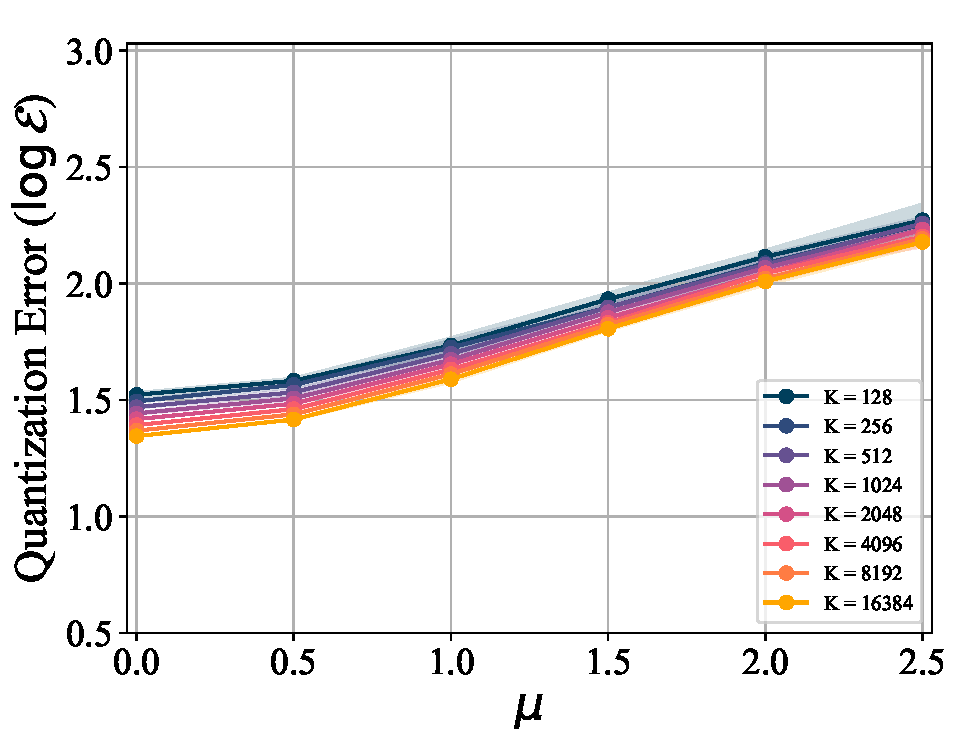
\includegraphics[width=0.16\textwidth]{figs/quantitative_analyses/gaussian_distribution/CodebookSize_mean_Quant.pdf}
    }
    \hspace{-0.39cm}
    \subfloat[$\cE$ {w.r.t.} $d$]{
        \label{fig:gaussian_featuredim_mean_error}
        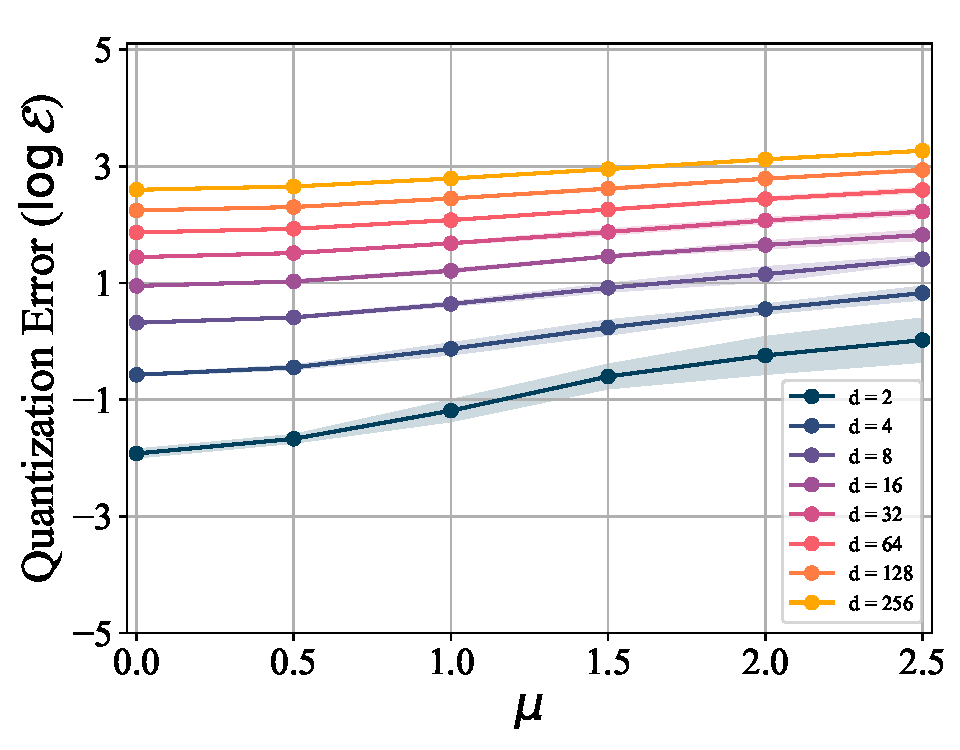
\includegraphics[width=0.16\textwidth]{figs/quantitative_analyses/gaussian_distribution/FeatureDim_mean_Quant.pdf}
    }
    \hspace{-0.39cm}
    \subfloat[$\cE$ {w.r.t.} $N$]{
        \label{fig:gaussian_featuresize_mean_error}
        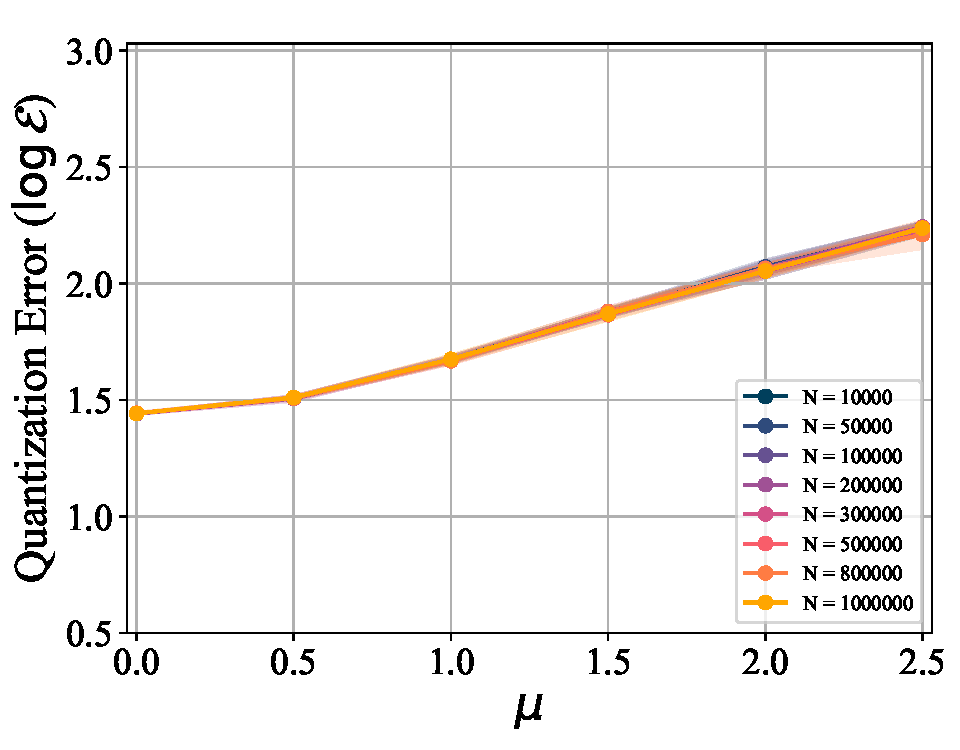
\includegraphics[width=0.16\textwidth]{figs/quantitative_analyses/gaussian_distribution/FeatureSize_mean_Quant.pdf}
    }
    \hspace{-0.39cm}
    \subfloat[$\cE$ {w.r.t.} $K$]{ 
        \label{fig:gaussian_codebooksize_sigma_error}  
        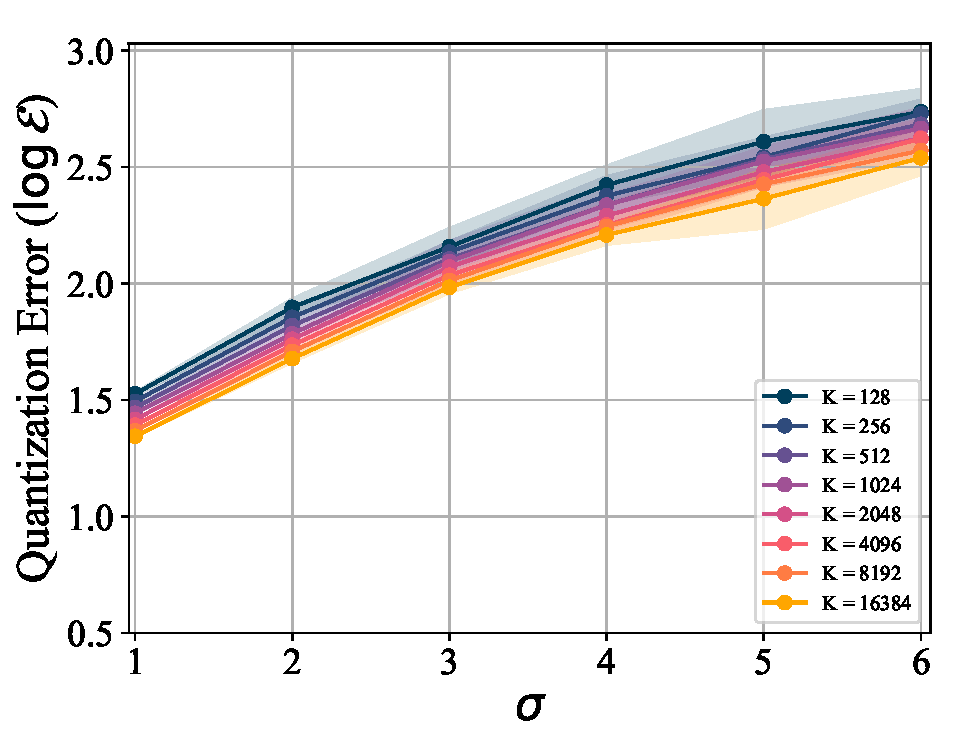
\includegraphics[width=0.16\textwidth]{figs/quantitative_analyses/gaussian_distribution/CodebookSize_Var_Quant.pdf}
    }
    \hspace{-0.39cm}
    \subfloat[$\cE$ {w.r.t.} $d$]{
        \label{fig:gaussian_featuredim_sigma_error}
        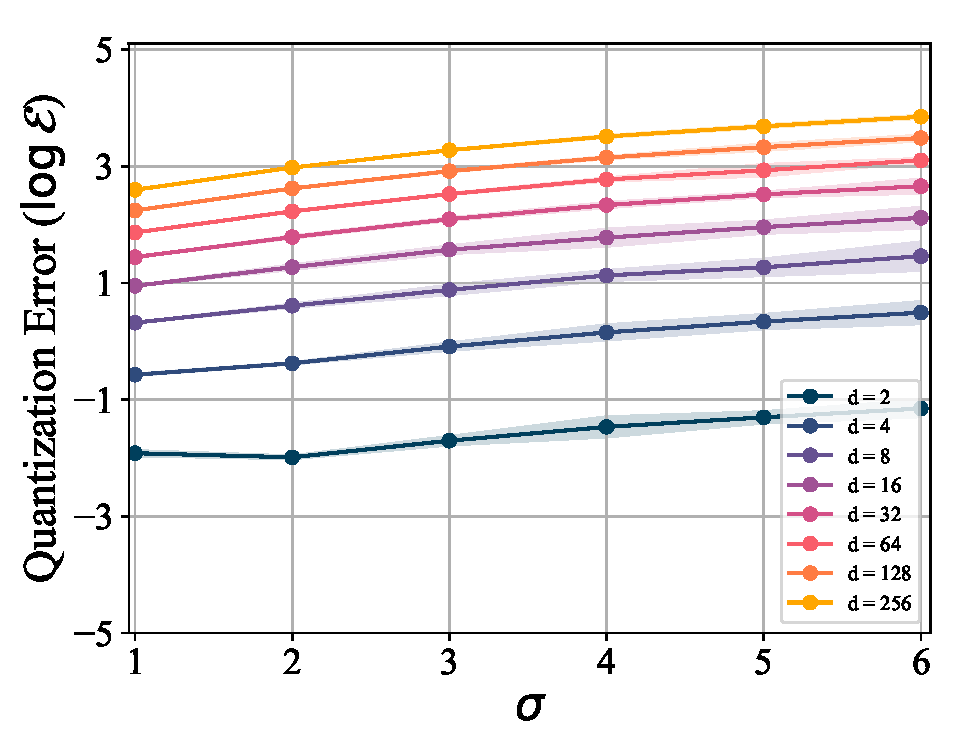
\includegraphics[width=0.16\textwidth]{figs/quantitative_analyses/gaussian_distribution/FeatureDim_Var_Quant.pdf}
    }
    \hspace{-0.39cm}
    \subfloat[$\cE$ {w.r.t.} $N$]{
        \label{fig:gaussian_featuresize_sigma_error}
        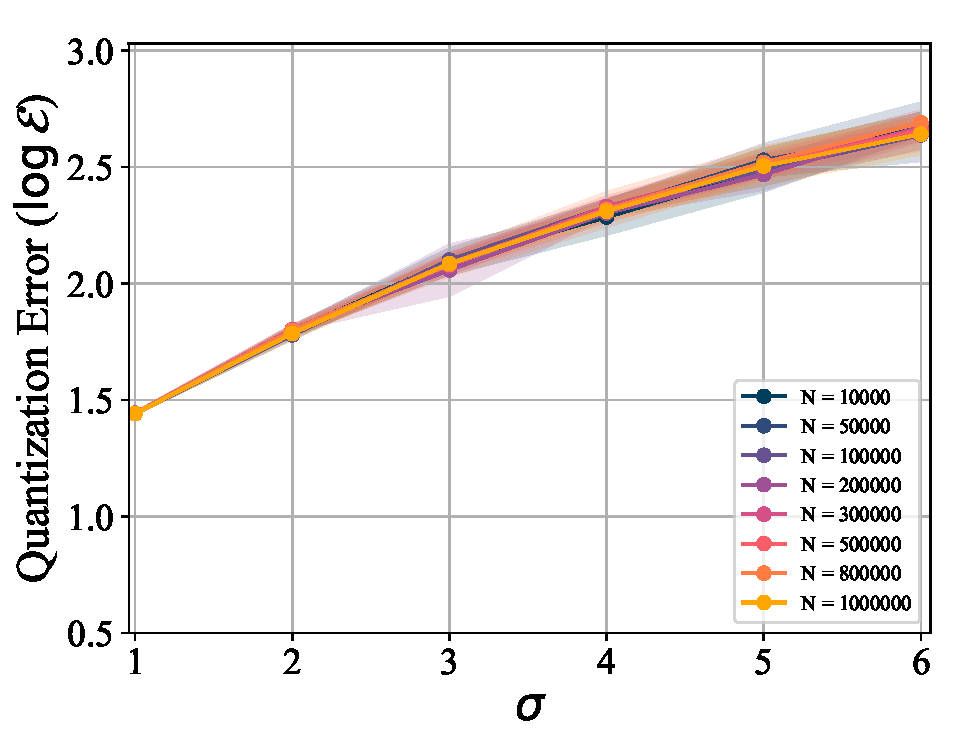
\includegraphics[width=0.16\textwidth]{figs/quantitative_analyses/gaussian_distribution/FeatureSize_Var_Quant.pdf}
    }

    %%%%%%%%%%%%%%%%%%%%% Row 2: Codebook Utilization %%%%%%%%%%%%%%%%%%%%%
    \subfloat[$\cU$ {w.r.t.} $K$]{ 
        \label{fig:gaussian_codebooksize_mean_utilization}  
        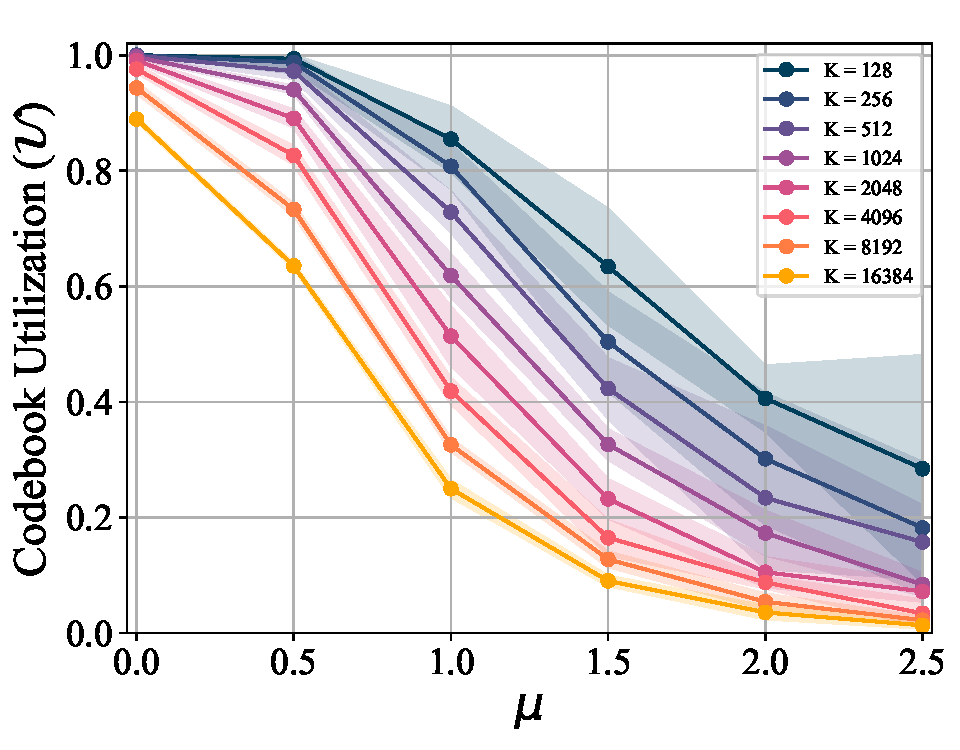
\includegraphics[width=0.16\textwidth]{figs/quantitative_analyses/gaussian_distribution/CodebookSize_mean_Utili.pdf}
    }
    \hspace{-0.39cm}
    \subfloat[$\cU$ {w.r.t.} $d$]{
        \label{fig:gaussian_featuredim_mean_utilization}
        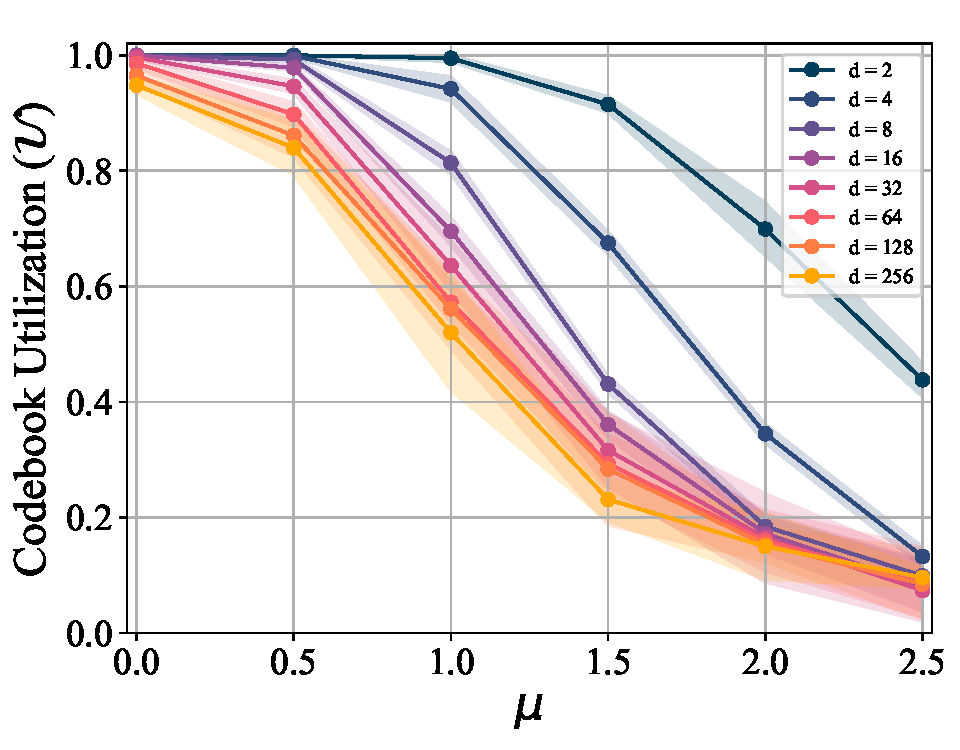
\includegraphics[width=0.16\textwidth]{figs/quantitative_analyses/gaussian_distribution/FeatureDim_mean_Utili.pdf}
    }
    \hspace{-0.39cm}
    \subfloat[$\cU$ {w.r.t.} $N$]{
        \label{fig:gaussian_featuresize_mean_utilization}
        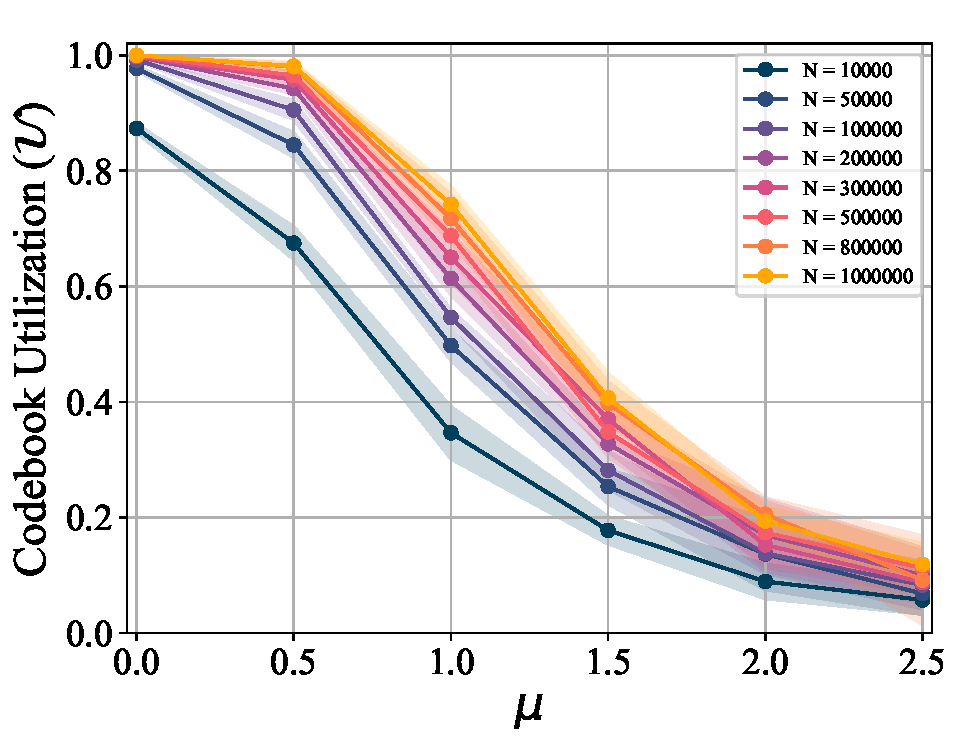
\includegraphics[width=0.16\textwidth]{figs/quantitative_analyses/gaussian_distribution/FeatureSize_mean_Utili.pdf}
    }
    \hspace{-0.39cm}
    \subfloat[$\cU$ {w.r.t.} $K$]{ 
        \label{fig:gaussian_codebooksize_sigma_utilization}  
        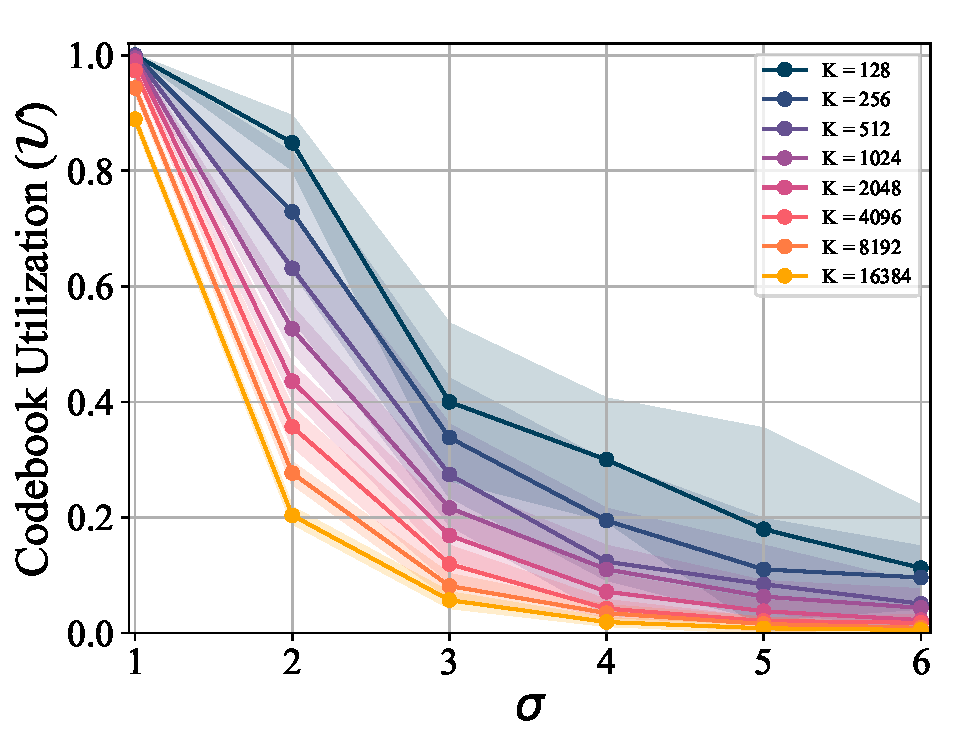
\includegraphics[width=0.16\textwidth]{figs/quantitative_analyses/gaussian_distribution/CodebookSize_Var_Util.pdf}
    }
    \hspace{-0.39cm}
    \subfloat[$\cU$ {w.r.t.} $d$]{
        \label{fig:gaussian_featuredim_sigma_utilization}
        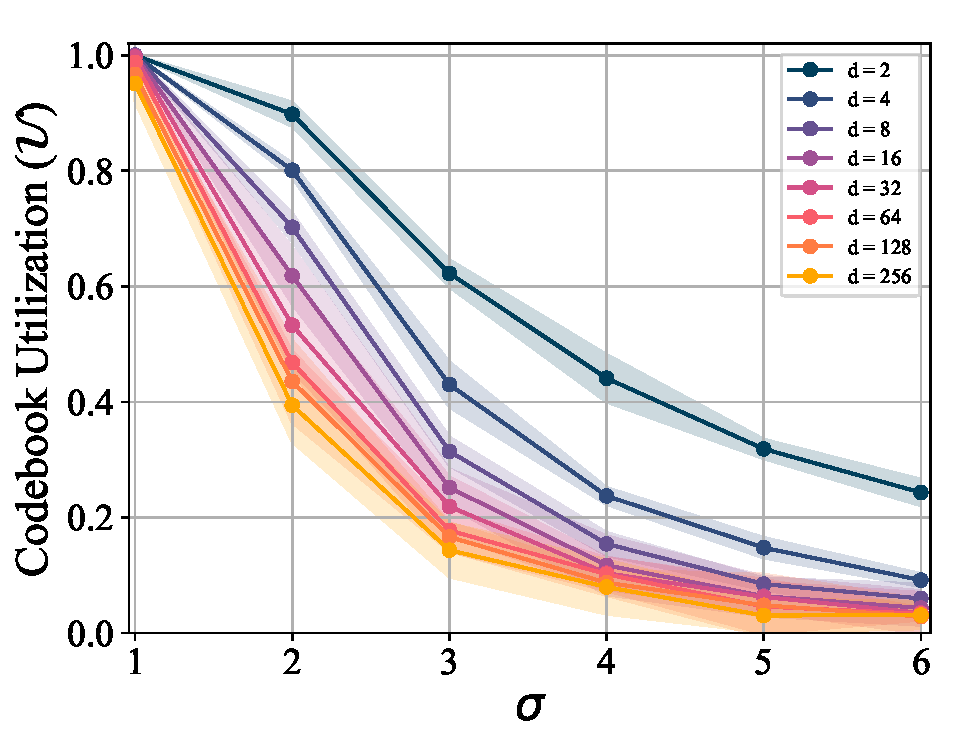
\includegraphics[width=0.16\textwidth]{figs/quantitative_analyses/gaussian_distribution/FeatureDim_Var_Util.pdf}
    }
    \hspace{-0.39cm}
    \subfloat[$\cU$ {w.r.t.} $N$]{
        \label{fig:gaussian_featuresize_sigma_utilization}
        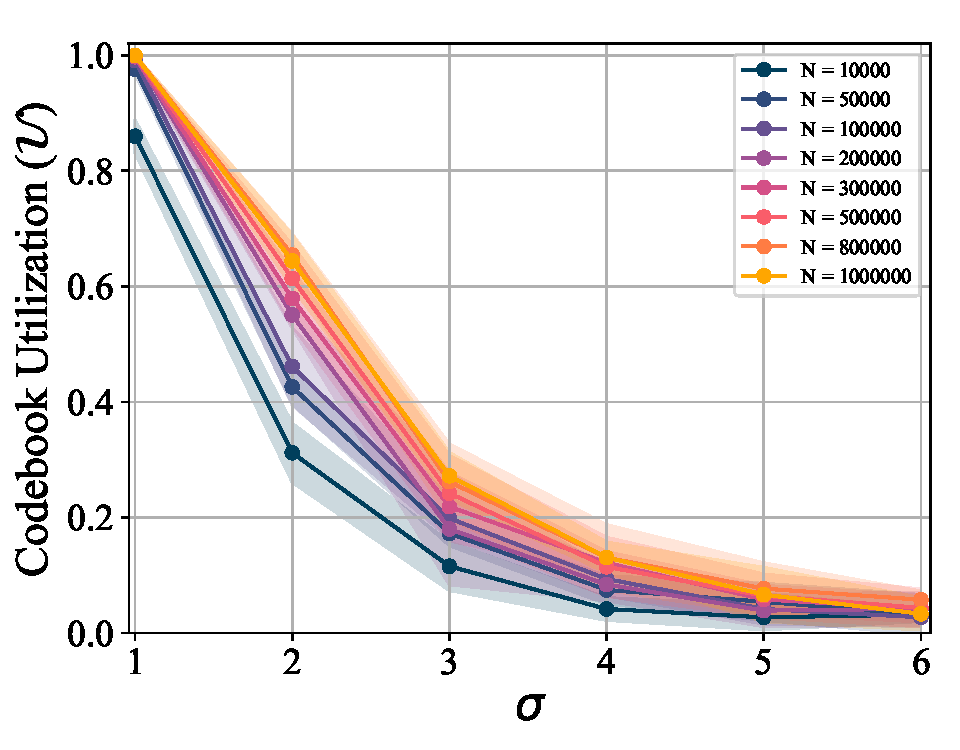
\includegraphics[width=0.16\textwidth]{figs/quantitative_analyses/gaussian_distribution/FeatureSize_Var_Util.pdf}
    }

    %%%%%%%%%%%%%%%%%%%%% Row 3: Codebook Perplexity %%%%%%%%%%%%%%%%%%%%%
    \subfloat[$\mathcal{C}$ {w.r.t.} $K$]{ 
        \label{fig:gaussian_codebooksize_mean_perplexity}  
        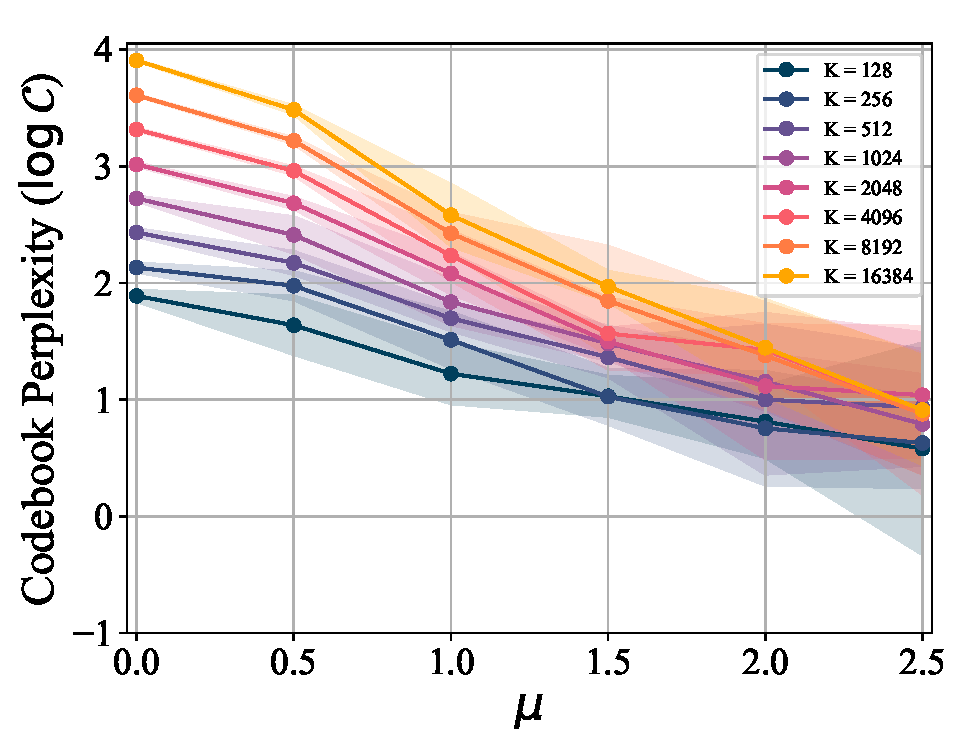
\includegraphics[width=0.16\textwidth]{figs/quantitative_analyses/gaussian_distribution/CodebookSize_mean_ppl.pdf}
    }
    \hspace{-0.39cm}
    \subfloat[$\mathcal{C}$ {w.r.t.} $d$]{
        \label{fig:gaussian_featuredim_mean_perplexity}
        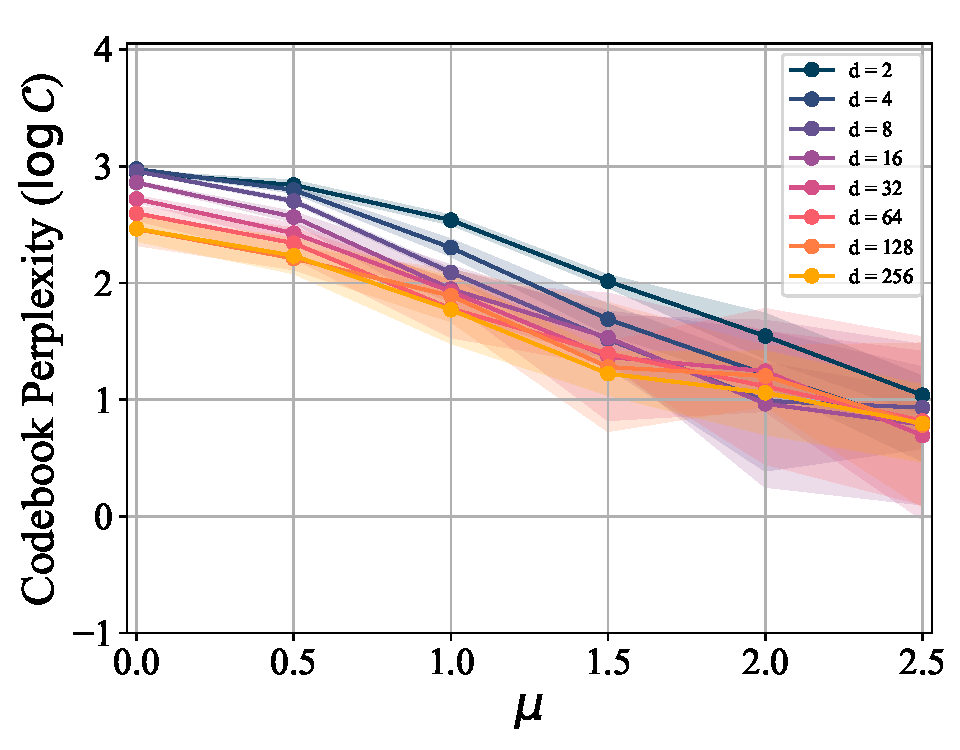
\includegraphics[width=0.16\textwidth]{figs/quantitative_analyses/gaussian_distribution/FeatureDim_mean_ppl.pdf}
    }
    \hspace{-0.39cm}
    \subfloat[$\mathcal{C}$ {w.r.t.} $N$]{
        \label{fig:gaussian_featuresize_mean_perplexity}
        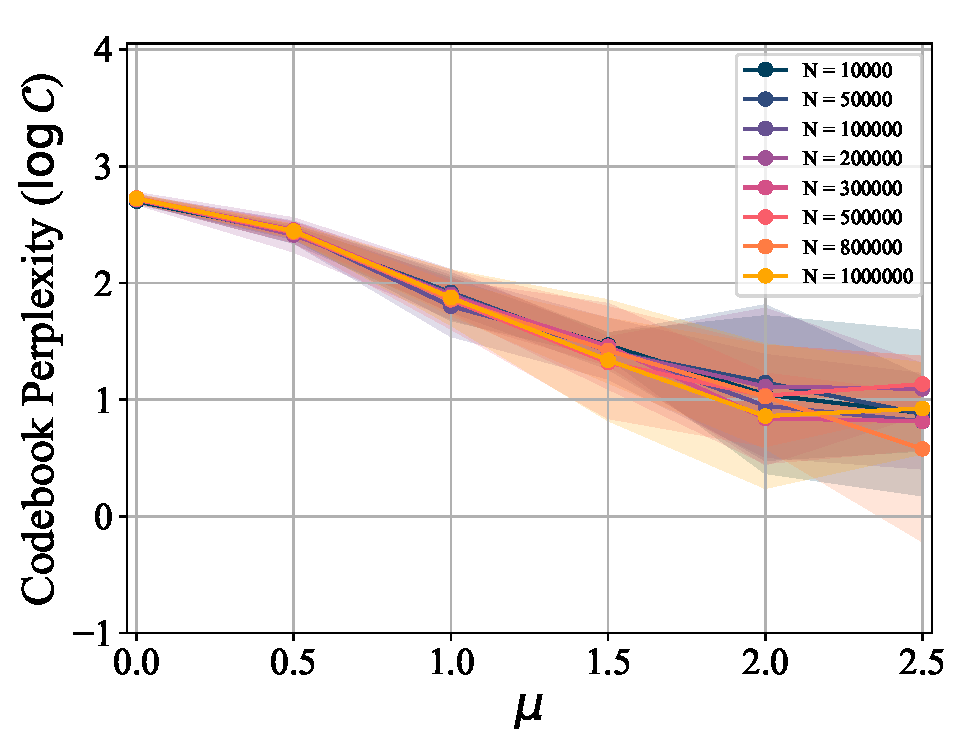
\includegraphics[width=0.16\textwidth]{figs/quantitative_analyses/gaussian_distribution/FeatureSize_mean_ppl.pdf}
    }
    \hspace{-0.39cm}
    \subfloat[$\mathcal{C}$ {w.r.t.} $K$]{ 
        \label{fig:gaussian_codebooksize_sigma_perplexity}  
        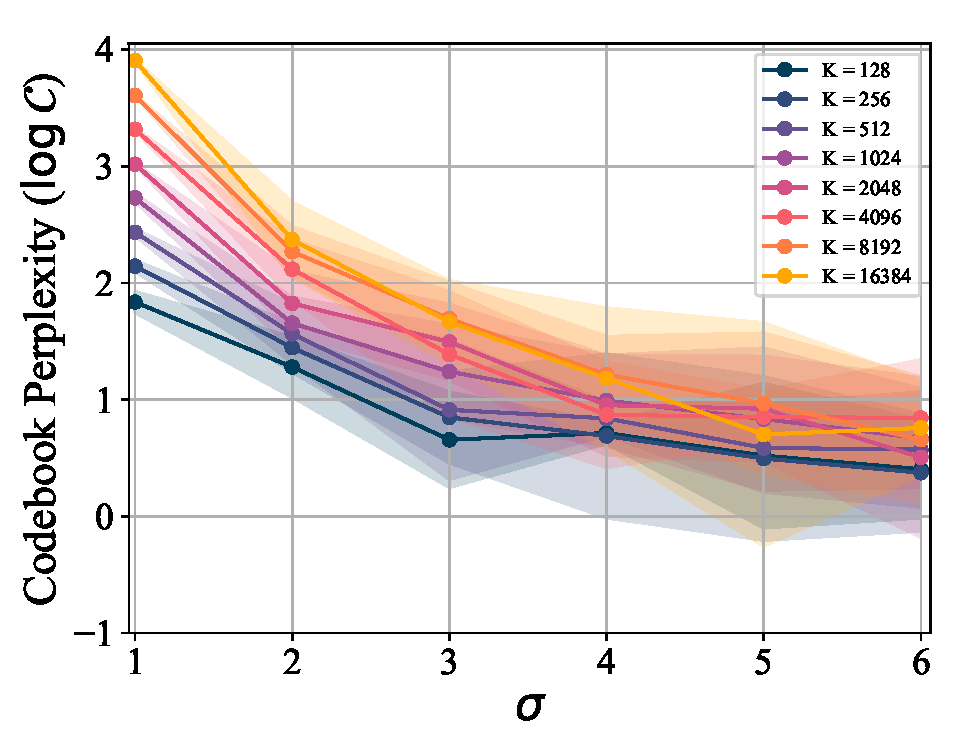
\includegraphics[width=0.16\textwidth]{figs/quantitative_analyses/gaussian_distribution/CodebookSize_Var_ppl.pdf}
    }
    \hspace{-0.39cm}
    \subfloat[$\mathcal{C}$ {w.r.t.} $d$]{
        \label{fig:gaussian_featuredim_sigma_perplexity}
        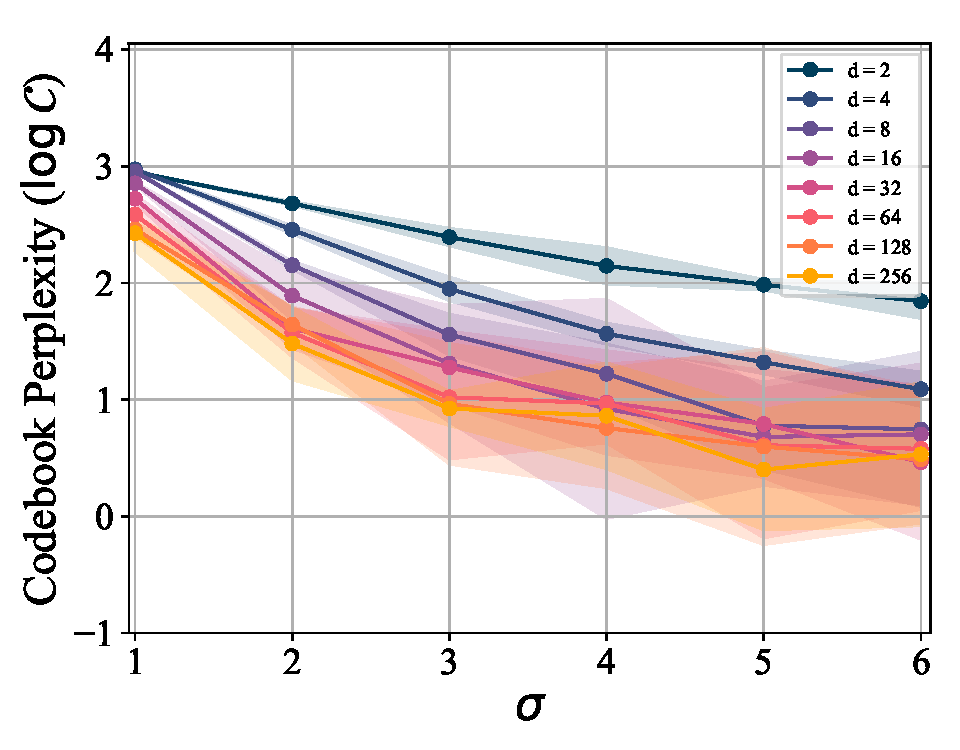
\includegraphics[width=0.16\textwidth]{figs/quantitative_analyses/gaussian_distribution/FeatureDim_Var_ppl.pdf}
    }
    \hspace{-0.39cm}
    \subfloat[$\mathcal{C}$ {w.r.t.} $N$]{
        \label{fig:gaussian_featuresize_sigma_perplexity}
        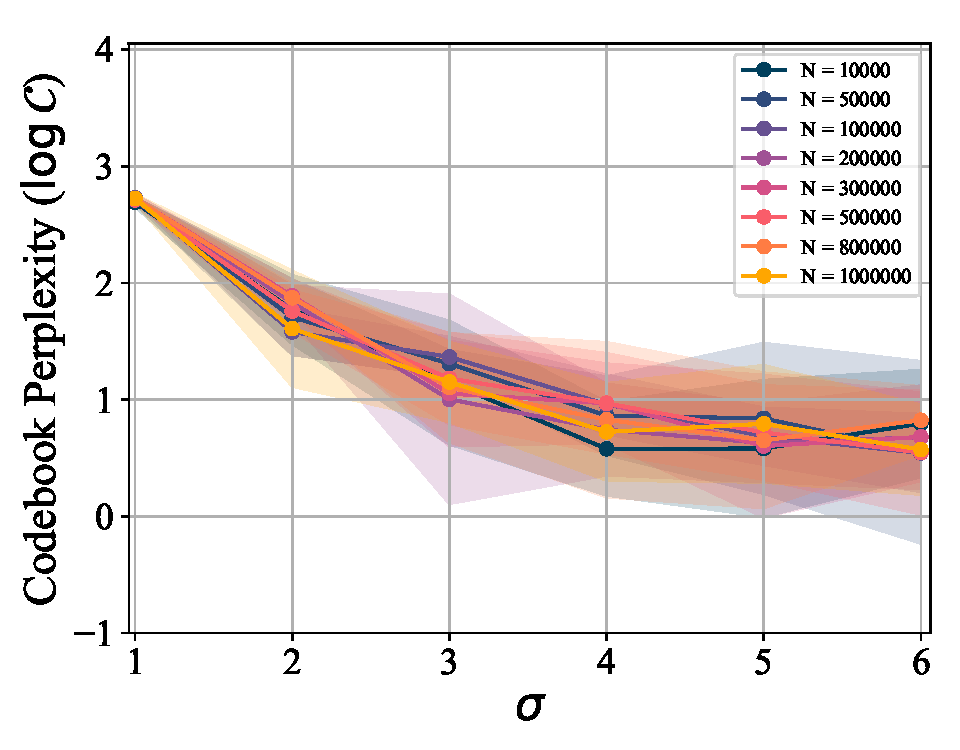
\includegraphics[width=0.16\textwidth]{figs/quantitative_analyses/gaussian_distribution/FeatureSize_Var_ppl.pdf}
    }
    \vspace{-1ex}
    \caption{\small{Quantitative analyses of the criterion triple when $\mathcal{P}_A$ and $\mathcal{P}_B$ are Gaussian distributions.}}
    \label{fig:quantitative analysis gaussian distribution}
    \vspace{-4ex}
\end{figure*}

\begin{figure*}[!t]
    \vspace{-1ex}
	\centering

    %%%%%%%%%%%%%%%%%%%%% Quantization Error %%%%%%%%%%%%%
	\subfloat[$\cE$ {w.r.t.} $K$]{ 
		\label{fig:uniform_codebooksize_mean_error}  
		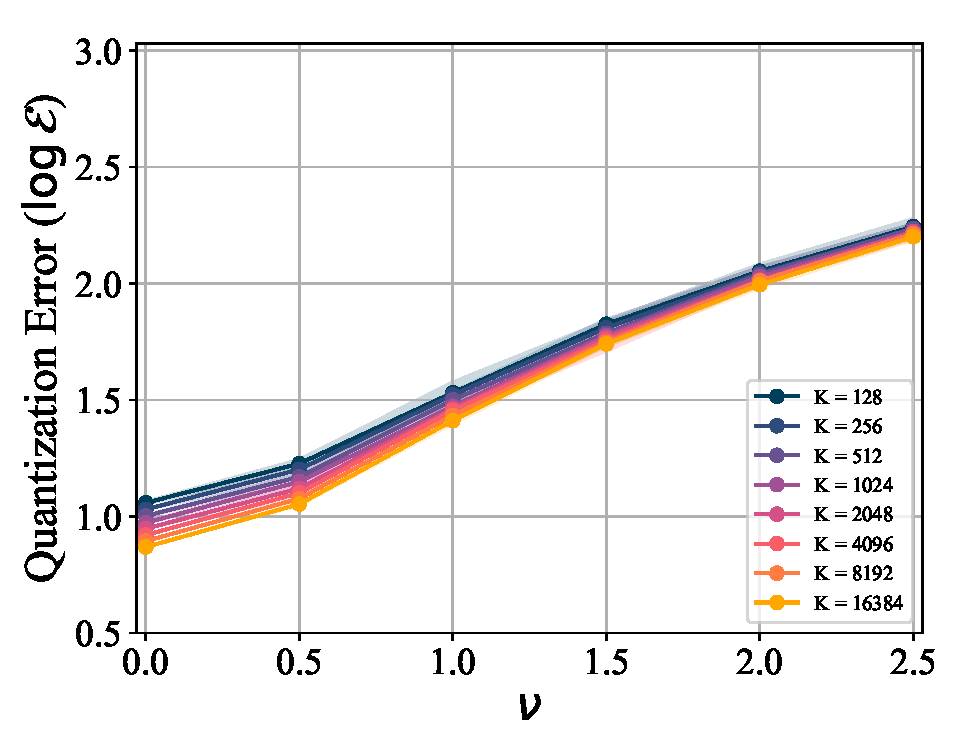
\includegraphics[width=0.16\textwidth]{figs/quantitative_analyses/uniform_distribution/Uniform_CodebookSize_mean_Quant.pdf}
    }
    \hspace{-0.39cm}
	\subfloat[$\cE$ {w.r.t.} $d$]{
		\label{fig:uniform_featuredim_mean_error}
		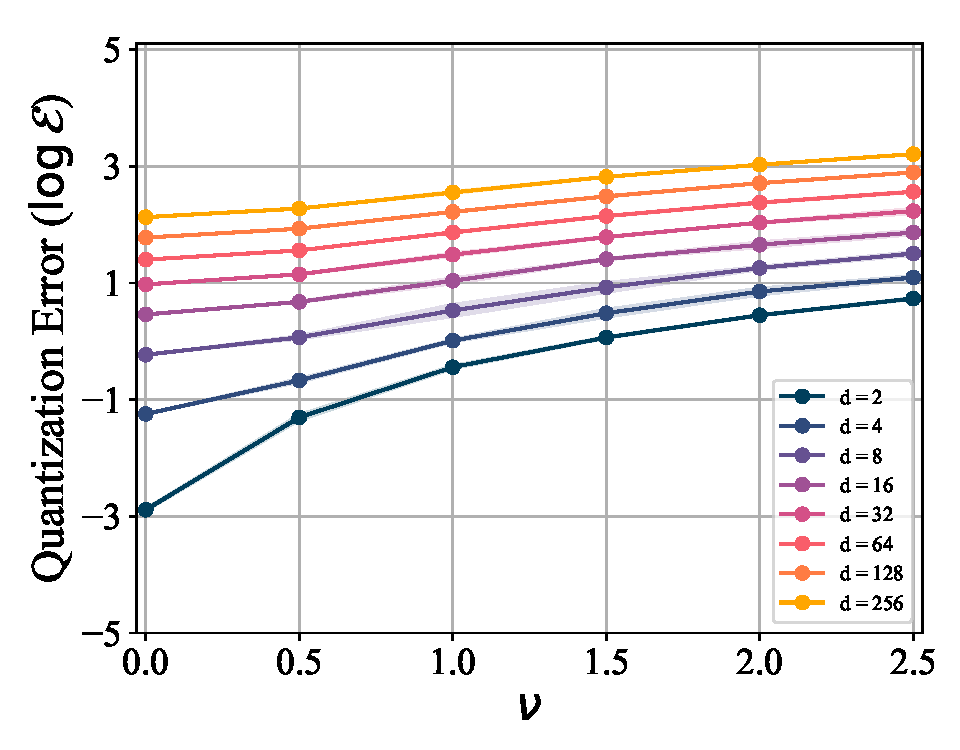
\includegraphics[width=0.16\textwidth]{figs/quantitative_analyses/uniform_distribution/Uniform_FeatureDim_mean_Quant.pdf}
	}
    \hspace{-0.39cm}
	\subfloat[$\cE$ {w.r.t.} $N$]{
		\label{fig:uniform_featuresize_mean_error}
		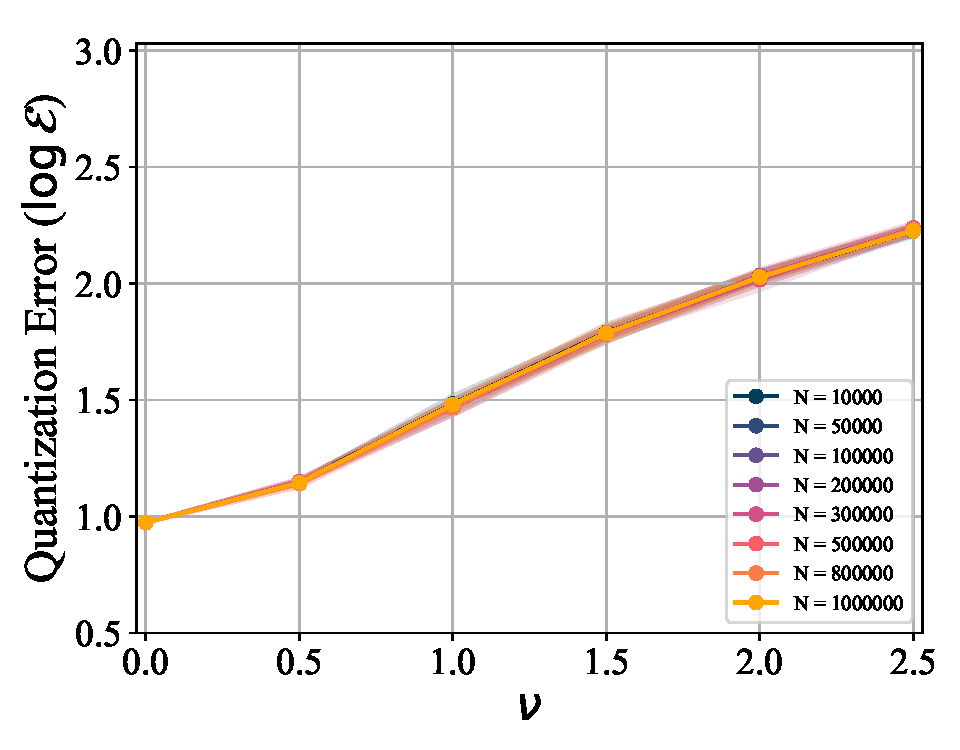
\includegraphics[width=0.16\textwidth]{figs/quantitative_analyses/uniform_distribution/Uniform_FeatureSize_mean_Quant.pdf}
	}
    \hspace{-0.39cm}
	\subfloat[$\cE$ {w.r.t.} $K$]{ 
		\label{fig:uniform_codebooksize_sigma_error}  
		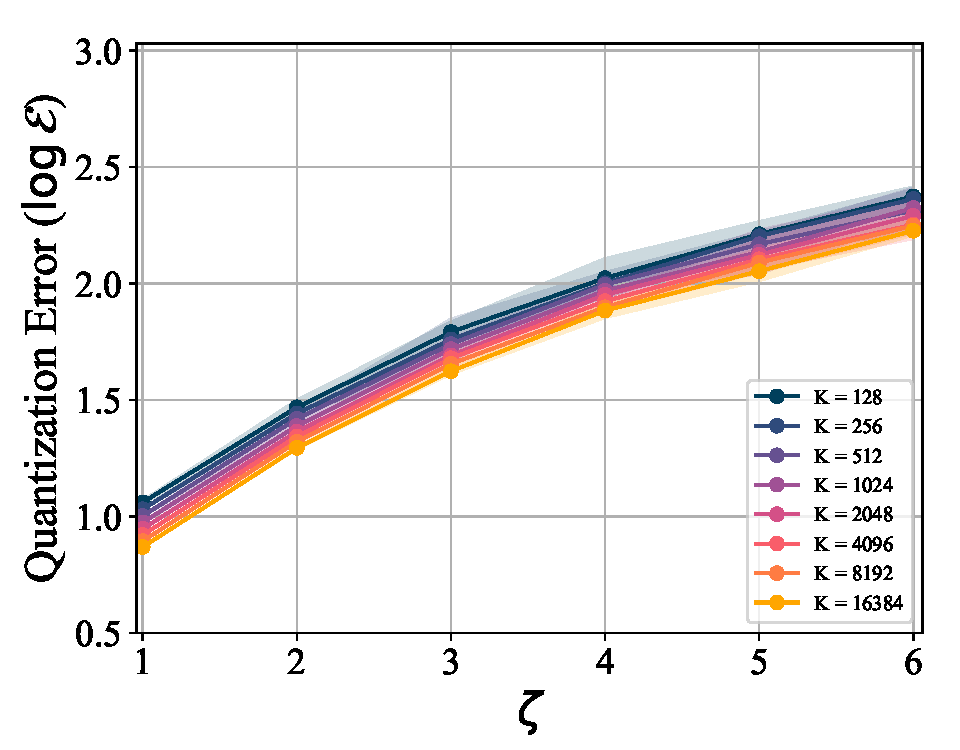
\includegraphics[width=0.16\textwidth]{figs/quantitative_analyses/uniform_distribution/Uniform_CodebookSize_Var_Quant.pdf}
	}
    \hspace{-0.39cm}
	\subfloat[$\cE$ {w.r.t.} $d$]{
		\label{fig:uniform_featuredim_sigma_error}
		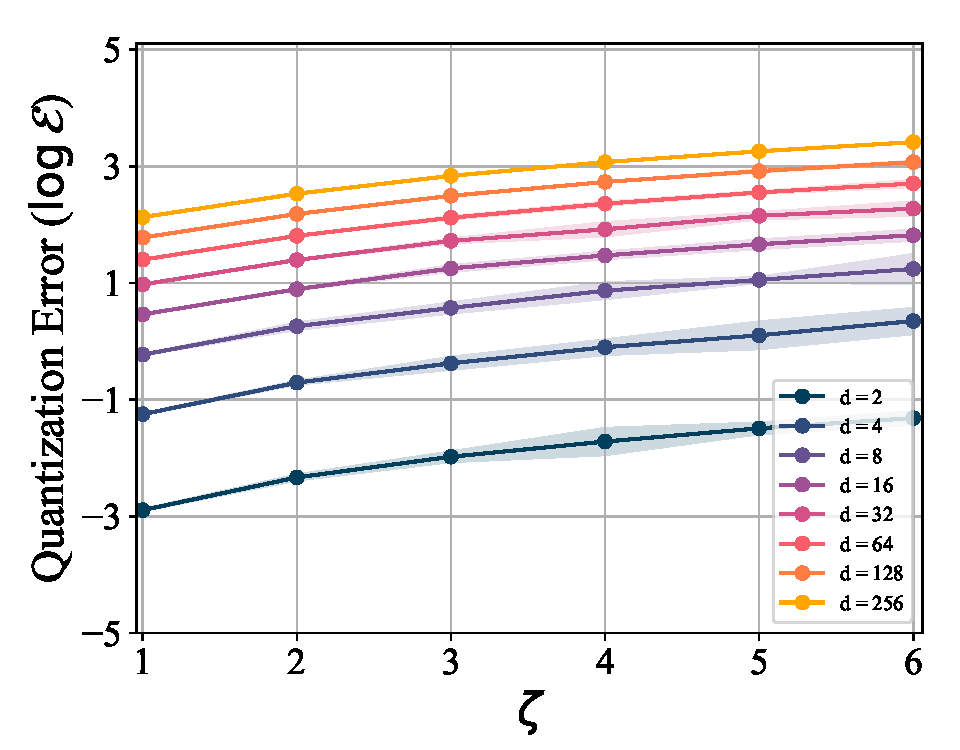
\includegraphics[width=0.16\textwidth]{figs/quantitative_analyses/uniform_distribution/Uniform_FeatureDim_Var_Quant.pdf}
	}
    \hspace{-0.39cm}
	\subfloat[$\cE$ {w.r.t.} $N$]{
		\label{fig:uniform_featuresize_sigma_error}
		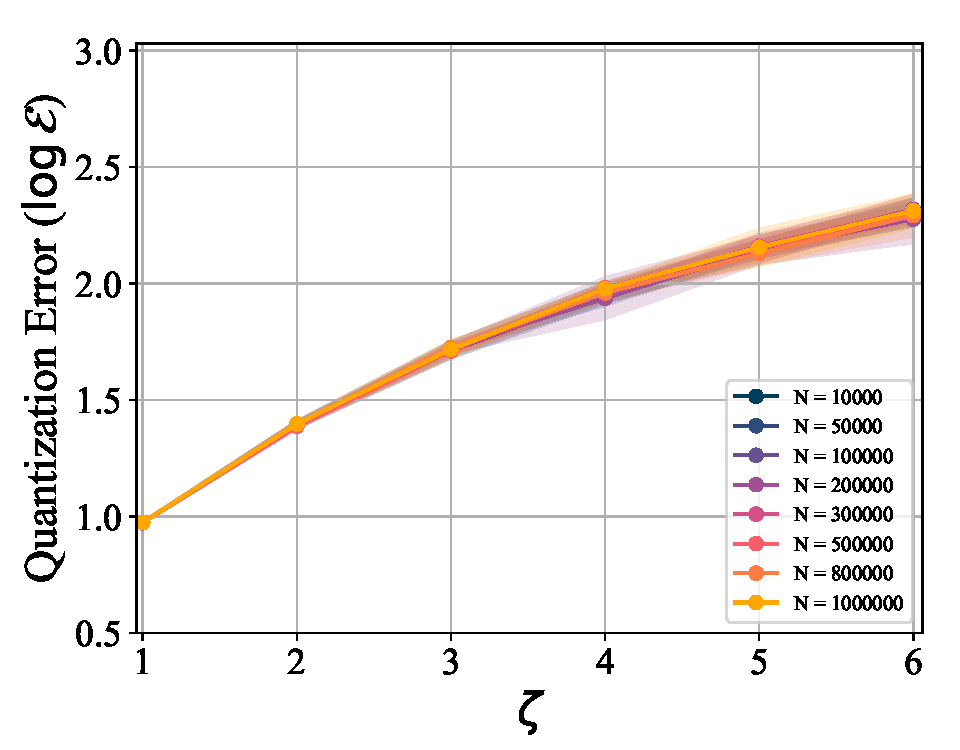
\includegraphics[width=0.16\textwidth]{figs/quantitative_analyses/uniform_distribution/Uniform_FeatureSize_Var_Quant.pdf}
	}

    %\\[-1ex]

    %%%%%%%%%%%%%%%%%%%%%%%%%%% Codebook Utilization %%%%%%%%%%%%%%%%%%%%%%
	\subfloat[$\cU$ {w.r.t.} $K$]{ 
        \label{fig:uniform_codebooksize_mean_utilization}  
		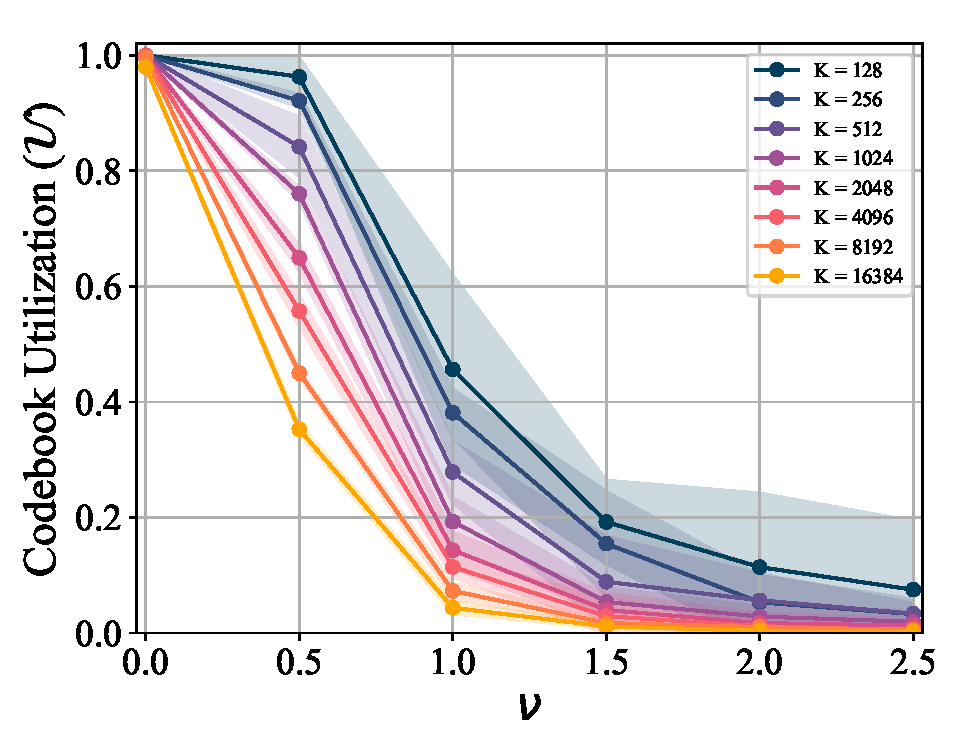
\includegraphics[width=0.16\textwidth]{figs/quantitative_analyses/uniform_distribution/Uniform_CodebookSize_mean_Utili.pdf}
    }
	\hspace{-0.39cm}
	\subfloat[$\cU$ {w.r.t.} $d$]{
        \label{fig:uniform_featuredim_mean_utilization}
		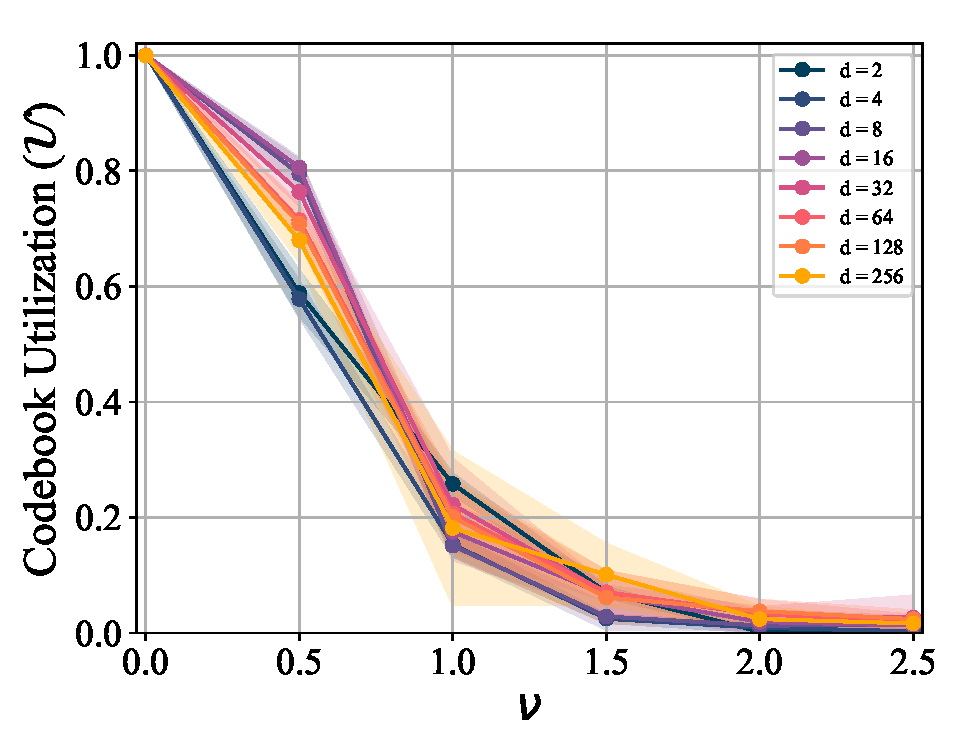
\includegraphics[width=0.16\textwidth]{figs/quantitative_analyses/uniform_distribution/Uniform_FeatureDim_mean_Utili.pdf}
	}
	\hspace{-0.39cm}
	\subfloat[$\cU$ {w.r.t.} $N$]{
        \label{fig:uniform_featuresize_mean_utilization}
		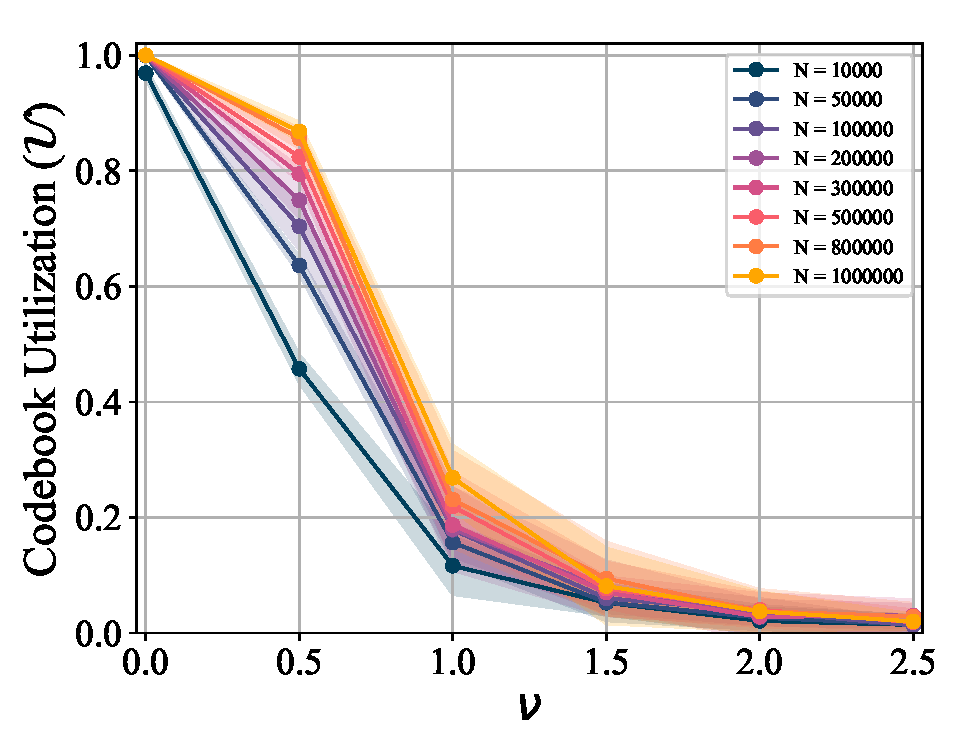
\includegraphics[width=0.16\textwidth]{figs/quantitative_analyses/uniform_distribution/Uniform_FeatureSize_mean_Utili.pdf}
	}
    \hspace{-0.39cm}
	\subfloat[$\cU$ {w.r.t.} $K$]{ 
        \label{fig:uniform_codebooksize_sigma_utilization}  
		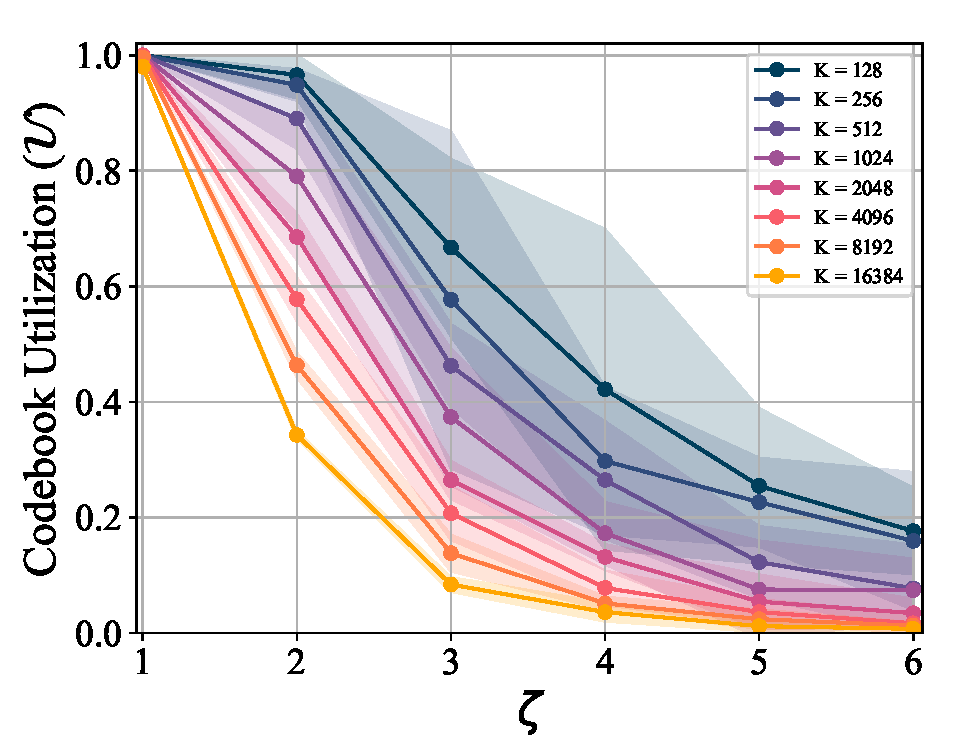
\includegraphics[width=0.16\textwidth]{figs/quantitative_analyses/uniform_distribution/Uniform_CodebookSize_Var_Util.pdf}
	}
    \hspace{-0.39cm}
	\subfloat[$\cU$ {w.r.t.} $d$]{
        \label{fig:uniform_featuredim_sigma_utilization}
		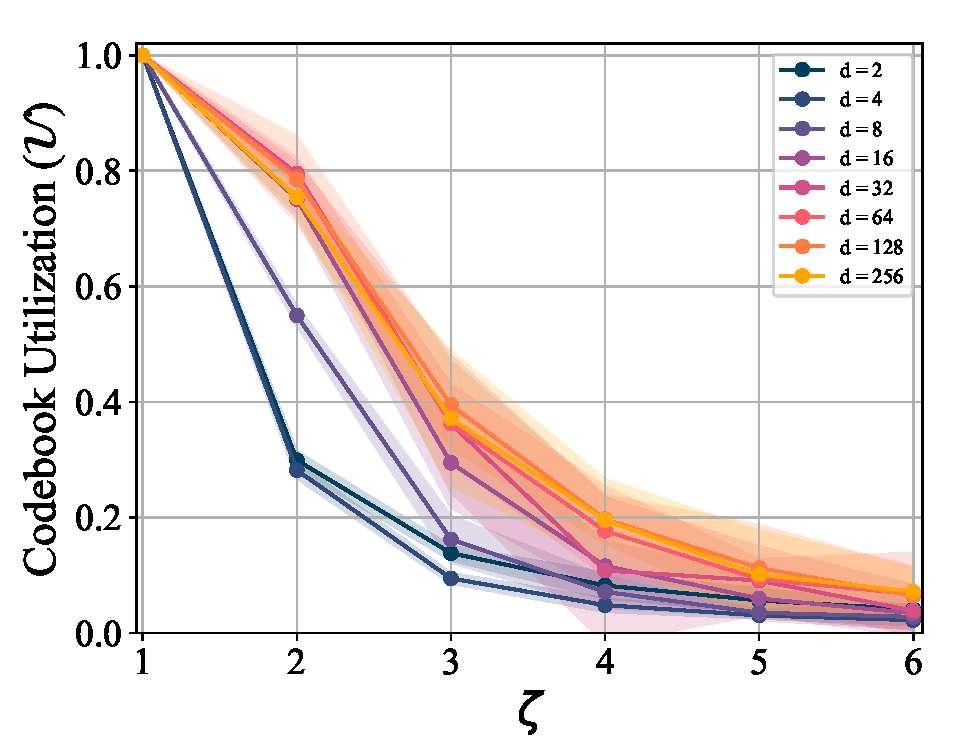
\includegraphics[width=0.16\textwidth]{figs/quantitative_analyses/uniform_distribution/Uniform_FeatureDim_Var_Util.pdf}
	}
    \hspace{-0.39cm}
	\subfloat[$\cU$ {w.r.t.} $N$]{
        \label{fig:uniform_featuresize_sigma_utilization}
		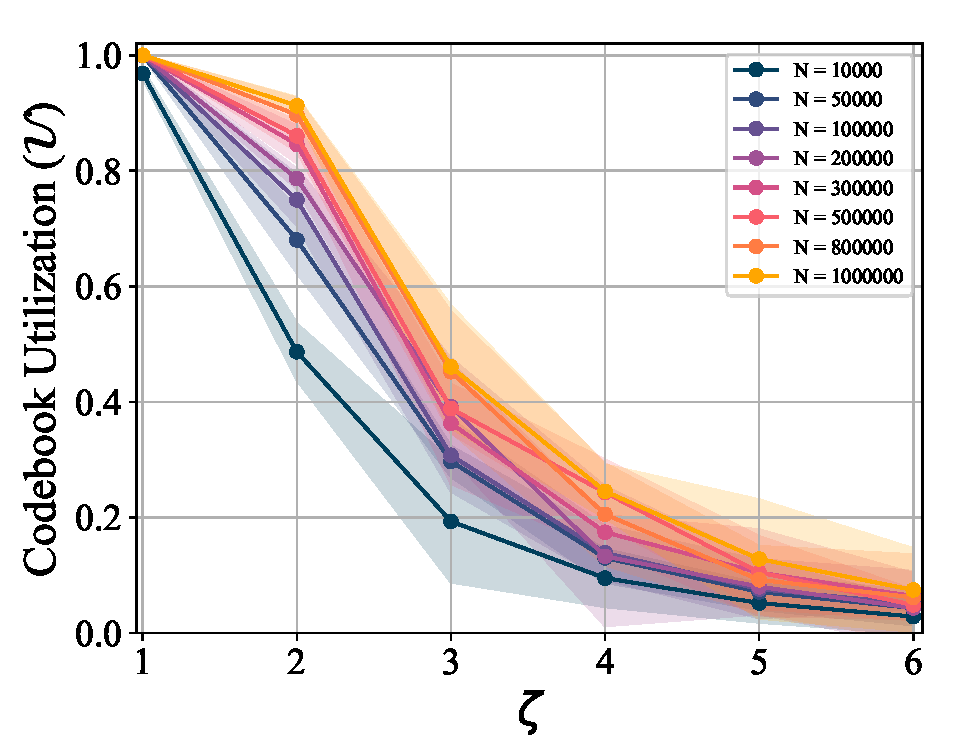
\includegraphics[width=0.16\textwidth]{figs/quantitative_analyses/uniform_distribution/Uniform_FeatureSize_Var_Util.pdf}
	}

    %\\[-1ex]

    %%%%%%%%%%%%%%%%%%%%%%%%%% Codebook Perplexity %%%%%%%%%%%%%%%%%%%%%%%%%
	\subfloat[$\mathcal{C}$ {w.r.t.} $K$]{ 
        \label{fig:uniform_codebooksize_mean_perplexity}  
		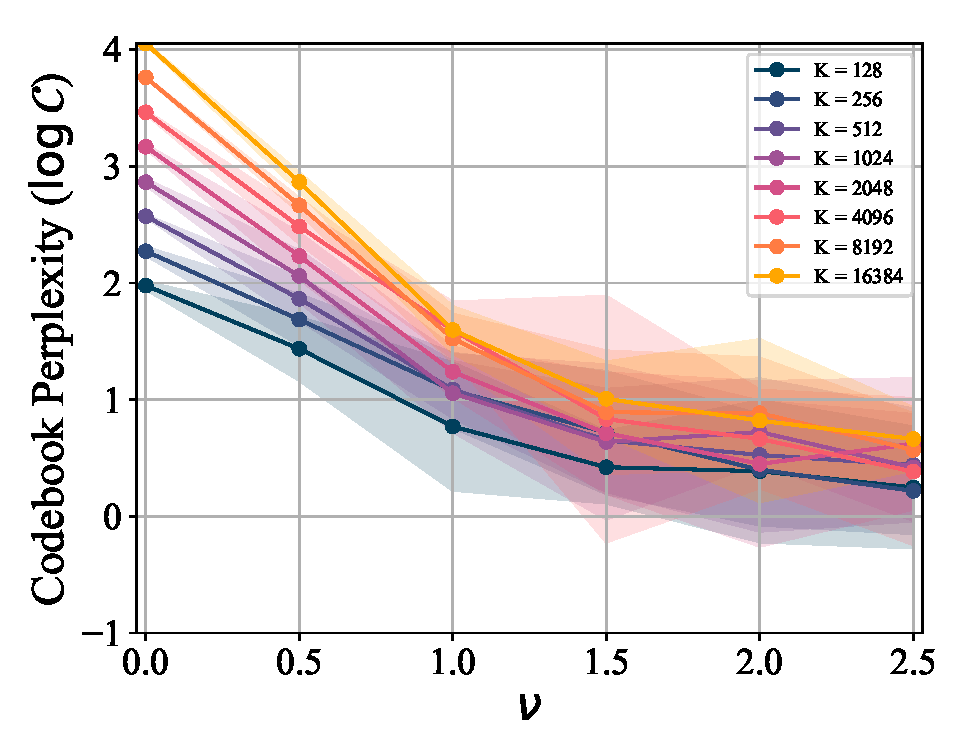
\includegraphics[width=0.16\textwidth]{figs/quantitative_analyses/uniform_distribution/Uniform_CodebookSize_mean_ppl.pdf}
    }
	\hspace{-0.39cm}
	\subfloat[$\mathcal{C}$ {w.r.t.} $d$]{
        \label{fig:uniform_featuredim_mean_perplexity}
		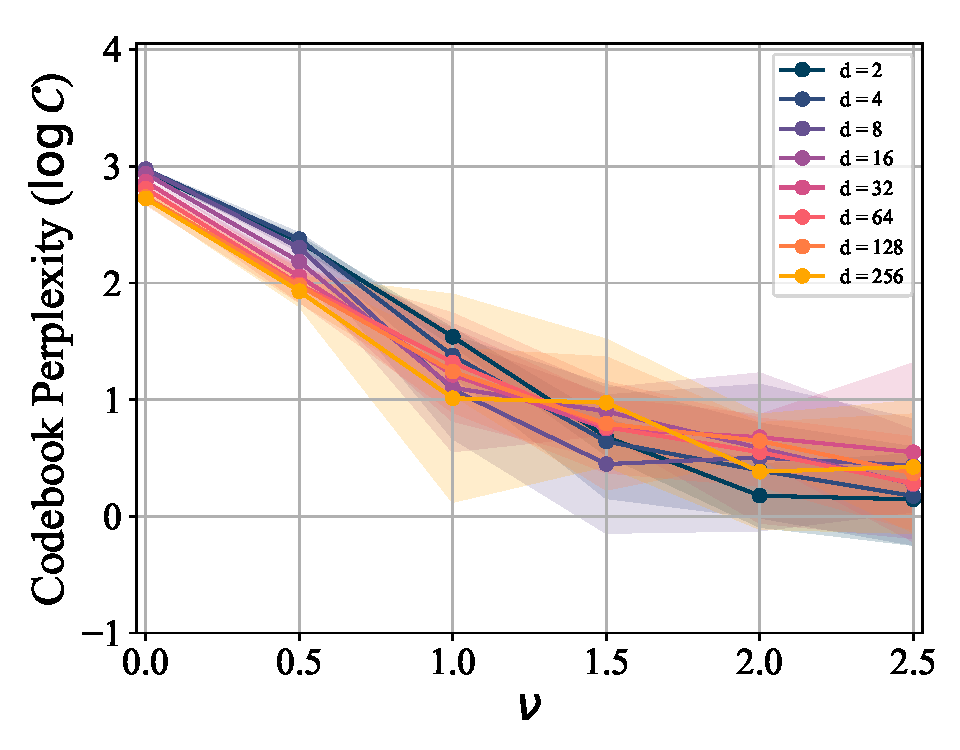
\includegraphics[width=0.16\textwidth]{figs/quantitative_analyses/uniform_distribution/Uniform_FeatureDim_mean_ppl.pdf}
	}
	\hspace{-0.39cm}
	\subfloat[$\mathcal{C}$ {w.r.t.} $N$]{
        \label{fig:uniform_featuresize_mean_perplexity}
		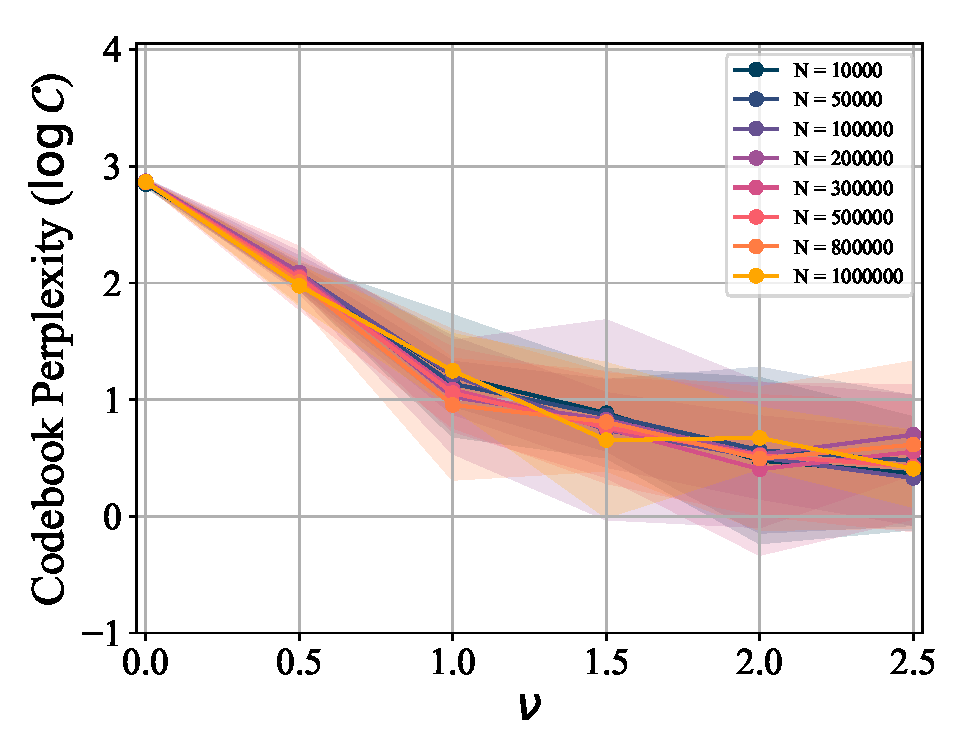
\includegraphics[width=0.16\textwidth]{figs/quantitative_analyses/uniform_distribution/Uniform_FeatureSize_mean_ppl.pdf}
	}
    \hspace{-0.39cm}
	\subfloat[$\mathcal{C}$ {w.r.t.} $K$]{ 
        \label{fig:uniform_codebooksize_sigma_perplexity}  
		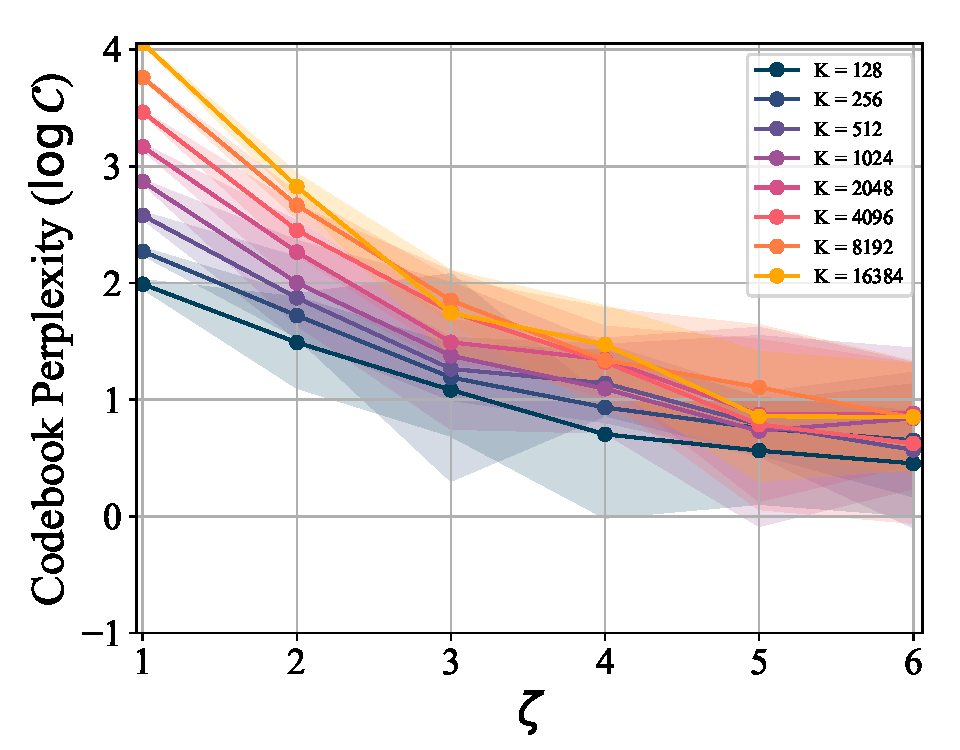
\includegraphics[width=0.16\textwidth]{figs/quantitative_analyses/uniform_distribution/Uniform_CodebookSize_Var_ppl.pdf}
	}
    \hspace{-0.39cm}
	\subfloat[$\mathcal{C}$ {w.r.t.} $d$]{
        \label{fig:uniform_featuredim_sigma_perplexity}
		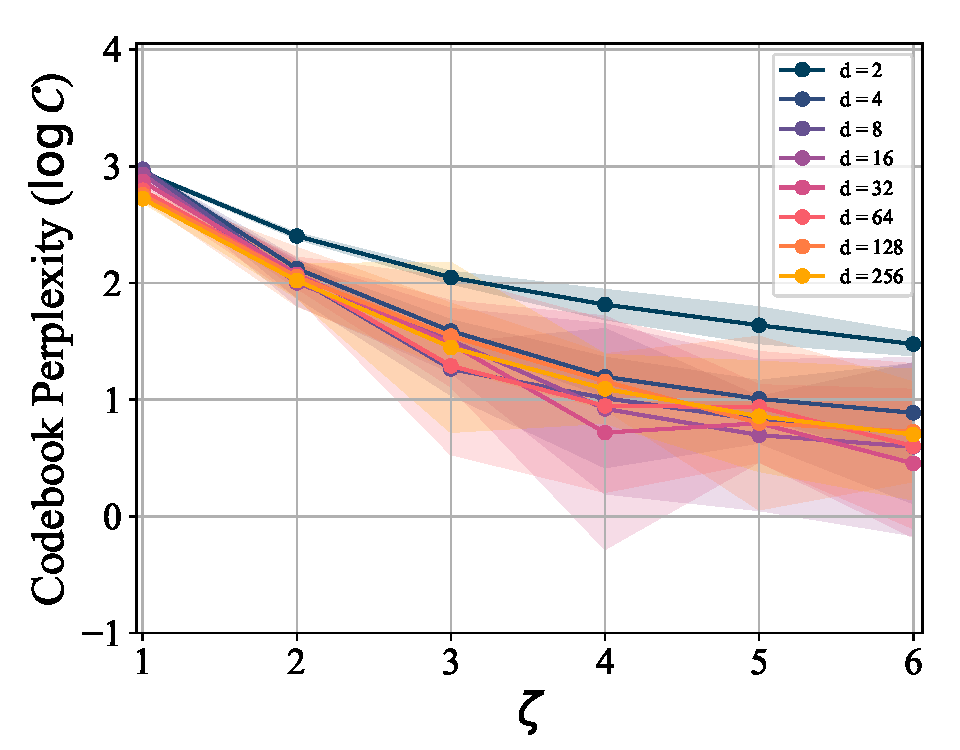
\includegraphics[width=0.16\textwidth]{figs/quantitative_analyses/uniform_distribution/Uniform_FeatureDim_Var_ppl.pdf}
	}
    \hspace{-0.39cm}
	\subfloat[$\mathcal{C}$ {w.r.t.} $N$]{
        \label{fig:uniform_featuresize_sigma_perplexity}
		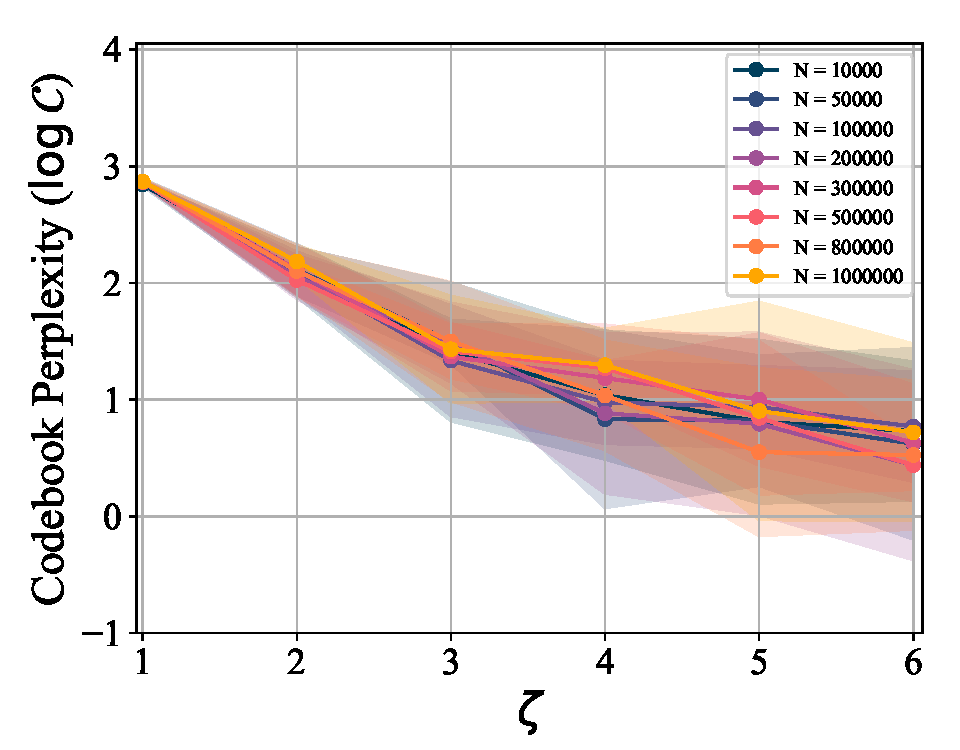
\includegraphics[width=0.16\textwidth]{figs/quantitative_analyses/uniform_distribution/Uniform_FeatureSize_Var_ppl.pdf}
	}

    \vspace{-1ex}
	\caption{Quantitative analyses of the criterion triple when $\mathcal{P}_A$ and $\mathcal{P}_B$ are uniform distributions.}
    \vspace{-2ex}
	\label{fig:quantitative analysis uniform distribution}
\end{figure*}


\iffalse
\begin{figure*}[!t]
    \vspace{-1ex}
	\centering
    %%%%%%%%%%%%%%%%%%%%% Quantization Error %%%%%%%%%%%%%
	\subfloat[$\cE$ {w.r.t.} $K$]{ 
		\label{fig:uniform_codebooksize_mean_error}  
		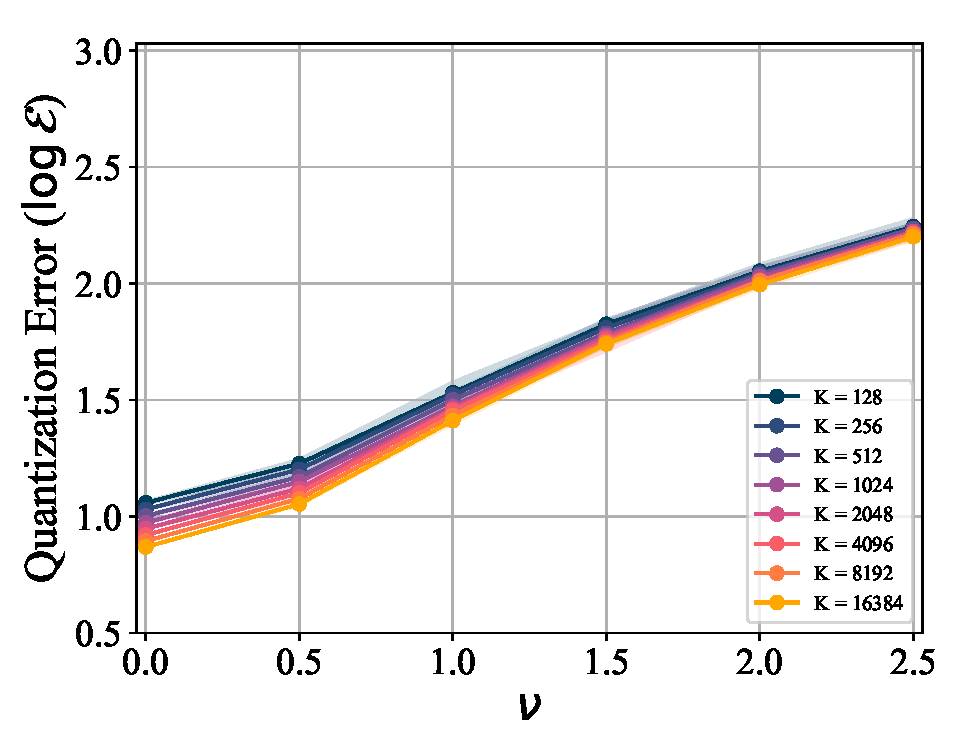
\includegraphics[width=0.16\textwidth]{figs/quantitative_analyses/uniform_distribution/Uniform_CodebookSize_mean_Quant.pdf}
        }
    \hspace{-0.39cm}
	\subfloat[$\cE$ {w.r.t.} $d$]{
		\label{fig:uniform_featuredim_mean_error}
		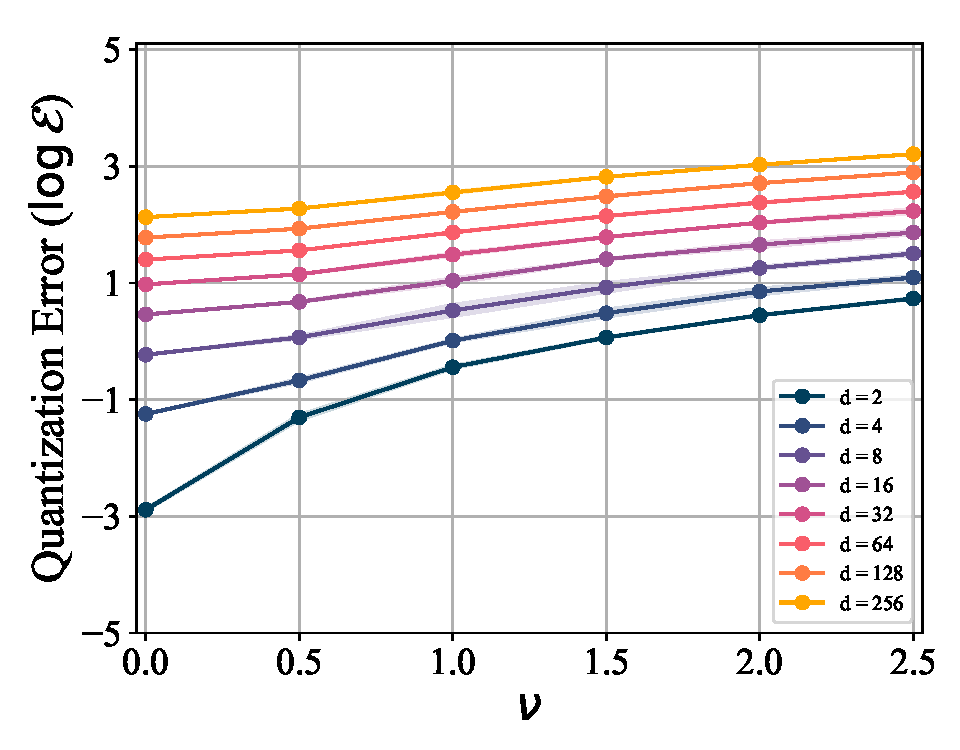
\includegraphics[width=0.16\textwidth]{figs/quantitative_analyses/uniform_distribution/Uniform_FeatureDim_mean_Quant.pdf}
	}
    \hspace{-0.39cm}
	\subfloat[$\cE$ {w.r.t.} $N$]{
		\label{fig:uniform_featuresize_mean_error}
		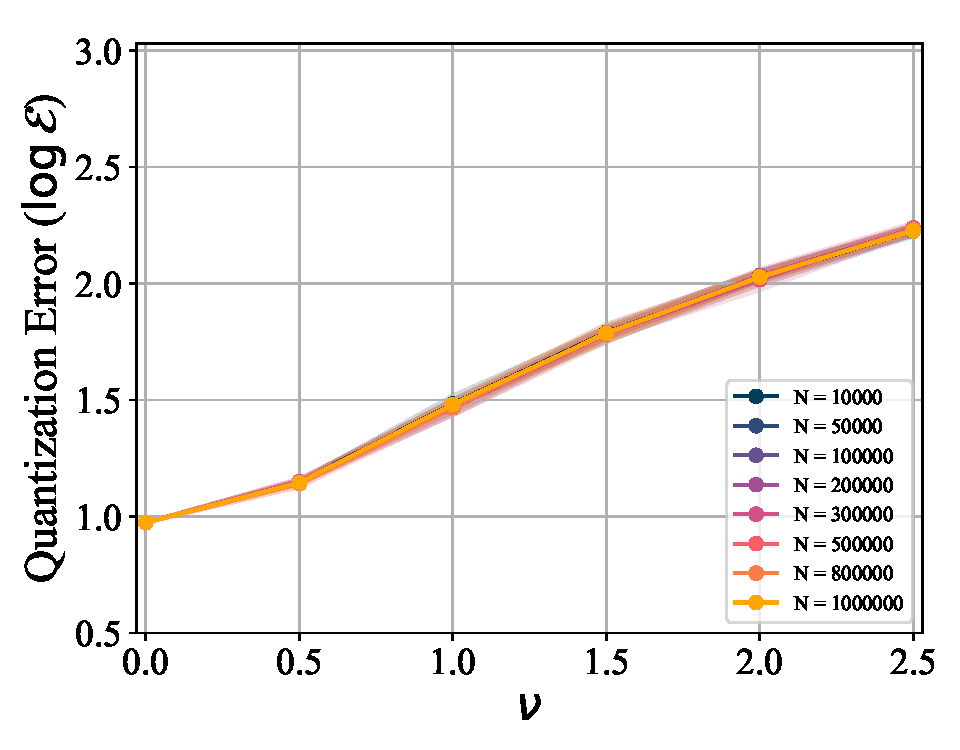
\includegraphics[width=0.16\textwidth]{figs/quantitative_analyses/uniform_distribution/Uniform_FeatureSize_mean_Quant.pdf}
	}
    \hspace{-0.39cm}
	\subfloat[$\cE$ {w.r.t.} $K$]{ 
		\label{fig:uniform_codebooksize_sigma_error}  
		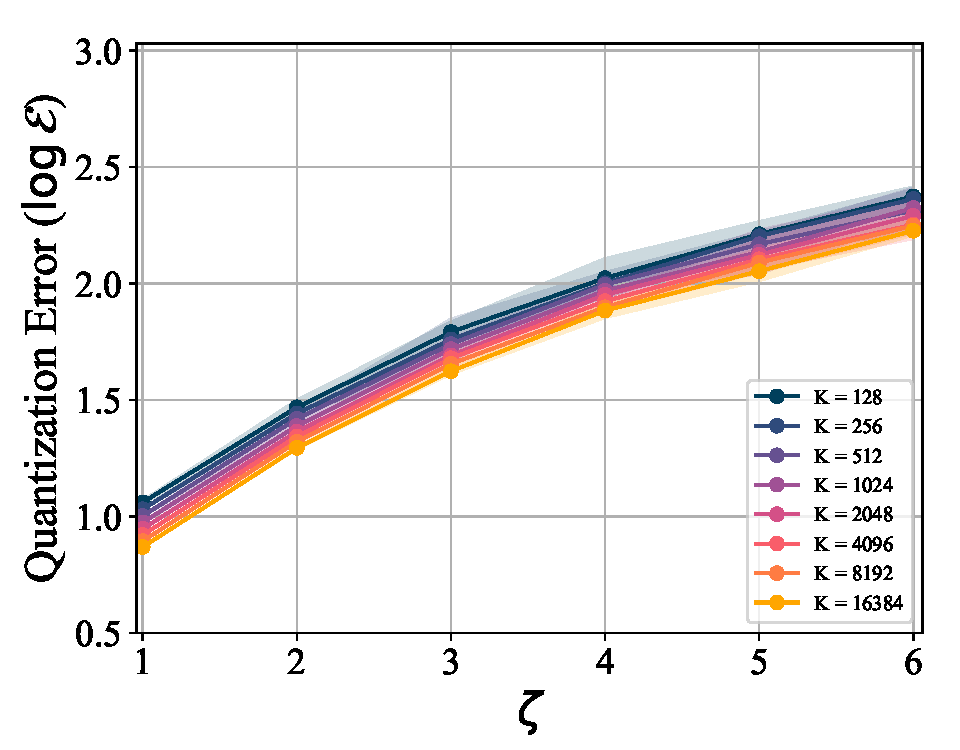
\includegraphics[width=0.16\textwidth]{figs/quantitative_analyses/uniform_distribution/Uniform_CodebookSize_Var_Quant.pdf}
	}
    \hspace{-0.39cm}
	\subfloat[$\cE$ {w.r.t.} $d$]{
		\label{fig:uniform_featuredim_sigma_error}
		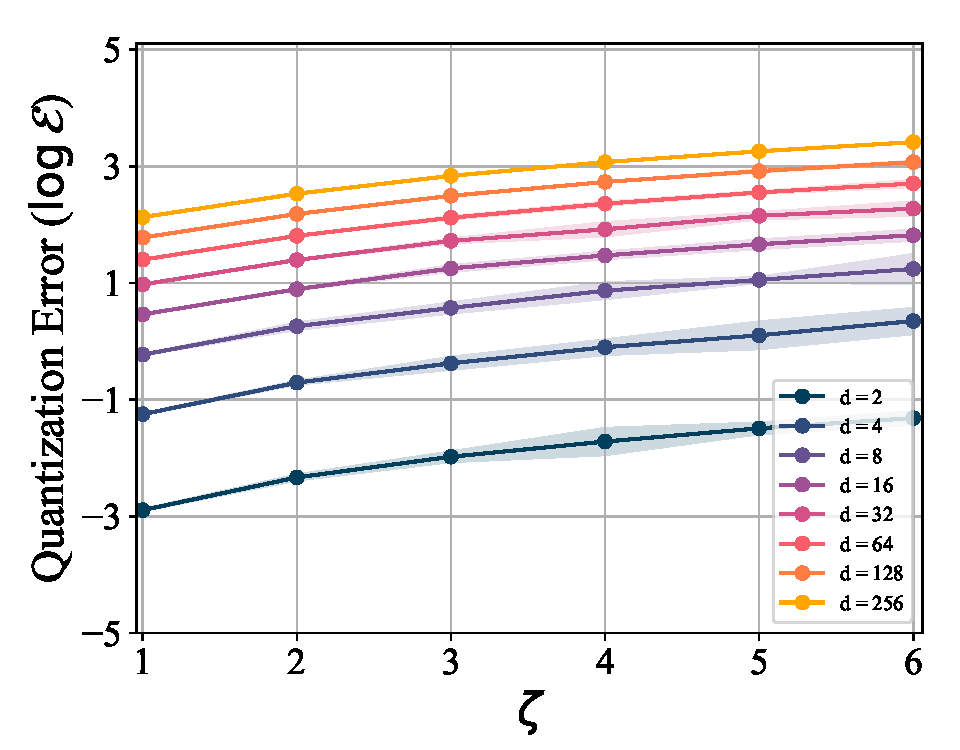
\includegraphics[width=0.16\textwidth]{figs/quantitative_analyses/uniform_distribution/Uniform_FeatureDim_Var_Quant.pdf}
	}
    \hspace{-0.39cm}
	\subfloat[$\cE$ {w.r.t.} $N$]{
		\label{fig:uniform_featuresize_sigma_error}
		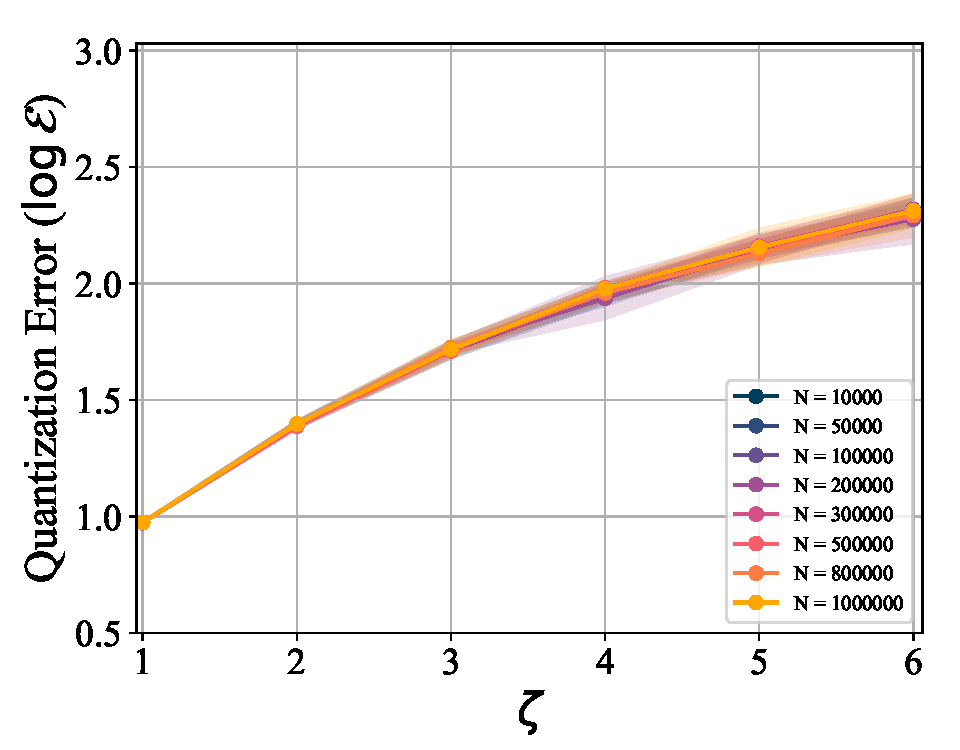
\includegraphics[width=0.16\textwidth]{figs/quantitative_analyses/uniform_distribution/Uniform_FeatureSize_Var_Quant.pdf}
	}
    %\vspace{-5pt}
    %%%%%%%%%%%%%%%%%%%%%%%%%%%Codebook Utilization%%%%%%%%%%%%%%%%%%%%%%
    %\centering
	\subfloat[$\cU$ {w.r.t.} $K$]{ \label{fig:uniform_codebooksize_mean_utilization}  
		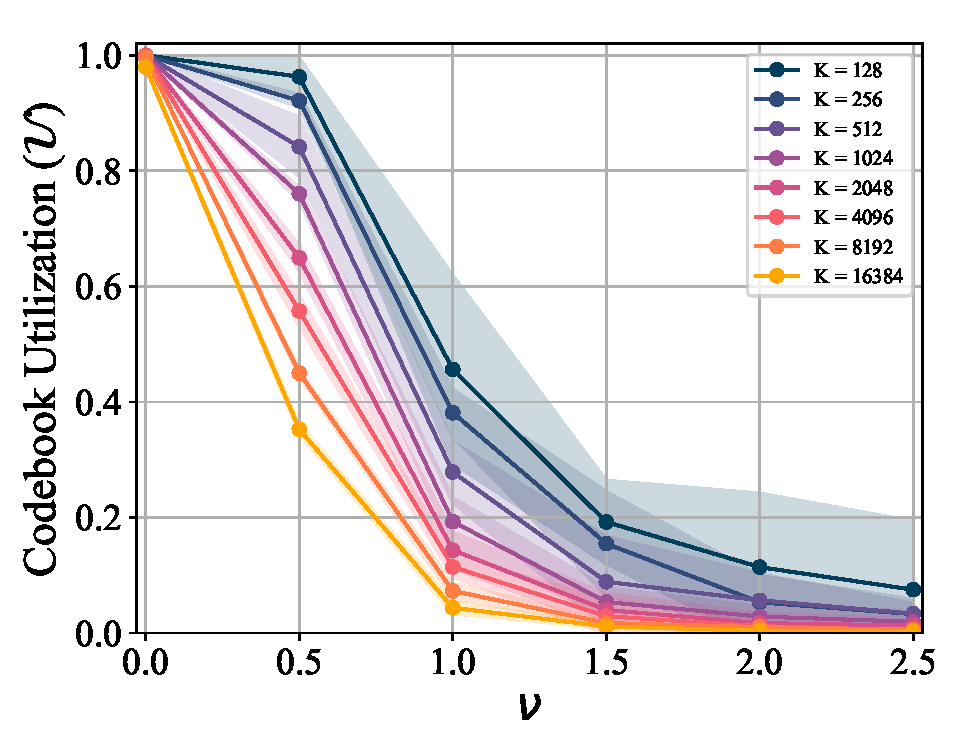
\includegraphics[width=0.16\textwidth]{figs/quantitative_analyses/uniform_distribution/Uniform_CodebookSize_mean_Utili.pdf}
        }
	\hspace{-0.39cm}
	\subfloat[$\cU$ {w.r.t.} $d$]{\label{fig:uniform_featuredim_mean_utilization}
		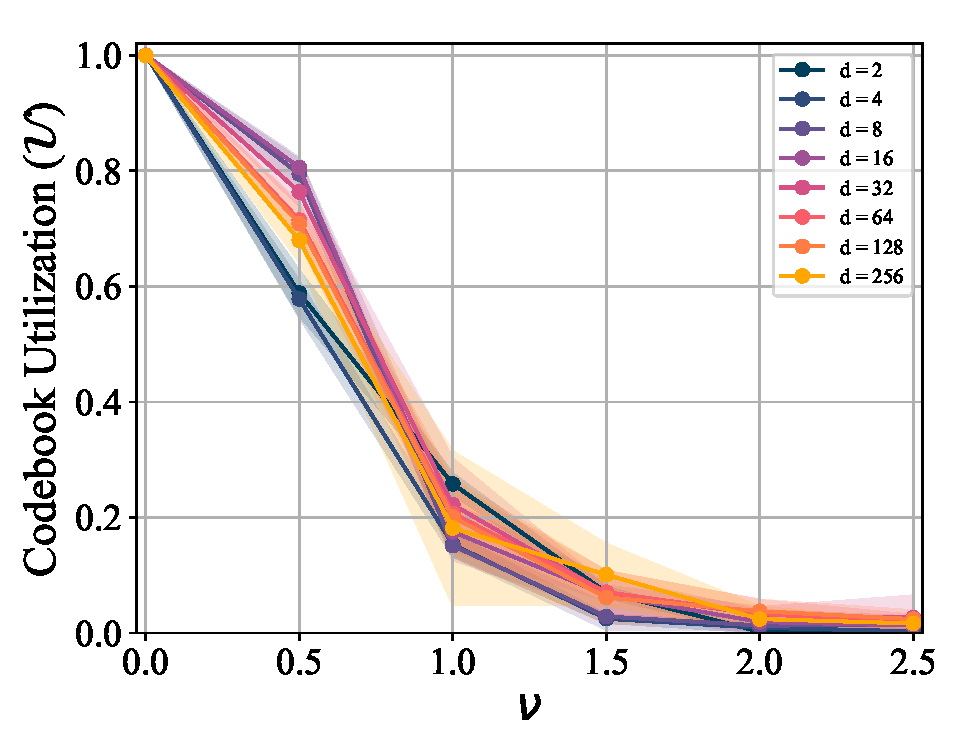
\includegraphics[width=0.16\textwidth]{figs/quantitative_analyses/uniform_distribution/Uniform_FeatureDim_mean_Utili.pdf}
	}
	\hspace{-0.39cm}
	\subfloat[$\cU$ {w.r.t.} $N$]{\label{fig:uniform_featuresize_mean_utilization}
		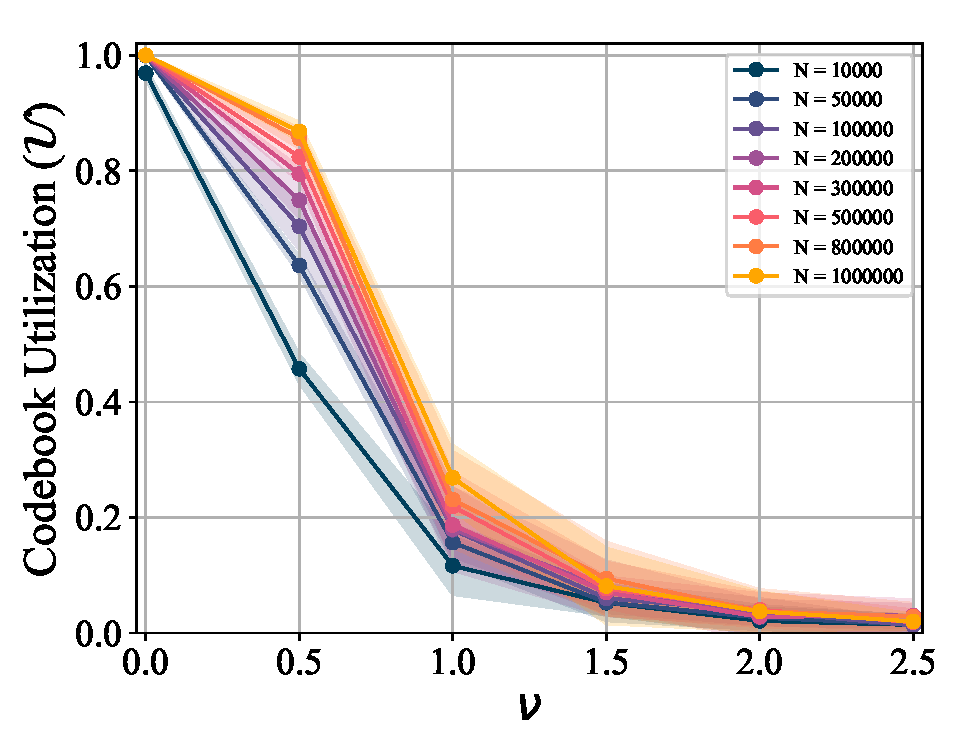
\includegraphics[width=0.16\textwidth]{figs/quantitative_analyses/uniform_distribution/Uniform_FeatureSize_mean_Utili.pdf}
	}
    \hspace{-0.39cm}
	\subfloat[$\cU$ {w.r.t.} $K$]{ \label{fig:uniform_codebooksize_sigma_utilization}  
		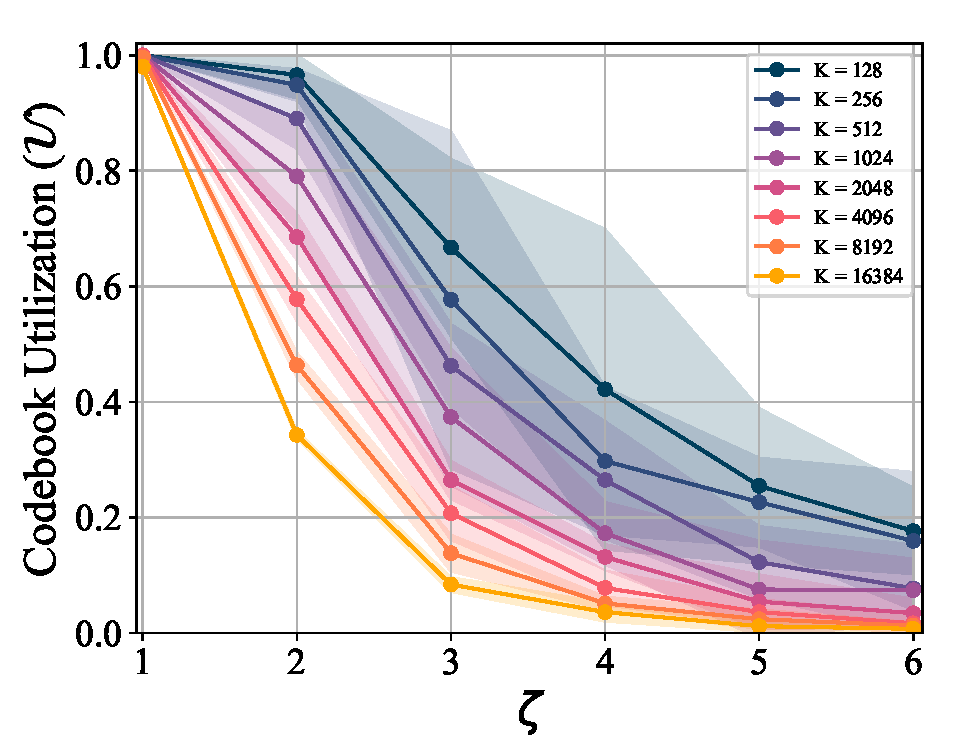
\includegraphics[width=0.16\textwidth]{figs/quantitative_analyses/uniform_distribution/Uniform_CodebookSize_Var_Util.pdf}
	}
    \hspace{-0.39cm}
	\subfloat[$\cU$ {w.r.t.} $d$]{\label{fig:uniform_featuredim_sigma_utilization}
		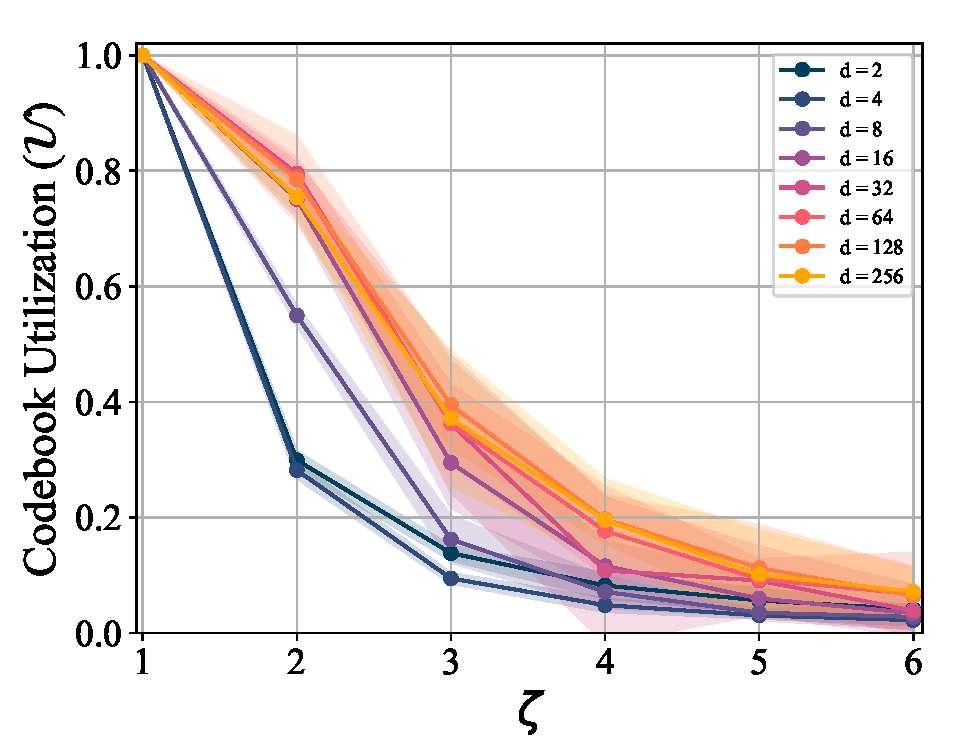
\includegraphics[width=0.16\textwidth]{figs/quantitative_analyses/uniform_distribution/Uniform_FeatureDim_Var_Util.pdf}
	}
    \hspace{-0.39cm}
	\subfloat[$\cU$ {w.r.t.} $N$]{\label{fig:uniform_featuresize_sigma_utilization}
		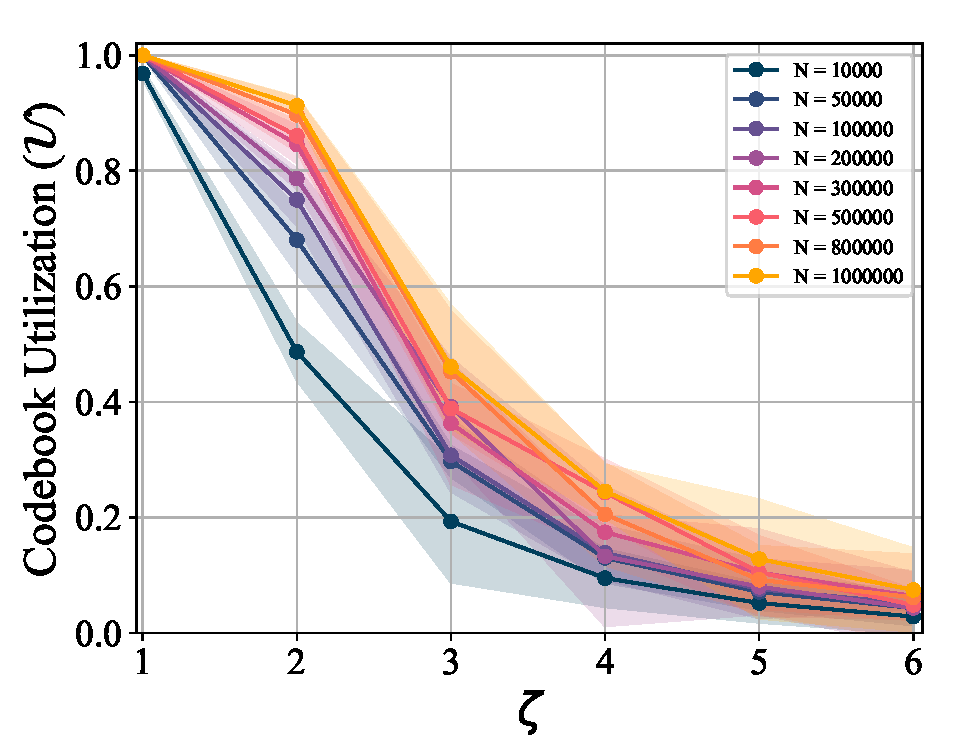
\includegraphics[width=0.16\textwidth]{figs/quantitative_analyses/uniform_distribution/Uniform_FeatureSize_Var_Util.pdf}
	}
    %\vspace{-5pt}
    %%%%%%%%%%%%%%%%%%%%%%%%%%Codebook Perplexity%%%%%%%%%%%%%%%%%%%%%%%%%
    \hspace{-0.8cm}
	\subfloat[$\mathcal{C}$ {w.r.t.} $K$]{ \label{fig:uniform_codebooksize_mean_perplexity}  
		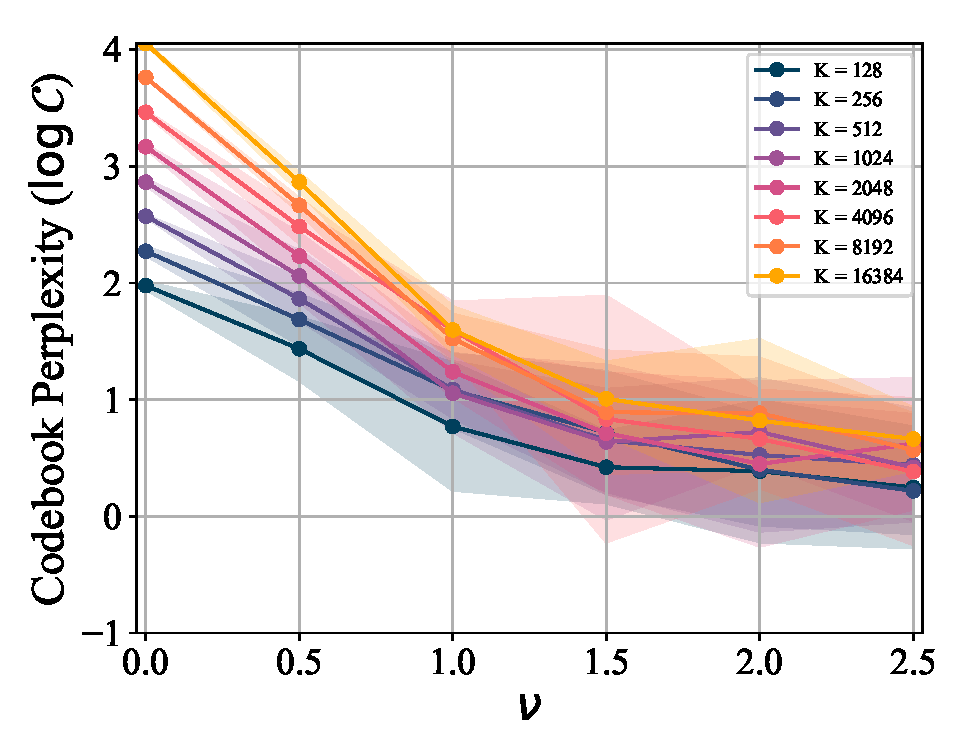
\includegraphics[width=0.16\textwidth]{figs/quantitative_analyses/uniform_distribution/Uniform_CodebookSize_mean_ppl.pdf}
        }
	\hspace{-0.39cm}
	\subfloat[$\mathcal{C}$ {w.r.t.} $d$]{\label{fig:uniform_featuredim_mean_perplexity}
		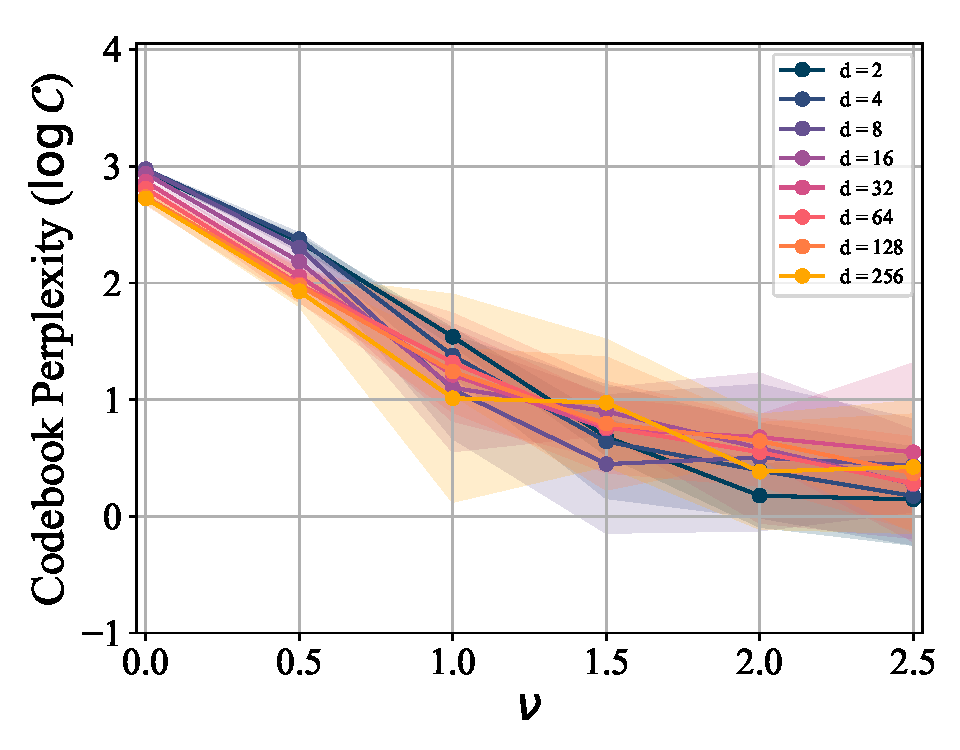
\includegraphics[width=0.16\textwidth]{figs/quantitative_analyses/uniform_distribution/Uniform_FeatureDim_mean_ppl.pdf}
	}
	\hspace{-0.39cm}
	\subfloat[$\mathcal{C}$ {w.r.t.} $N$]{\label{fig:uniform_featuresize_mean_perplexity}
		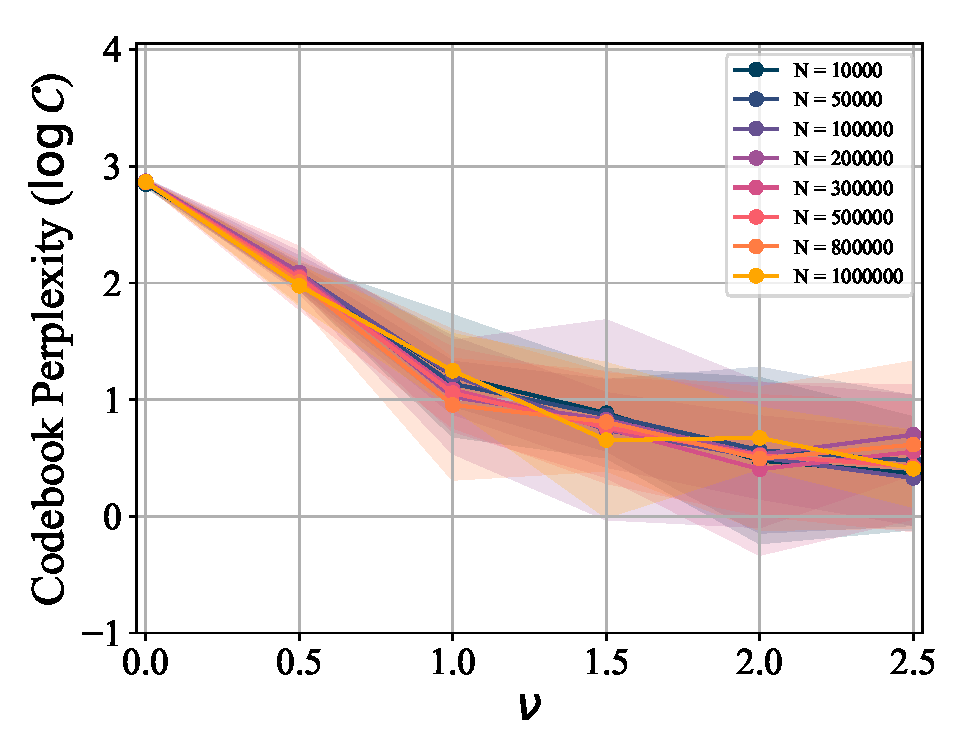
\includegraphics[width=0.16\textwidth]{figs/quantitative_analyses/uniform_distribution/Uniform_FeatureSize_mean_ppl.pdf}
	}
    \hspace{-0.39cm}
	\subfloat[$\mathcal{C}$ {w.r.t.} $K$]{ \label{fig:uniform_codebooksize_sigma_perplexity}  
		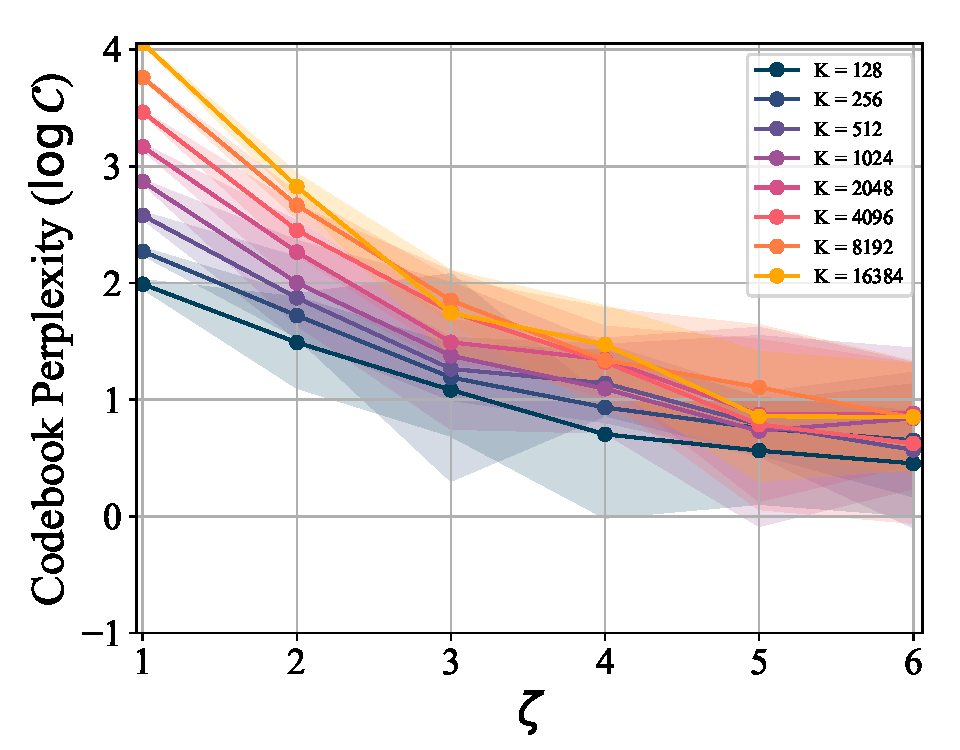
\includegraphics[width=0.16\textwidth]{figs/quantitative_analyses/uniform_distribution/Uniform_CodebookSize_Var_ppl.pdf}
	}
    \hspace{-0.39cm}
	\subfloat[$\mathcal{C}$ {w.r.t.} $d$]{\label{fig:uniform_featuredim_sigma_perplexity}
		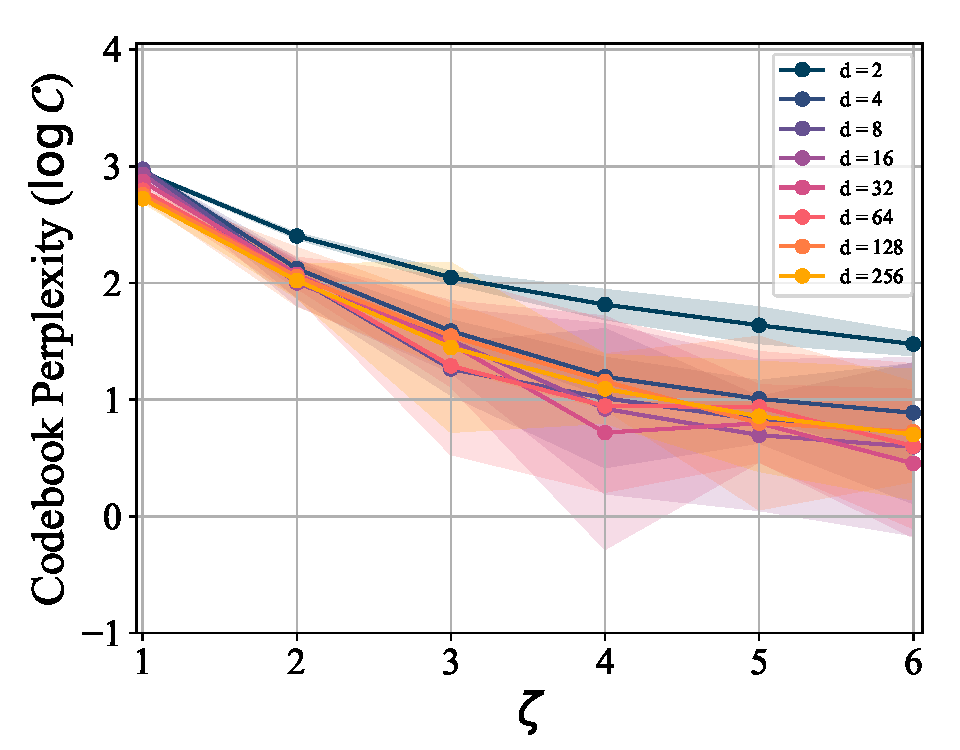
\includegraphics[width=0.16\textwidth]{figs/quantitative_analyses/uniform_distribution/Uniform_FeatureDim_Var_ppl.pdf}
	}
    \hspace{-0.39cm}
	\subfloat[$\mathcal{C}$ {w.r.t.} $N$]{\label{fig:uniform_featuresize_sigma_perplexity}
		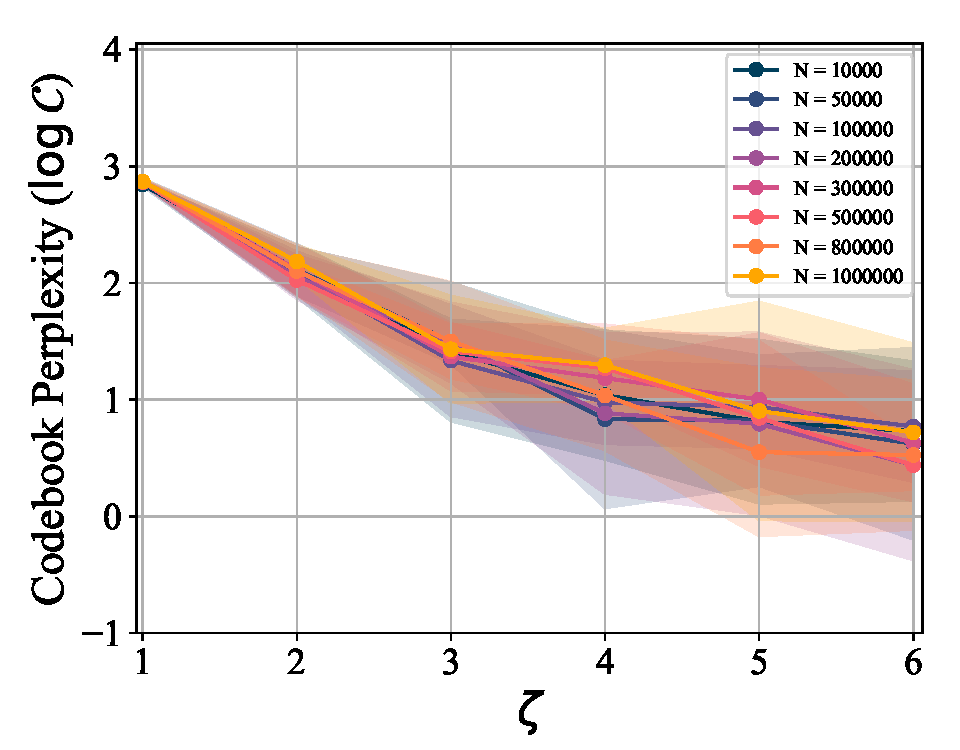
\includegraphics[width=0.16\textwidth]{figs/quantitative_analyses/uniform_distribution/Uniform_FeatureSize_Var_ppl.pdf}
	}
    \vspace{-1ex}
	\caption{Quantitative analyses of the criterion triple when $\mathcal{P}_A$ and $\mathcal{P}_B$ are uniform distributions.}
    \vspace{-2ex}
	\label{fig:quantitative analysis uniform distribution}
\end{figure*}
\fi

We begin by assuming that the distributions $\mathcal{P}_A$ and $\mathcal{P}_B$ are Gaussian. We generate a set of feature vectors $\{\bz_i\}_{i=1}^N$ from $\mathcal{N}_d(\bm 0,  \bm I)$ and a set of code vectors $\{\be_k\}_{k=1}^K$ from $\mathcal{N}_d(\mu \cdot \m 1, \bm I)$, with $\mu$ varying within $\{0.0, 0.5, 1.0, 1.5, 2.0, 2.5\}$. The criterion triple results are presented in Figures~\ref{fig:gaussian_codebooksize_mean_error} to~\ref{fig:gaussian_featuresize_mean_error}, Figures~\ref{fig:gaussian_codebooksize_mean_utilization} to~\ref{fig:gaussian_featuresize_mean_utilization}, and Figures~\ref{fig:gaussian_codebooksize_mean_perplexity} to~\ref{fig:gaussian_featuresize_mean_perplexity}. Across all tested configurations of $K, d, N$, we consistently observe that when $\mu = 0$ — indicating identical distributions between $\mathcal{P}_A$ and $\mathcal{P}_B$ — the criterion triple achieves the lowest $\cE$, highest $\cU$, and largest $\mathcal{C}$. This empirical evidence reinforces the effectiveness of aligning feature and codebook distributions in VQ.

Additionally, we further analyze the criterion triple by varying the covariance matrix. We sample a set of feature vectors $\{\bz_i\}_{i=1}^N$ from the distribution $\mathcal{N}_d(\bm 0, \bm I)$ and a set of code vectors $\{\be_k\}_{k=1}^K$ from $\mathcal{N}_d(\bm 0, \sigma^2 \bm I)$, where $\sigma$  is selected from $\{ 1, 2, 3, 4, 5, 6\}$. The results for the criterion triple are shown in Figures~\ref{fig:gaussian_codebooksize_sigma_error} to~\ref{fig:gaussian_featuresize_sigma_error}, Figures~\ref{fig:gaussian_codebooksize_sigma_utilization} to~\ref{fig:gaussian_featuresize_sigma_utilization}, and Figures~\ref{fig:gaussian_codebooksize_sigma_perplexity} to~\ref{fig:gaussian_featuresize_sigma_perplexity}. When $\sigma = 1$, indicating identical distributions between $\mathcal{P}_A$ and $\mathcal{P}_B$, all three evaluation criteria reach their optimal values: the lowest $\cE$, highest $\cU$, and largest $\mathcal{C}$ across all tested values of $K, d, N$. This result corroborates our earlier findings.

\subsection{Codebook Distribution and Feature Distribution are Unifrom Distributions}
\label{appendix:analyses under uniform distribution}

The above conclusion holds when $\mathcal{P}_A$ and $\mathcal{P}_B$ are other types of distributions, such as the uniform distribution. As shown in Figure~\ref{fig:quantitative analysis uniform distribution}, we sample a set of feature vectors $\{\bz_i\}_{i=1}^N$ from the distribution $\unif_d(-1, 1)$ and a set of code vectors $\{\be_k\}_{k=1}^K$ from $\unif_d(\nu-1, \nu+1)$, where $\nu$ is selected from the set  $\{ {0.0}, {0.5}, {1.0}, {1.5}, {2.0}, {2.5}\}$ or from $\unif_d(-\zeta, \zeta)$, with $\zeta$ drawn from the set $\{ 1, 2, 3, 4, 5, 6\}$. We observe that when $\mu = 0$ or $\zeta = 1$—indicating that $\mathcal{P}_A$  and $\mathcal{P}_B$ have identical distributions—the performance in terms of the criterion triple is optimal, achieving the lowerest $\cE$, the highest $\cU$, and the largest $\mathcal{C}$ across all tested values of $K, d, N$. Therefore, we conclude that our quantitative analyses are distribution-agnostic and can be generalized to other distributions.

\section{Statistical Distances over Gaussian Distributions}
\label{appendix: distribution distance}
We first introduce the definition of Wasserstein distance. 
\begin{definition}
\label{def:wasserstien distance}
The Wasserstein distance or earth-mover distance with $p$ norm is defined as below:
\begin{equation}
W_{p}(\mathbb{P}_r, \mathbb{P}_g) = (\inf_{\gamma \in \Pi(\mathbb{P}_r ,\mathbb{P}_g)} \mathbb{E}_{(x, y) \sim \gamma}\big[\|x - y\|^{p}\big])^{1/p}~.
\label{eq:def wasserstein distance}
\end{equation}
\end{definition} where $\Pi(\mathcal{P}_r,\mathcal{P}_g)$ denotes the set of all joint distributions $\gamma(x,y)$ whose marginals are $\mathcal{P}_r$ and $\mathcal{P}_g$ respectively. Intuitively, when viewing each distribution as a unit amount of earth/soil, the Wasserstein distance (also known as earth-mover distance) represents the minimum cost of transporting ``mass'' from $x$ to $y$ to transform distribution $\mathcal{P}_r$ into distribution $\mathcal{P}_g$. When $p=2$, this is called the quadratic Wasserstein distance.

In this paper, we achieve distributional matching using the quadratic Wasserstein distance under Gaussian distribution assumptions. We also examine other statistical distribution distances as potential loss functions for distributional matching and compare them with the Wasserstein distance. Specifically, we provide the Kullback-Leibler divergence and the Bhattacharyya distance over Gaussian distributions in Lemma~\ref{theorem:kl distance} and Lemma~\ref{theorem:bd distance}. It can be observed that the KL divergence for two Gaussian distributions involves calculating the determinant of covariance matrices, which is computationally expensive in moderate and high dimensions. Moreover, the calculation of the determinant is sensitive to perturbations and it requires full rank (In the case of not full rank, the determinant is zero, rendering the logarithm of zero undefined), which can be impractical in many cases. Other statistical distances like Bhattacharyya Distance suffer from the same issue. In contrast, quadratic Wasserstein distance does not require the calculation of the determinant and full-rank covariance matrices.

\begin{lemma}[Kullback-Leibler divergence~\cite{Lindley1959InformationTA}] \label{theorem:kl distance} 
Suppose two random variables $\m Z_1 \sim \mathcal{N}(\bm \mu_1, \m \Sigma_1)$ and $\m Z_2 \sim \mathcal{N}(\bm \mu_2, \m \Sigma_2)$ obey multivariate normal distributions, then Kullback-Leibler divergence between $\m Z1$ and $\m Z_2$ is:
\begin{align}
\KL(\m Z_1, \m Z_2) = \frac{1}{2}((\bm \mu_1-\bm \mu_2)^T \m \Sigma_2^{-1}(\bm \mu_1-\bm \mu_2) + \tr(\m \Sigma_2^{-1}\m \Sigma_1-\m I) + \ln{\frac{\det{\m \Sigma_2}}{\det \m \Sigma_1}}). \nonumber
\end{align}
\end{lemma}

\begin{lemma}
[Bhattacharyya Distance~\cite{Bhattacharyya1943OnAM}]
\label{theorem:bd distance}
Suppose two random variables $\m Z_1 \sim \mathcal{N}(\bm \mu_1, \m \Sigma_1)$ and $\m Z_2 \sim \mathcal{N}(\bm \mu_2, \m \Sigma_2)$ obey multivariate normal distributions, $\m \Sigma = \frac{1}{2}(\m \Sigma_1 + \m \Sigma_2)$, then bhattacharyya distance between $\m Z1$ and $\m Z_2$ is:
\begin{align}
\mathcal{D}_{\textrm{B}}(\m Z_1, \m Z_2) = \frac{1}{8}(\bm \mu_1-\bm \mu_2)^T \m \Sigma^{-1}(\bm \mu_1-\bm \mu_2) + \frac{1}{2}\ln \frac{\det \m \Sigma}{\sqrt{\det \m \Sigma_1 \det \m \Sigma_2}}. \nonumber
\end{align}
\end{lemma}

\begin{figure}[t]
    \centering
    \vspace{-2ex}
    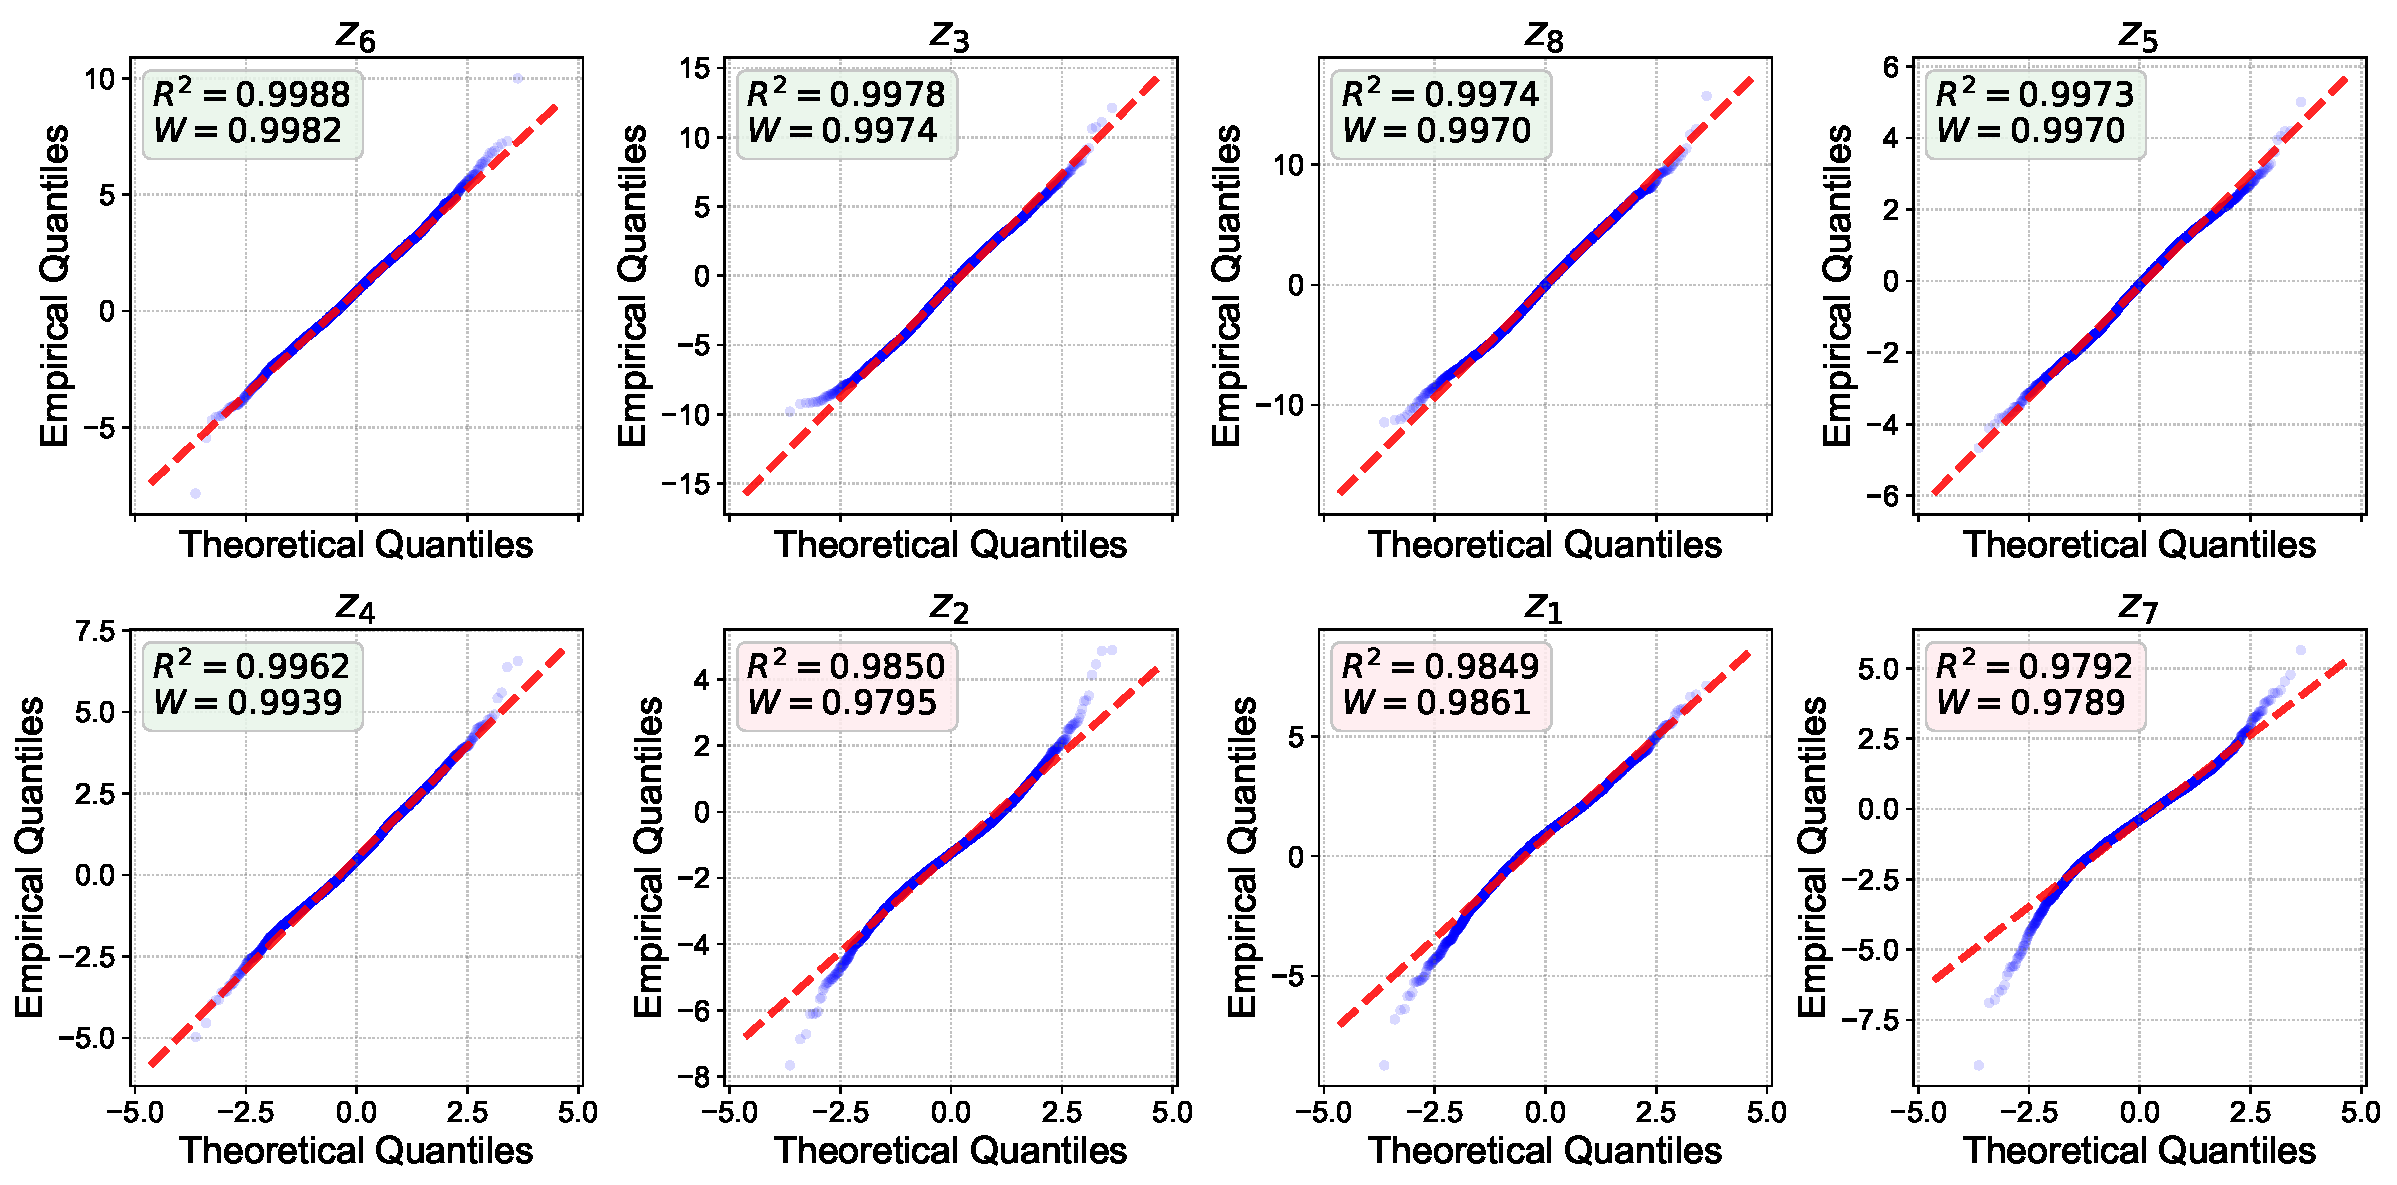
\includegraphics[width=\textwidth]{figs/Gaussion/qq_plots_1d_full.pdf}
    \vspace{-3ex}
    \caption{Comprehensive Q--Q plots for all latent dimensions. Subplots are ordered from the best-fitting dimension $z_6$ (top-left) to the least-fitting dimension $z_7$ (bottom-right) according to the $R^2$ score. \textbf{Visualization:} For visual clarity, blue points show a random subset of 5,000 samples. \textbf{Statistics:} The annotated $R^2$ and Shapiro--Wilk $W$ statistics (green/red boxes) are computed on the \textbf{full validation set ($N=409{,}600$)}. Across all dimensions, the Q--Q plots indicate a strong Gaussian fit for the central mass of the distributions, with only mild deviations in the extreme tails.}
    \label{fig:qq_full}
    \vspace{-2ex}
\end{figure}

\begin{figure}[!t]
    \centering
    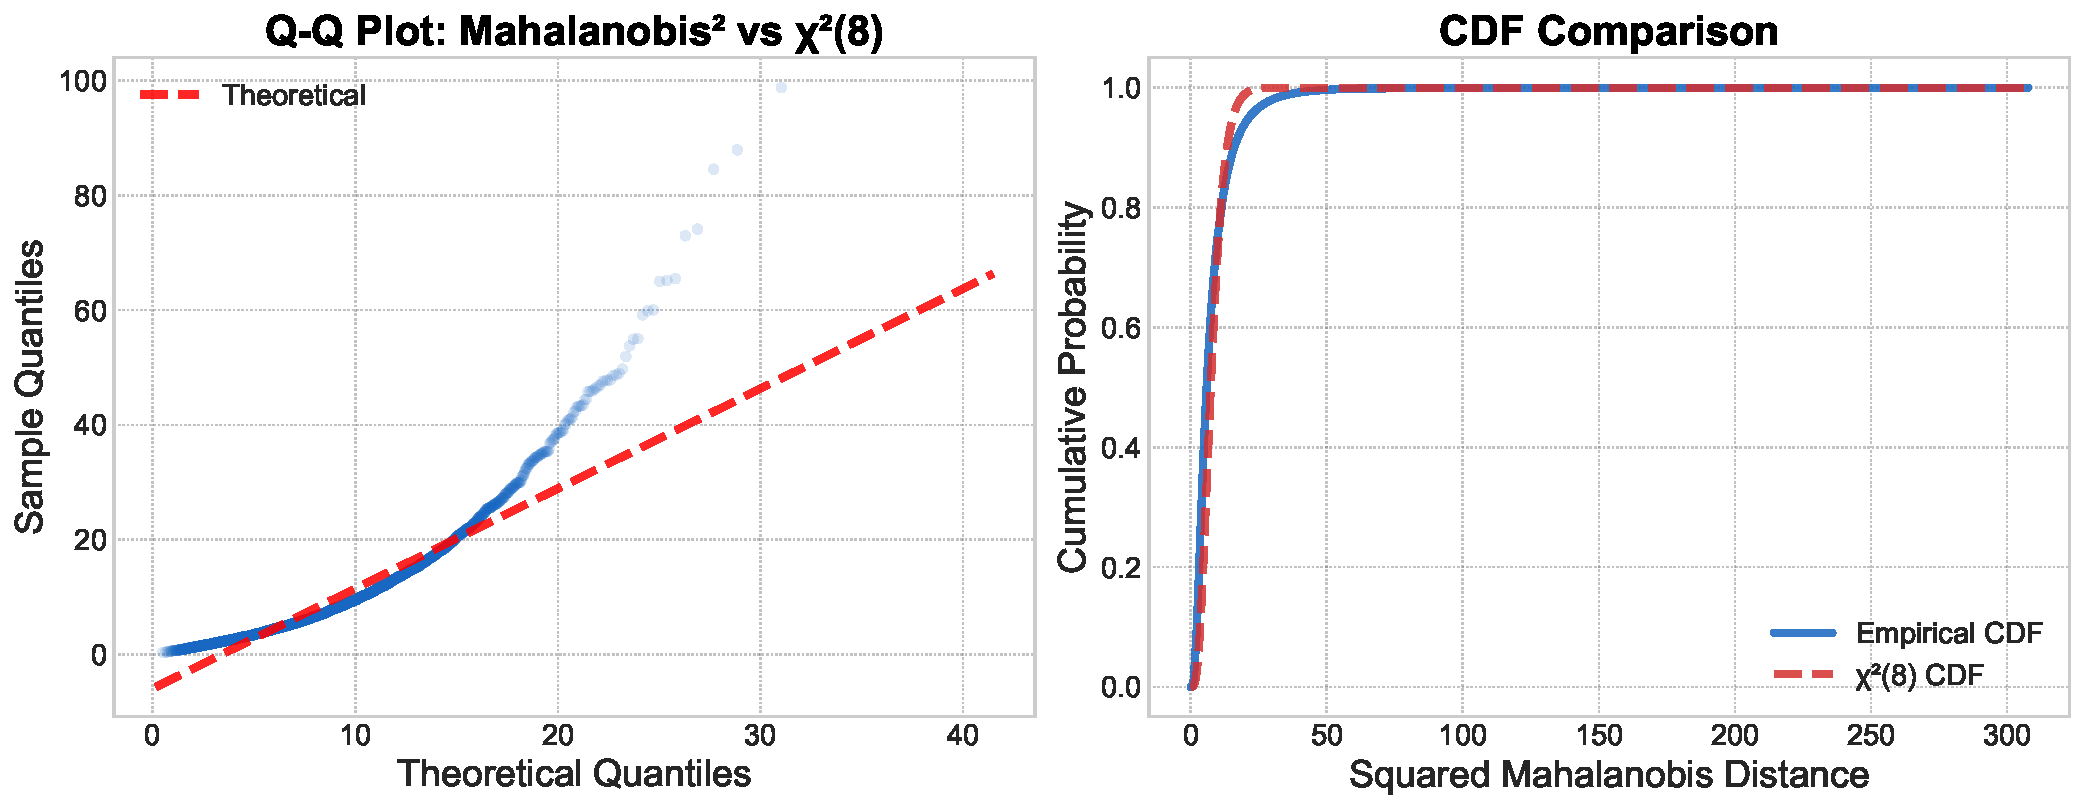
\includegraphics[width=0.95\textwidth]{figs/Gaussion/mahalanobis_8d.pdf}
    \vspace{-1ex}
    \caption{Multivariate normality assessment using Mahalanobis distance. Left (Q--Q plot): The squared Mahalanobis distances of the latent features are compared against the theoretical $\chi^2_8$ quantiles. Deviations are primarily observed in the extreme tails, while the bulk of the samples closely follows the reference line. Right (CDF): The empirical cumulative distribution function (blue solid) closely matches the theoretical $\chi^2_8$ CDF (red dashed) over the primary probability mass, indicating strong agreement in the high-density region.}
    \label{fig:mahalanobis}
    \vspace{-3ex}
\end{figure}

\section{Statistical Assessment of Gaussianity}
\label{sec:normality_tests}
To further validate the Gaussian assumption discussed in Section~\ref{sec:vqvae experiments}, we conduct a comprehensive set of univariate and multivariate normality tests on the validation set. Specifically, we analyze $N=409{,}600$ latent feature vectors ($d=8$), extracted from 1,600 images in the FFHQ dataset.

\textbf{Univariate Analysis.} 
Figure~\ref{fig:qq_full} shows the Q--Q plots for all eight dimensions of the latent feature vector, sorted by their $R^2$ goodness-of-fit scores. Consistent with the observations in the main paper, the majority of dimensions ($z_6, z_3, z_8, z_5, z_4$) demonstrate an excellent fit to the Gaussian distribution, with $R^2 > 0.99$. Although the remaining dimensions exhibit mild deviations in the extreme tails, their Shapiro--Wilk statistics remain high ($W > 0.97$), indicating that the central mass of the distributions is well approximated by a Gaussian.

\textbf{Multivariate Analysis.} 
To assess joint normality, we compute the squared Mahalanobis distance for each validation sample,
\[
d_i^2 = (z_i - \mu)^\top \Sigma^{-1} (z_i - \mu).
\]
Under the multivariate Gaussian hypothesis, $d_i^2$ should follow a Chi-squared distribution with $d=8$ degrees of freedom ($\chi^2_8$). The results are shown in Figure~\ref{fig:mahalanobis}. The Q--Q plot (Left) indicates strong agreement between the empirical and theoretical quantiles for the majority of samples, particularly in the high-density region near the origin, while heavier tails emerge only in the extreme quantiles. To further quantify this alignment, Figure~\ref{fig:mahalanobis} (Right) compares the cumulative distribution functions (CDFs). The empirical CDF (blue solid line) closely matches the theoretical $\chi^2_8$ CDF (red dashed line) across the primary probability mass.

Overall, while deep feature representations naturally exhibit heavy-tailed behavior due to outliers, both univariate and multivariate tests consistently indicate that the bulk of the distribution is well modeled by a Gaussian. This provides strong empirical justification for using the Wasserstein distance, which is derived under Gaussian assumptions, as an efficient and effective optimization surrogate. Moreover, the comparable performance of MMD VQ, which does not impose any parametric distributional assumptions, further suggests that the Gaussian approximation captures the essential statistical structure required for high-fidelity tokenization.

\begin{table*}[!h]
\centering 
\small
\vspace{-1ex}
\caption{Hyperparameters for the experiments in Table~\ref{tab:vqvae ffhq},~\ref{tab:vqvae imagenet},~\ref{tab:reconstruction_IN-main table}, ~\ref{tab:vqvae cifar10},~\ref{tab:vqvae svhn},~\ref{tab:vqgan tranplant ffhq}.}
\label{table:vqvae_hparams}
\vspace{-1ex}
\begin{tabular}{@{}lcccc@{}}
\toprule
Frameworks & VQ-VAE & VQ-VAE & VQGAN  & VQGAN\\
\midrule
\multicolumn{1}{l|}{Dataset} & CIFAR-10/SVHN & FFHQ/ImageNet & FFHQ & ImageNet \\
\multicolumn{1}{l|}{Input size} & $32\times 32\times 3$ & $256\times 256\times 3$ & $256\times 256\times 3$ & $256\times 256\times 3$\\
\multicolumn{1}{l|}{Latent size} & $8\times 8 \times 8$ & $16\times 16 \times 8$ & $16\times 16 \times 32$ & $16\times 16 \times 32$ \\
\multicolumn{1}{l|}{encoder/decoder channels} & $64$ & $64$ & $160$ & $160$\\
\multicolumn{1}{l|}{encoder/decoder channel mult.} & $[1, 1, 2]$ & $[1, 1, 2, 2, 4]$ & $[1, 1, 2, 2, 4]$ & $[1, 1, 2, 2, 4]$ \\
\multicolumn{1}{l|}{Batch size} & 128 & 32 & 32 & 32\\
\multicolumn{1}{l|}{Initial Learning rate $lr$} & $5\times 10^{-5}$ & $5\times 10^{-5}$ & $1\times 10^{-5}$ & $1\times 10^{-5}$\\
\multicolumn{1}{l|}{Perceptual loss Coefficient} & $0$ & $0$ & $1.0$ & $1.0$\\
\multicolumn{1}{l|}{Adversarial loss Coefficient} & $0$ & $0$ & $0.4$ & $0.4$\\
\multicolumn{1}{l|}{Codebook dimensions} & $8$ & $8$ & $32$  & $32$\\
\multicolumn{1}{l|}{Training Epochs} & $50$ & $30/4$ & $30$ & $5/10/15$ \\
\multicolumn{1}{l|}{GPU Resources} & 1 V100 16GB &  1 A100 40GB &  2 H100 80GB & 2 H100 80GB \\
\bottomrule
\end{tabular}
\vspace{-3ex}
\end{table*}

\section{The Experimental Details} 
\label{appendix:synthetic experiment details}

\subsection{Synthetic Experimental Details in Section~\ref{sec:effects of distribution matching} } \label{appendix:details part1}

As depicted in Figure~\ref{fig:criterion triple analysis} in Section~\ref{sec:effects of distribution matching}, we conduct a qualitative analyses of the criterion triple. Specifically, we sample a set of feature vectors $\{\bz_i\}_{i=1}^N$ from within the red circle, and a collection of code vectors $\{\be_k\}_{k=1}^K$ from within the green circle, with parameters set to $K=400$, $N=10000$ and $d=2$ for the calculation of the criterion triple $(\cE, \cU, \mathcal{C})$. For the visualization, we select 10\% of the feature vectors and 90\% of the code vectors for plotting.

\subsection{Synthetic Experimental Details in Appendix~\ref{appendix:supplementary comprehensive quantitative analyses}} \label{appendix:details part3}

As illustrate in Figure~\ref{fig:quantitative analysis gaussian distribution} in Appendix~\ref{appendix:analyses under gaussian distribution}, we undertake comprehensive quantitative analyses centered around the criterion triple $(\cE, \cU, \mathcal{C})$. In these analyses, we assume that $\mathcal{P}_A$ and $\mathcal{P}_B$ are Gaussian distributions, from which we sample a set of feature vectors $\{\bz_i\}_{i=1}^N$ and a collection of code vectors $\{\be_k\}_{k=1}^K$. The default parameters are set to $N=200,000$, $K=1024$, and $d=32$ for all figures unless otherwise specified. For instance, in Figure~\ref{fig:gaussian_codebooksize_mean_error}, $N$ and $d$ are taken at their default values, while the $K$ is varied within the set $\{128, 256, 512, 1024, 2048, 4096, 8192, 16284\}$. Additionally, each synthetic experiment is repeated five times, and the average results are reported, along with the calculation of 95\% confidence intervals. In all figures, mean results are represented by points, while the confidence intervals are shown as shaded areas. Identical parameter settings are employed when $\mathcal{P}_A$ and $\mathcal{P}_B$ are uniform distributions, as illustrated in Figure~\ref{fig:quantitative analysis uniform distribution} in Appendix~\ref{appendix:analyses under uniform distribution}.

\subsection{Synthetic Experimental Details in Appendix~\ref{appendix:Impact of Distribution Variance}} \label{appendix:details part4}
We set $K=8192, d=8, N=100000$ when calculating the criterion triple $(\cE, \cU, \mathcal{C})$ in Appendix~\ref{appendix:Impact of Distribution Variance}. Each synthetic experiment is repeated five times, and the average results are reported in Table~\ref{table:distribution variance}. 

\subsection{Synthetic Experimental Details in Section~\ref{sec:atomic setting}} \label{appendix:details part2}
We provide experimental details of Figure~\ref{fig:analysis on criterion triple (VQ)} in Section~\ref{sec:atomic setting}. In our experimental setup, we evaluate five distinct VQ algorithms using the criterion triple $(\cE, \cU, \mathcal{C})$. All experiments run on a single NVIDIA A100 GPU, with a codebook size $K$ of 16,384 and dimensionality $d$ of 8 across all algorithms. Each algorithm trains for 2,000 steps, with 50,000 feature vectors sampled from the specified Gaussian distribution at each step. For \emph{Wasserstein VQ}, Vanilla VQ, and VQ + MLP, we use the SGD optimizer for training. For VQ EMA and Online Clustering, we use classical clustering algorithms—$k$-means~\cite{Bradley1998RefiningIP} and $k$-means++\cite{Arthur2007kmeansTA}—to update code vectors. 



\subsection{Experimental Details in Section~\ref{sec:experiments}}
\label{appendix:experimental details}



\paragraph{Data Augmentation} For FFHQ and ImageNet-1k datasets, we follow LLama Gen~\cite{Sun2024AutoregressiveMB} and apply iterative box downsampling to resize images to 256×256 resolution. For CIFAR-10 and SVHN, the images are kept at their original resolution.

\paragraph{Encoder-Decoder Architecture In VQ-VAE} For the ImageNet and FFHQ datasets, our proposed Wasserstein VQ and all baseline methods adopt identical encoder-decoder architectures and parameter configurations. Across all baselines in these frameworks, the encoder—a U-Net~\cite{Ronneberger2015UNetCN}—downscales the input image by a factor of 16. For CIFAR-10 and SVHN datasets, the encoder reduces the input resolution by a factor of 4. Detailed hyperparameter configurations are summarized in Table~\ref{table:vqvae_hparams}.

\paragraph{Encoder-Decoder Architecture In VQGAN} To accelerate adversarial training in VQGAN, our proposed Wasserstein VQ-a/b/c and Wasserstein VAR-a/b/c models on the ImageNet dataset, as well as the Wasserstein VQ model on the FFHQ dataset, are built upon the VQ-Transplant framework. Within this framework, we deploy the pretrained VAR tokenizer~\cite{Tian2024VisualAM} for initialization. Consequently, the encoder–decoder architecture is identical to that used in the VAR tokenizer.

\paragraph{Training Details in VQ-VAE} All experiments employ identical training settings: we use the AdamW optimizer~\cite{Loshchilov2017DecoupledWD} with $\beta_1=0.9$ and $\beta_1=0.95$, an initial learning rate $lr$, and apply a half-cycle cosine decay schedule following a linear warm-up phase. For specific details on training epochs and batch sizes, refer to Table~\ref{table:vqvae_hparams}.

\paragraph{Training Details in VQ-GAN} Our proposed Wasserstein VQ and Wasserstein VAR were trained on two NVIDIA H100 GPUs using the AdamW optimizer~\cite{Loshchilov2017DecoupledWD} with $\beta_1=0.9$ and $\beta_1=0.95$.
During VQ module substitution, we used an initial learning rate of $10^{-4}$ with linear decay to 
$10^{-5}$.
For decoder adaptation, the learning rate remained constant at $lr = 10^{-5}$. For specific details on training epochs and batch sizes, refer to Table~\ref{table:vqvae_hparams}. For adversarial training, we follow the VQ-Transplant framework~\cite{Fang2025VQTransplant}, which employs a frozen DINO-S~\cite{Caron2021EmergingPI,Oquab2023DINOv2LR} discriminator with an architecture reminiscent of StyleGAN~\cite{Karras2019AnalyzingAI,karras2019style}. Consistent with VQ-Transplant~\cite{Fang2025VQTransplant}, we further incorporate DiffAug~\cite{Zhao2020DifferentiableAF}, consistency regularization~\cite{Zhang2019ConsistencyRF}, and LeCAM regularization~\cite{Tseng2021RegularizingGA} to stabilize discriminator training.

\paragraph{Loss Weight in VQ-VAE} For all three baselines, $\beta$ is typically set to a value within the range $[0.25, 2]$. In our experiments, $\beta$ is set to a fixed value of $1.0$. For our proposed \emph{Wasserstein VQ} model, we set $\beta$ to a much smaller value,  e.g., $\beta=0.1$. The smaller $\beta$ values enable the Wasserstein distance to dominate the loss function, thereby more effectively narrowing the gap between the distributions.

\paragraph{Loss Weight in VQGAN} For our proposed Wasserstein VQ and Wasserstein VAR models, the perceptual loss weight $\lambda_P$ is fixed at 1. In multi-scale quantization experiments, we set $\lambda_G = 0.5$, whereas in fixed-scale quantization experiments, $\lambda_G = 0.4$. The coefficient $\gamma$ is set to 0.2 for all configurations incorporating the Wasserstein distance (i.e., Wasserstein VQ and Wasserstein VAR).



\section{Supplementary Results and Analyses in VQ-VAE Framework}
\subsection{VQ-VAE Performance on  CIFAR-10 and SVHN datasets}
\label{appendix:vqvae cifar-10 and svhn}
Due to space limitations in the main text, we have relocated the VQ-VAE evaluation on CIFAR-10 and SVHN datasets to the appendix. As demonstrated in Table~\ref{tab:vqvae cifar10}, \ref{tab:vqvae svhn}, our Wasserstein VQ consistently outperforms all baselines across both datasets, achieving superior results on nearly all evaluation metrics regardless of codebook size. Notably, we observe that Wasserstein VQ fails to reach 100\% codebook utilization on SVHN, which may be attributed to the dataset’s limited diversity.

\begin{table*}[!h]
  \centering
  \vspace{-1ex}
  \caption{Comparison of VQ-VAEs trained on CIFAR-10 dataset following~\cite{Oord2017NeuralDR}.}
  \label{tab:vqvae cifar10}
  \vspace{-1ex}
  \resizebox{\textwidth}{!}{
  \begin{tabular}{@{}lccccccc@{}} \hline
    Approaches  & Tokens & Codebook Size & $\mathcal{U}$ ({\color{green!60!black}\bfseries$\pmb{\uparrow}$}) & $\mathcal{C}$ ({\color{green!60!black}\bfseries$\pmb{\uparrow}$}) & PSNR({\color{green!60!black}\bfseries$\pmb{\uparrow}$}) & SSIM({\color{green!60!black}\bfseries$\pmb{\uparrow}$}) & Rec. Loss ({\color{green!60!black}\bfseries$\pmb{\downarrow}$}) \\\hline
    Vanilla VQ & 64 & $8192$ & 2.7\% & 186.9 & 27.15 & 0.83 & 0.0147   \\
    EMA VQ & 64 & $8192$ & 99.7\% & 6416.1 & 29.43 & 0.88 & 0.0095  \\
    Online VQ & 64 & $8192$ & 22.1\% & 995.4 & 28.20 & 0.85 & 0.0123  \\
    \textbf{Wasserstein VQ}  & 64 & $8192$ & \textbf{100.0\%} & \textbf{7781.8}  & \textbf{29.88} & \textbf{0.90} & \textbf{0.0085} \\\hline
    Vanilla VQ & 64 & $16384$ & 1.6\% & 220.3 & 27.36 & 0.84 & 0.0141  \\
    EMA VQ & 64 & $16384$ & 80.8\% & 10557.3 & 29.43 & 0.88 & 0.0093\\
    Online VQ & 64 & $16384$ & 13.4\% & 798.5 & 27.54 & 0.82 & 0.0141 \\
    \textbf{Wasserstein VQ}  & 64 & $16384$ & \textbf{100.0\%} & \textbf{15583.7}  & \textbf{30.19} & \textbf{0.90} & \textbf{0.0080}  \\\hline
    Vanilla VQ & 64 & $32768$ & 0.5\% & 154.8 & 27.10 & 0.83 & 0.0150  \\
    EMA VQ & 64 & $32768$ & 54.4\% & 14427.0 & 29.57 & 0.88 & 0.0091 \\
    Online VQ & 64 & $32768$   & 7.2\% & 1556.0 & 28.84 & 0.87 & 0.0106 \\
    \textbf{Wasserstein VQ} & 64 & $32768$ & \textbf{99.0\%} & \textbf{29845.1}  & \textbf{30.63} & \textbf{0.91} & \textbf{0.0071} \\\hline
  \end{tabular}
  \vspace{-8ex}
}
\end{table*}

\begin{table*}[!t]
  \centering
  \vspace{-1ex}
  \caption{Comparison of VQ-VAEs trained on SVHN dataset following~\cite{Oord2017NeuralDR}.}
  \label{tab:vqvae svhn}
  \vspace{-1ex}
  \resizebox{\textwidth}{!}{%
  \begin{tabular}{@{}lccccccc@{}} \hline
    Approaches & Tokens & Codebook Size & $\mathcal{U}$ ({\color{green!60!black}\bfseries$\pmb{\uparrow}$}) & $\mathcal{C}$ ({\color{green!60!black}\bfseries$\pmb{\uparrow}$}) & PSNR({\color{green!60!black}\bfseries$\pmb{\uparrow}$}) & SSIM({\color{green!60!black}\bfseries$\pmb{\uparrow}$}) & Rec. Loss ({\color{green!60!black}\bfseries$\pmb{\downarrow}$}) \\\hline
    Vanilla VQ  & 64 & $8192$ & 8.1\% & 533.1 & 37.81 & 0.97 & 0.0018 \\
    EMA VQ & 64 & $8192$ & 56.8\% & 3363.0 & 40.38 & \textbf{0.98} & 0.0010 \\
    Online VQ  & 64 & $8192$ & 27.8\% & 1325.1 & 39.04 & 0.97 & 0.0016 \\
    \textbf{Wasserstein VQ}  & 64 & $8192$ & \textbf{88.2\%} & \textbf{6154.5}  & \textbf{41.04} & \textbf{0.98} & \textbf{0.0009} \\\hline
    Vanilla VQ & 64 & $16384$ & 3.4\% & 446.0 & 37.87 & 0.97 & 0.0017 \\
    EMA VQ & 64 & $16384$ & 22.2\% & 2593.8 & 40.19 & \textbf{0.98} & 0.0011 \\
    Online VQ & 64 & $16384$ & 13.5\% & 1090.5 & 39.12 & 0.97 & 0.0014  \\
    \textbf{Wasserstein VQ} & 64 & $16384$ & \textbf{87.5\%} & \textbf{11967.2}  & \textbf{41.49} & \textbf{0.98} & \textbf{0.0008}  \\\hline
    Vanilla VQ & 64 & $32768$ & 1.8\% & 467.5 & 37.87 & 0.97 & 0.0017  \\
    EMA VQ & 64 & $32768$ & 35.8\% & 7662.9 & 40.25 & \textbf{0.98} & 0.0010  \\
    Online VQ & 64 & $32768$ & 7.0\% & 1334.8 & 39.26 & 0.97 & 0.0014 \\
    \textbf{Wasserstein VQ} & 64 & $32768$ & \textbf{88.7\%} & \textbf{24376.3}  & \textbf{41.84} & \textbf{0.98} & \textbf{0.0008}  \\\hline
  \end{tabular}
  \vspace{-4ex}
}
\end{table*}

\begin{table*}[!h]
  \centering
  \vspace{-1ex}
  \caption{Supplementary comparison of VQ-VAEs trained on FFHQ dataset following~\cite{Oord2017NeuralDR} w.r.t codebook size $K$.}
  \label{tab:vqvae ffhq codebook size}
  \vspace{-1ex}
  \resizebox{\textwidth}{!}{%
  \begin{tabular}{@{}lccccccc@{}} \hline
    Approaches & Tokens & Codebook Size & $\mathcal{U}$ ({\color{green!60!black}\bfseries$\pmb{\uparrow}$}) & $\mathcal{C}$ ({\color{green!60!black}\bfseries$\pmb{\uparrow}$}) & PSNR({\color{green!60!black}\bfseries$\pmb{\uparrow}$}) & SSIM({\color{green!60!black}\bfseries$\pmb{\uparrow}$}) & Rec. Loss ({\color{green!60!black}\bfseries$\pmb{\downarrow}$})\\\hline
    Vanilla VQ & 256 & 1024 & 51.7\% & 446.2 & 27.64 & 73.0 & 0.0125 \\
    EMA VQ & 256 & 1024 & 74.1\% & 618.9 & 27.66 & 72.7 & 0.0125  \\
    Online VQ & 256 & 1024 & \textbf{100.0\%} & 759.3 & 28.08 & 74.0 & 0.0114  \\
    \textbf{Wasserstein VQ} & 256 & 1024 & \textbf{100.0\%} & \textbf{977.4} & \textbf{28.11} & \textbf{74.4} & \textbf{0.0112} \\\hline
    Vanilla VQ & 256 & 2048 & 27.6\% & 453.0 & 27.78 & 73.8 & 0.0121 \\
    EMA VQ & 256 & 2048 & \textbf{100\%} & 1608.0 & \textbf{28.39} & 74.9 & \textbf{0.0107}  \\
    Online VQ & 256 & 2048 & \textbf{100\%} & 1462.6 & 28.34 & 74.6 & 0.0108  \\
    \textbf{Wasserstein VQ} & 256 & 2048 & \textbf{100\%} & \textbf{1840.5} & 28.32 & \textbf{75.3} & \textbf{0.0107} \\\hline
    Vanilla VQ & 256 & 4096 & 12.5\% & 435.0 & 27.84 & 73.7 & 0.0119 \\
    EMA VQ & 256 & 4096 & 76.7\% & 2443.1 & 28.49 & 75.0 & 0.0104 \\
    Online VQ & 256 & 4096 & 70.7\% & 1600.0 & 28.25 & 74.1 & 0.0110 \\
    \textbf{Wasserstein VQ} & 256 & 4096 & \textbf{100\%} & \textbf{3895.4} & \textbf{28.54} & \textbf{75.1} & \textbf{0.0102} \\\hline
    Vanilla VQ  & 256 & 8192 & 5.6\% & 398.1 & 27.69 & 73.5 & 0.0122  \\
    EMA VQ & 256 & 8192 & 28.9\% & 1839.2 & 28.39 & 74.8 & 0.0106  \\
    Online VQ & 256 & 8192 & 34.9\% & 1474.4 & 28.15 & 73.9 & 0.0113 \\
    \textbf{Wasserstein VQ} & 256 & 8192 & \textbf{100\%} & \textbf{7731.5} & \textbf{28.81} & \textbf{76.2} & \textbf{0.0099} \\\hline
  \end{tabular}
  \vspace{-8ex}
}
\end{table*}

\begin{table*}[!t]
  \centering
  \vspace{-1ex}
  \caption{Analysis On codebook dimension by the comparison of VQ-VAEs trained on CIFAR-10 dataset following~\cite{Oord2017NeuralDR}. (The codebook size $K$ is fixed to 16384)}
  \label{tab:vqvae cifar-10 codebook dimension}
  \vspace{-1ex}
  \resizebox{\textwidth}{!}{%
  \begin{tabular}{@{}lccccccc@{}} \hline
    Approaches  & Tokens & Codebook Dim & $\mathcal{U}$ ({\color{green!60!black}\bfseries$\pmb{\uparrow}$}) & $\mathcal{C}$ ({\color{green!60!black}\bfseries$\pmb{\uparrow}$}) & PSNR({\color{green!60!black}\bfseries$\pmb{\uparrow}$}) & SSIM({\color{green!60!black}\bfseries$\pmb{\uparrow}$}) & Rec. Loss ({\color{green!60!black}\bfseries$\pmb{\downarrow}$})\\\hline
    Vanilla VQ & 256 & 2 & 3.8\% & 532.2 & 27.00 & 0.80 & 0.0162 \\
    EMA VQ & 256 & 2 & 97.6\% & \textbf{14460.3} & 27.25 & 0.80 & \textbf{0.0155} \\
    Online VQ & 256 & 2 & 9.0\% & 611.8 & 26.62 & 0.79 & 0.0178 \\
    \textbf{Wasserstein VQ} & 256 & 2 & \textbf{99.3\%} & 12278.9  & \textbf{27.30} & \textbf{0.81} & \textbf{0.0155} \\\hline
    Vanilla VQ  & 256 & 4 & 1.3\% & 176.7 & 27.15 & 0.83 & 0.0149 \\
    EMA VQ  & 256 & 4 & 99.8\% & 13153.9 & 29.57 & 0.89 & 0.0092 \\
    Online VQ  & 256 & 4 & 11.1\% & 877.7 & 26.69 & 0.79 & 0.0173 \\
    \textbf{Wasserstein VQ}  & 256 & 4 & \textbf{100.0\%} & \textbf{15724.7}  & \textbf{29.93} & \textbf{0.89} & \textbf{0.0087} \\\hline
    Vanilla VQ   & 256 & 8 & 1.6\% & 220.3 & 27.36 & 0.84 & 0.0141 \\
    EMA VQ  & 256 & 8 & 80.8\% & 10557.3 & 29.43 & 0.88 & \textbf{0.0009} \\
    Online VQ & 256 & 8  & 13.4\% & 798.5 & 27.54 & 0.82 & 0.0141 \\
    \textbf{Wasserstein VQ} & 256 & 8  & \textbf{100.0\%} & \textbf{15583.7}  & \textbf{30.19} & \textbf{0.90} & 0.0080 \\\hline
    Vanilla VQ & 256 & 16  & 1.1\% & 150.8 & 27.05 & 0.83 & 0.0152 \\
    EMA VQ & 256 & 16 & 32.5\% & 4169.2 & 29.31 & 0.88 & 0.0099 \\
    Online VQ & 256 & 16 & 18.2\% & 2051.0 & 28.29 & 0.85 & 0.0122 \\
    \textbf{Wasserstein VQ} & 256 & 16 & \textbf{99.2\%} & \textbf{14832.2}&\textbf{30.27}  & \textbf{0.91} & \textbf{0.0078} \\\hline
    Vanilla VQ & 256 & 32 & 0.7\% & 94.37 & 26.67 & 0.81 & 0.0165 \\
    EMA VQ & 256 & 32 & 7.0\% & 942.7 & 28.24 & 0.85 & 0.0122 \\
    Online VQ & 256 & 32 & 18.8\% & 2278.0 & 28.92 & 0.87 & 0.0104 \\
    \textbf{Wasserstein VQ} & 256 & 32 & \textbf{96.4\%} & \textbf{14056.9}  & \textbf{30.39} & \textbf{0.91} & \textbf{0.0076} \\\hline
    \vspace{-6ex}
  \end{tabular}
}
\end{table*}

\begin{table*}[!t]
  \centering
  \vspace{-1ex}
  \caption{Sensitivity analysis of $\gamma$ trained on FFHQ dataset following~\cite{Oord2017NeuralDR}.}
  \label{tab:sensitivity analysis}
  \vspace{-1ex}
  \resizebox{\textwidth}{!}{%
  \begin{tabular}{@{}lcccccccc@{}} \hline
    Approaches &$\gamma$& Tokens & Codebook Size & $\mathcal{U}$ ({\color{green!60!black}\bfseries$\pmb{\uparrow}$}) & $\mathcal{C}$ ({\color{green!60!black}\bfseries$\pmb{\uparrow}$}) & PSNR({\color{green!60!black}\bfseries$\pmb{\uparrow}$}) & SSIM({\color{green!60!black}\bfseries$\pmb{\uparrow}$}) & Rec. Loss ({\color{green!60!black}\bfseries$\pmb{\downarrow}$}) \\\hline
    \textbf{Wasserstein VQ} & 0.0 & 256 & $16384$ & 3.8\% & 527.2 & 27.83 & 73.8 & 0.0119 \\
    \textbf{Wasserstein VQ} & 0.00001 & 256 & $16384$ & 24.8\% & 903.0 & 27.97 & 74.2 &  0.0114\\
    \textbf{Wasserstein VQ} & 0.0001 & 256 & $16384$ & 52.3\% & 6764.3 & 28.70 & 75.5 &  0.0100\\ 
    \textbf{Wasserstein VQ} & 0.001 & 256 & $16384$ & 90.6\% & 9988.0 & 28.93 & 76.7 &  0.0094\\ 
    \textbf{Wasserstein VQ} & 0.01 & 256 & $16384$ & \textbf{100\%} & 14952.5 & 29.06 & 76.7 &  \textbf{0.0092}\\ 
    \textbf{Wasserstein VQ} & 0.1 & 256 & $16384$ & \textbf{100\%} & \textbf{15943.5} & \textbf{29.07} & 76.7 & \textbf{0.0092} \\ 
    \textbf{Wasserstein VQ} & 0.5 & 256 & $16384$ &  \textbf{100\%} & 15713.3 & 29.03 & 76.6 & 0.0093 \\
    \textbf{Wasserstein VQ} & 1.0 & 256 & $16384$ &  \textbf{100\%}& 14712.4 & 29.02 & \textbf{76.9} & 0.0093 \\\hline
  \end{tabular}
  \vspace{-10ex}
}
\end{table*}


\subsection{Analyses on Codebook Size and Dimensionality}
\label{appendix:ablation study}

\paragraph{Analyses of Codebook Size} We investigate the impact of the codebook size $K$  on the performance of VQ by varying across a wide range: $K \in [1024, 2048, 4096, 8192, 16384, 50000, 100000]$. As shown in Table~\ref{tab:vqvae ffhq},~\ref{tab:vqvae ffhq codebook size}, the vanilla VQ model suffers from severe codebook collapse even with a relatively small $K$, such as $K=1024$. In contrast, improved algorithms like EMA VQ and Online VQ can handle smaller codebook sizes effectively, but they still experience codebook collapse when $K$ is very large, e.g., $K\geq 50000$.
Notably, the \emph{Wasserstein VQ} model consistently maintains 100\% codebook utilization, irrespective of the codebook size. This underscores the effectiveness of distributional matching via the quadratic Wasserstein distance in mitigating the issue of codebook collapse.

\paragraph{Analyses of Codebook Dimensionality} We further investigate the impact of codebook dimensionality $d$ on VQ performance. Conducting experiments on CIFAR-10 with dimensionality $d$ ranging from 2 to 32, our proposed Wasserstein VQ consistently outperforms all baselines regardless of dimensionality, as shown in Table~\ref{tab:vqvae cifar-10 codebook dimension}. Notably, we observe the curse of dimensionality phenomenon—performance degrades as dimensionality increases. Vanilla VQ exhibits the most severe degradation, followed by EMA VQ and Online VQ, while our Wasserstein VQ shows only minimal codebook utilization reduction.




\subsection{Sensitivity Analysis on $\gamma$.}
\label{appendix:sensitivity analysis}
We conduct a sensitivity analysis with respect to $\gamma$ on the FFHQ dataset by varying $\gamma \in \{0, 10^{-5}, 10^{-4}, 10^{-3}, 10^{-2}, 10^{-1}, 1\}$. As reported in Table~\ref{tab:sensitivity analysis}, when $\gamma = 0$, Wasserstein VQ yields the worst performance, as it degenerates into the vanilla VQ formulation without distributional matching. As $\gamma$ increases from $10^{-5}$ to $10^{-3}$, the performance of Wasserstein VQ consistently improves. When $\gamma$ reaches $10^{-2}$, Wasserstein VQ achieves full ($100\%$) codebook utilization along with competitive quantitative results. Moreover, within the range $\gamma \in [10^{-2}, 1]$, the performance of Wasserstein VQ remains stable, indicating that the method is not sensitive to the precise choice of $\gamma$ once it exceeds a moderate threshold.


\subsection{Computational Overhead Comparison among Various VQ Approaches}
\label{appendix:computational overhead}
To evaluate the runtime efficiency of different VQ approaches, we measure the forward and backward pass times of the VQ module over 100 iterations across three different codebook sizes, with the feature dimension set to $d=8$ and the number of data samples $N=8192$. As shown in Table~\ref{tab:computational overhead}, even at large codebook sizes (specifically, $K \geq 50,000$), the runtime of Wasserstein VQ is only slightly longer than that of Vanilla VQ. This demonstrates that Wasserstein VQ maintains high computational efficiency, and incorporating the quadratic Wasserstein distance does not introduce significant time overhead. Notably, while Online VQ exhibits substantial runtime increases at large codebook sizes, Wasserstein VQ remains considerably more efficient, further underscoring its scalability.

\subsection{Discussion with VQ-WAE~\cite{Vuong2023VectorQW}}
\label{appendix:VQ-WAE}
VQ-WAE~\cite{Vuong2023VectorQW} introduces an alternative approach to distributional matching by employing Optimal Transport to optimize codebook vectors. Compared with our proposed distributional matching method, there are three key differences.

\textbf{First, regarding theoretical contributions}: VQ-WAE~\cite{Vuong2023VectorQW} claims that achieving optimal transport (OT) between code vectors and feature vectors yields the best reconstruction performance. Their notion of optimality encompasses both the VQ process and the encoder-decoder reconstruction pipeline. While we contend that incorporating complex encoder-decoder functions renders rigorous theoretical analysis intractable, VQ-WAE nevertheless asserts this conclusion. In contrast, our work deliberately excludes encoder-decoder components, focusing solely on the VQ process, which admits rigorous mathematical modeling. Through our proposed criterion triple, we theoretically prove that distributional matching guarantees optimal performance.

\textbf{Second, regarding distribution modeling}: VQ-WAE~\cite{Vuong2023VectorQW} assumes both code vectors and feature vectors follow uniform discrete distributions, whereas our method models them as continuous distributions. Specifically, VQ-WAE~\cite{Vuong2023VectorQW} represents the distributions of feature vectors $\{\bz_i\}_{i=1}^N$ and code vectors $\{\be_k\}_{k=1}^K$ as empirical measures:
\begin{align}
\label{eq:vqwae distribution}
\mathcal{P}_A = \frac{1}{N}\sum_{i=1}^{N} \delta_{\bz_i}, \quad \mathcal{P}_B = \frac{1}{N}\sum_{k=1}^{K} \delta_{\be_k}
\end{align} 
where $\delta_{\bz_i}$ and $\delta_{\be_k}$ denote Dirac delta functions centered at $\bz_i$ and $\be_k$, respectively. To align  $\mathcal{P}_A$ and $\mathcal{P}_B$, VQ-WAE formulates the OT problem as:
\begin{equation}
\label{eq:ot_problem}
\begin{aligned}
&\min_{\mathbf{P} \in \Pi(\mathcal{P}_A, \mathcal{P}_B)} \sum_{i=1}^N \sum_{k=1}^K P_{ik} \|\bz_i - \be_k\|^2, \\
&\text{s.t.} \quad \mathbf{P} \mathbf{1}_K = \frac{1}{N}\mathbf{1}_N, \quad \mathbf{P}^\top \mathbf{1}_N = \frac{1}{K}\mathbf{1}_K, \quad P_{ik} \geq 0 \quad \forall i,k,
\end{aligned}
\end{equation}
where $\mathbf{P}$ is the transport plan, and the feasible set is:
\begin{equation}
\label{eq:coupling_set}
\Pi(\mathcal{P}_A, \mathcal{P}_B) = 
\left\{ 
\mathbf{P} \in \mathbb{R}_+^{N \times K} 
\; \middle| \;
\mathbf{P} \mathbf{1}_K = \frac{1}{N} \mathbf{1}_N, \ 
\mathbf{P}^\top \mathbf{1}_N = \frac{1}{K} \mathbf{1}_K 
\right\}
\end{equation}
In contrast, we simplify the distributional assumption by modeling $\mathcal{P}_A$ and  $\mathcal{P}_B$ as Gaussian distributions.


\begin{table*}[!t]
\centering
\caption{Reconstruction performance ($\downarrow:$ the lower the better and $\uparrow:$ the higher the better). $^{\dagger}$:Results cited from VQ-WAE~\cite{Vuong2023VectorQW}. Codebook size $K$ is fixed to $512$.}
\vspace{-2ex}
\resizebox{0.98\textwidth}{!}{
\begin{tabular}{@{}lrcrrrrrr@{}}
\toprule 
Dataset & Model & Tokens & SSIM ({\color{green!60!black}\bfseries$\pmb{\uparrow}$}) & PSNR ({\color{green!60!black}\bfseries$\pmb{\uparrow}$}) & LPIPS ({\color{green!60!black}\bfseries$\pmb{\downarrow}$}) & Rec. Loss ({\color{green!60!black}\bfseries$\pmb{\downarrow}$})  & Perplexity ({\color{green!60!black}\bfseries$\pmb{\uparrow}$})
\tabularnewline 
\midrule 
CIFAR10 & VQ-VAE$^{\dagger}$  & 64 & 70 & 23.14 & 0.35 & & 69.8  \tabularnewline
 & SQ-VAE$^{\dagger}$  & 64 & 80 & 26.11 & 0.23 & & 434.8 \tabularnewline
 & VQ-WAE$^{\dagger}$  & 64 & 80 & 25.93 & 0.23 & & 497.3 \tabularnewline
 & VQ-WAE (Our run) & 64 & 13 & 14.60 & 0.41 & 0.247 & 1.0 \tabularnewline
 & Vanilla VQ & 64 & 83 & 27.19 & 0.03 & 0.015 &192.5\tabularnewline
 & EMA VQ  & 64 & 84 & 27.97 & 0.04 & 0.013 & 436.1 \tabularnewline
 & Online VQ & 64 & 84 & 27.87 & 0.04  & 0.013 &451.4\tabularnewline
 & \textbf{Wasserstein VQ} & 64 & 86 & 28.26 & 0.03  & 0.012 & 481.7 \tabularnewline
\midrule         
SVHN & VQ-VAE$^{\dagger}$ & 64 & 88 & 26.94 & 0.17  & & 114.6 \tabularnewline
 & SQ-VAE$^{\dagger}$  & 64 & 96 & 35.37 & 0.06 & & 389.8 \tabularnewline
 & VQ-WAE$^{\dagger}$  & 64 & 96 & 34.62 & 0.07 &  & 485.1 \tabularnewline
 & VQ-WAE (Our run) & 64 & 25 & 15.87 & 0.26 & 0.2026 &1.0\tabularnewline
 & Vanilla VQ & 64 & 97 & 38.18 & 0.01 & 0.0016 & 407.1\tabularnewline
 & EMA VQ & 64 & 97 & 38.35 & 0.01 & 0.0017 & 408.9 \tabularnewline
 & Online VQ & 64 & 97 & 38.54 & 0.01 & 0.0017 & 421.5\tabularnewline
 & \textbf{Wasserstein VQ} & 64 & 97& 38.25 & 0.01 & 0.0016 & 423.5 \tabularnewline
\midrule 
\end{tabular}}
\label{tab:vq-wae}
\vspace{-4ex}
\end{table*}

\textbf{Third, regarding computational efficiency}, The OT problem in VQ-WAE is prohibitively complex, whereas our quadratic Wasserstein distance incurs minimal overhead. To mitigate complexity, VQ-WAE employs a Kantorovich potential network. However, upon reproducing their code (no official implementation was released; we derived it from their ICLR 2023 supplementary material, \footnote{See \url{https://openreview.net/forum?id=Z8qk2iM5uLI}. We includes the reproduced code and training logs of VQ-WAE in our supplementary materials.}), 
we observed severe non-convergence—the method degenerated to using a single code vector, failing to achieve distributional matching. Notably, VQ-WAE underperformed all other VQ baselines (Table~\ref{tab:vq-wae}).

In comparison, our quadratic Wasserstein distance (Equation~\ref{eq:wasserstein distance}) requires only low-dimensional matrix operations (e.g., $d=8$), achieving superior performance and effective matching (Figure~\ref{fig:feature codebook visualization}).


\iffalse
\section{Supplementary Results and Analyses in VQ-GAN Framework}

\subsection{Supplementary Reconstruction Results on FFHQ Dataset}
\label{appendix:supplement results on ffhq}
Due to space constraints in the main text, we have moved the VQGAN  evaluation on the FFHQ dataset to the appendix. As shown in Table~\ref{tab:vqgan tranplant ffhq}, Wasserstein VQ achieves a record r-FID of 1.21, substantially outperforming all baselines, including RQVAE~\cite{Lee2022AutoregressiveIG}, VQGAN~\cite{Esser2020TamingTF}, VQGAN-FC~\cite{Yu2021VectorquantizedIM}, VQGAN-EMA~\cite{Razavi2019GeneratingDH}, VQ-WAE~\cite{Vuong2023VectorQW}, MQVAE~\cite{Huang2023NotAI}, and VQGAN-LC~\cite{Zhu2024ScalingTC}.

\begin{table*}[!t]
\centering
\caption{{Reconstruction performance on the FFHQ dataset. Results marked with $^{\dagger}$ are cited from VQGAN-LC \cite{Zhu2024ScalingTC}, and those with $^{\ddagger}$ from VQ-Transplant~\cite{Fang2025VQTransplant}.}}
\vspace{-2ex}
\label{tab:vqgan tranplant ffhq}
\resizebox{\textwidth}{!}{%
\begin{tabular}{@{}lcccccccc@{}}
\toprule
VQs & Tokens & Codebook Size $K$ & $\mathcal{E}$({\color{green!60!black}\bfseries$\pmb{\downarrow}$}) & $\mathcal{U}$ ({\color{green!60!black}\bfseries$\pmb{\uparrow}$}) & PSNR({\color{green!60!black}\bfseries$\pmb{\uparrow}$}) & SSIM({\color{green!60!black}\bfseries$\pmb{\uparrow}$}) & LPIPS ({\color{green!60!black}\bfseries$\pmb{\downarrow}$}) & r-FID({\color{green!60!black}\bfseries$\pmb{\downarrow}$}) \\
\midrule
RQVAE$^{\dagger}$ & 256 & 2048 & - & - & 22.9 & 67.0 & 0.13 & 7.04  \\
VQ-WAE$^{\dagger}$ & 256 & 1024 & - & -  & 22.5 & 66.5 & 0.12 & 4.20 \\
MQVAE$^{\dagger}$ & 256 & 1024 & - & 78.2\% & - & - & -  & 4.55 \\
VQGAN$^{\dagger}$ & 256 & 16384 & - & 2.3\% & 24.4 & 63.3 & 0.12 & 5.25  \\
VQGAN-FC$^{\dagger}$ & 256 & 16384  & - & 10.9\% & 24.8 & 64.6 & 0.11 & 4.86  \\
VQGAN-EMA$^{\dagger}$  & 256 & 16384  & - & 68.2\% & 25.4 & 66.1 & 0.10 & 4.79   \\
VQGAN-LC$^{\dagger}$ & 256 & 100000  & - & 99.5\% & 26.1 & 69.4 & 0.08 & 3.81   \\\midrule
\textbf{Wasserstein VQ} & 512 & 16384 & \textbf{0.153} & 99.7\%   &  \textbf{27.25} & \textbf{75.4} & \textbf{0.075} & \textbf{1.81} \\
\textbf{Wasserstein VQ} & 512 & 32768  & \textbf{0.142} & 99.7\%  & 27.33 & \textbf{75.7} & \textbf{0.072} & \textbf{1.21} \\
\bottomrule
\vspace{-1ex}
\end{tabular}
}
\end{table*}

\subsection{Reconstruction Visualization}
\label{appendix:reconstruction visualization}
To further demonstrate the reconstruction performance, in this section we visualize the reconstructed FFHQ and ImageNet images in Figure~\ref{fig:visual reconstruction ffhq} and~\ref{fig:visual reconstruction imagenet}. As shown, the images reconstructed by our proposed method are nearly identical to the original inputs. In particular, on the FFHQ dataset, only very minor differences can be observed in fine details. 

\noindent
\begin{figure*}[!t]
    \centering
    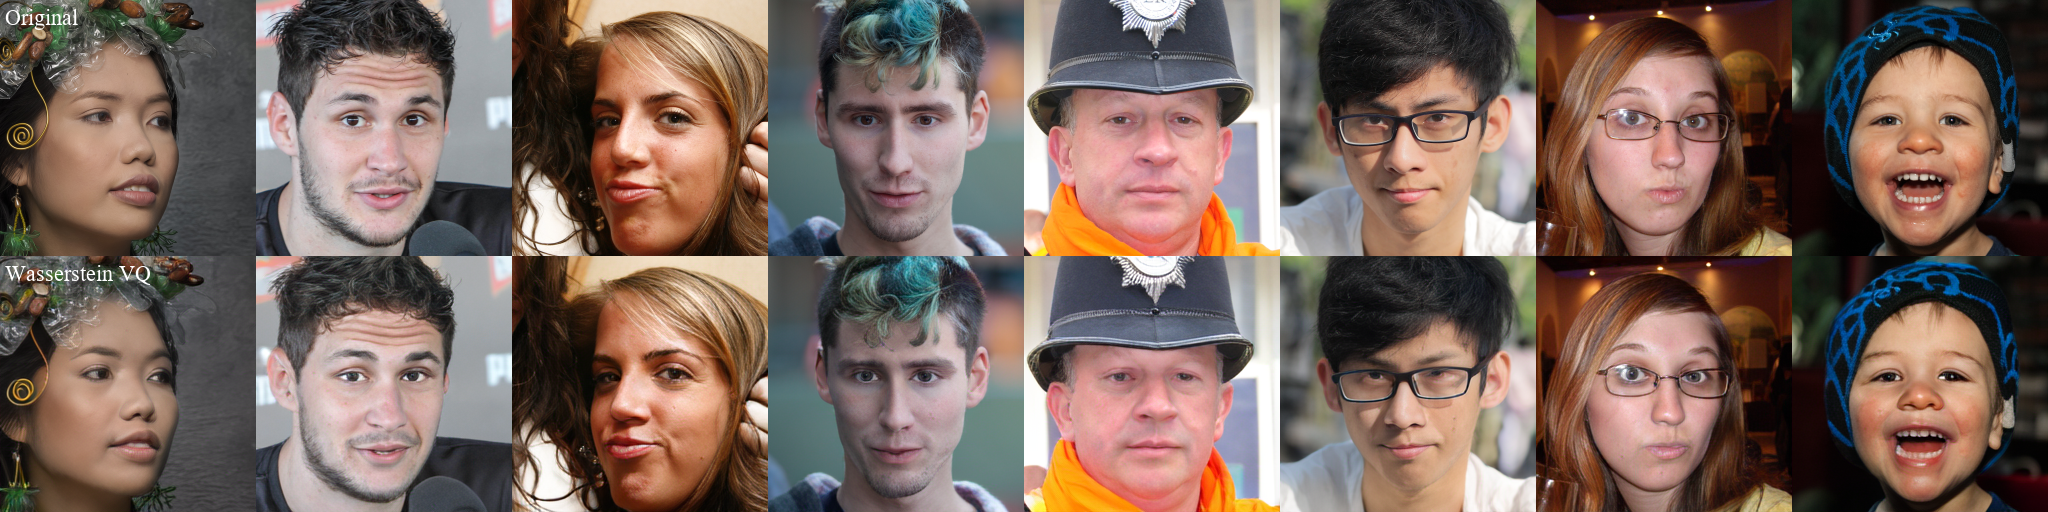
\includegraphics[width=0.92\linewidth]{figs/reconstruction/VQ_Visualization_On_FFHQ.png}
    \vspace{-1ex}
    \caption{Visualization of reconstructed FFHQ Images. The top row displays the original input images with a resolution of $256 \times 256$ pixels, while the bottom row shows the reconstructed images from the \emph{Wasserstein VQ}.}
    \label{fig:visual reconstruction ffhq}
\end{figure*}

\noindent
\begin{figure*}[!h]
    \centering
    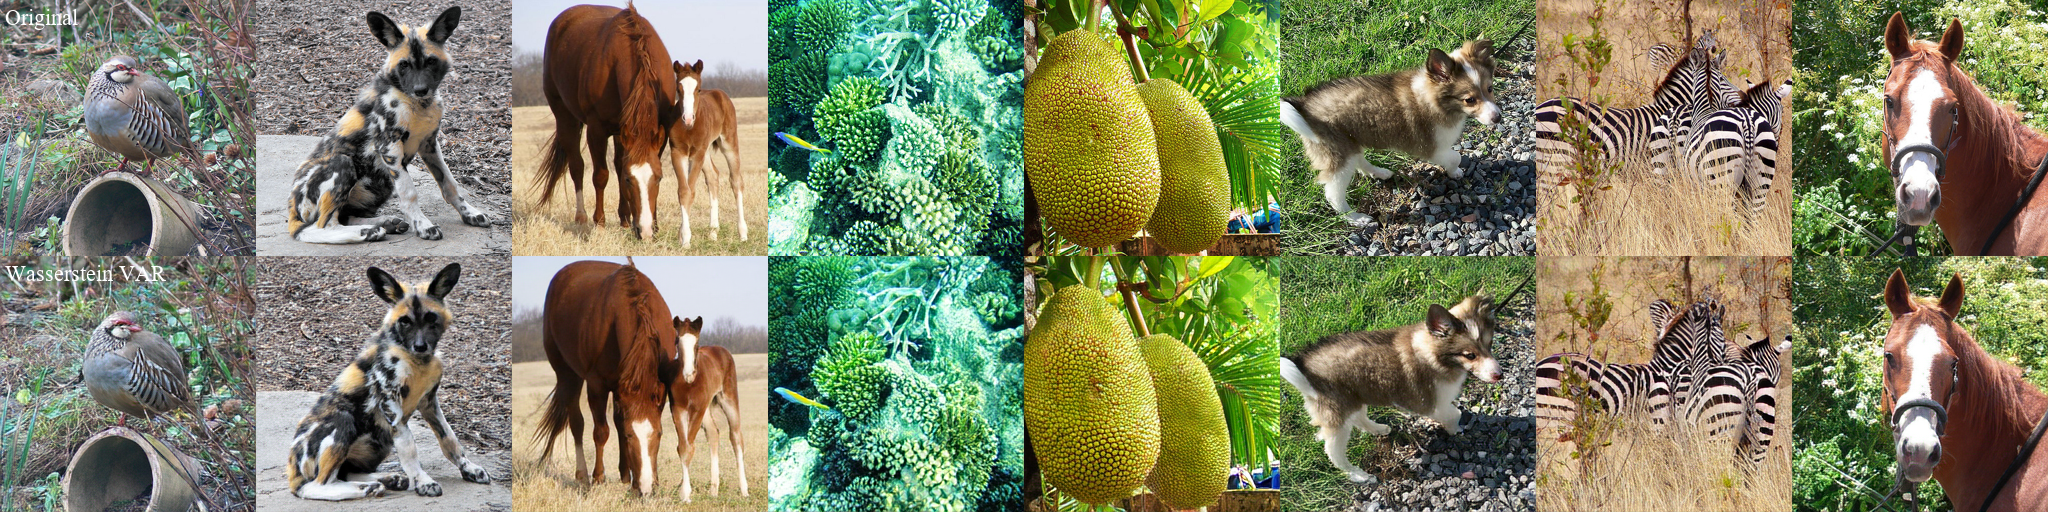
\includegraphics[width=0.92\linewidth]{figs/reconstruction/VAR_Visualization_On_ImageNet.png}
    \vspace{-1ex}
    \caption{Visualization of reconstructed ImageNet Images. The top row displays the original input images with a resolution of $256 \times 256$ pixels, while the bottom row shows the reconstructed images from the \emph{Wasserstein VAR}.}
    \label{fig:visual reconstruction imagenet}
    \vspace{-1ex}
\end{figure*}

\fi

































